%File: formatting-instructions-latex-2024.tex
%release 2024.0
\documentclass[letterpaper]{article} % DO NOT CHANGE THIS
\usepackage{aaai24}  % DO NOT CHANGE THIS
\usepackage{times}  % DO NOT CHANGE THIS
\usepackage{helvet}  % DO NOT CHANGE THIS
\usepackage{courier}  % DO NOT CHANGE THIS
\usepackage[hyphens]{url}  % DO NOT CHANGE THIS
\usepackage{graphicx} % DO NOT CHANGE THIS
\urlstyle{rm} % DO NOT CHANGE THIS
\def\UrlFont{\rm}  % DO NOT CHANGE THIS
\usepackage{natbib}  % DO NOT CHANGE THIS AND DO NOT ADD ANY OPTIONS TO IT
\usepackage{caption} % DO NOT CHANGE THIS AND DO NOT ADD ANY OPTIONS TO IT
\frenchspacing  % DO NOT CHANGE THIS
\setlength{\pdfpagewidth}{8.5in} % DO NOT CHANGE THIS
\setlength{\pdfpageheight}{11in} % DO NOT CHANGE THIS
%
% These are recommended to typeset algorithms but not required. See the subsubsection on algorithms. Remove them if you don't have algorithms in your paper.
\usepackage{algorithm}
\usepackage[noend]{algorithmic}

\usepackage{multirow}
\usepackage{subcaption}
%
% These are are recommended to typeset listings but not required. See the subsubsection on listing. Remove this block if you don't have listings in your paper.
\usepackage{newfloat}
\usepackage{listings}
\DeclareCaptionStyle{ruled}{labelfont=normalfont,labelsep=colon,strut=off} % DO NOT CHANGE THIS
\lstset{%
	basicstyle={\footnotesize\ttfamily},% footnotesize acceptable for monospace
	numbers=left,numberstyle=\footnotesize,xleftmargin=2em,% show line numbers, remove this entire line if you don't want the numbers.
	aboveskip=0pt,belowskip=0pt,%
	showstringspaces=false,tabsize=2,breaklines=true}
\floatstyle{ruled}
\newfloat{listing}{tb}{lst}{}
\floatname{listing}{Listing}
%
% Keep the \pdfinfo as shown here. There's no need
% for you to add the /Title and /Author tags.

\usepackage{amsmath}
\usepackage{amssymb}
\usepackage{amsthm}
\usepackage{mathtools}
\usepackage{bm}
\usepackage{booktabs}

\newtheorem{theorem}{Theorem}
\newtheorem{lemma}
{Lemma}
\newtheorem{assumption}{Assumption}
\newtheorem{corollary}{Corollary}
\newtheorem{remark}{Remark}


\newcommand{\la}{\langle\,}
\newcommand{\ra}{\,\rangle}
\newcommand{\argmin}{\mathop{\rm argmin}}
\newcommand{\argmax}{\mathop{\rm argmax}}

\newcommand{\lmid}{\, \middle\vert\, }

% Mathbb
\newcommand{\E}{\mathbb{E}}
\newcommand{\R}{\mathbb{R}}
\newcommand{\Z}{\mathbb{Z}}

% Mathcal
\newcommand{\cA}{\mathcal{A}}
\newcommand{\cD}{\mathcal{D}}
\newcommand{\cF}{\mathcal{F}}
\newcommand{\cS}{\mathcal{S}}
\newcommand{\cK}{\mathcal{K}}
\newcommand{\cM}{\mathcal{M}}
\newcommand{\cX}{\mathcal{X}}
\newcommand{\cP}{\mathcal{P}}
\newcommand{\cQ}{\mathcal{Q}}

\newcommand{\bphi}{\bm{\phi}}
\newcommand{\hatcP}{\widehat{\cP}}

\newcommand{\ind}[3]{{#1}^{#2}_{#3}}
\newcommand{\sind}[3]{{#1}^{#2}_{#3}}

\newcommand{\iprod}[2]{\langle #1, #2 \rangle}

\newcommand{\abs}[1]{\left|{#1}\right|}
\newcommand{\norm}[1]{\left\|{#1}\right\|_2}
\newcommand{\onlynorm}[1]{\left\|{#1}\right\|}

% RL
\newcommand{\sa}{(s,a)}
\newcommand{\optpi}{\pi^\star}

\newcommand{\algo}{\textsf{LoBiSaRL}}

% TODO
\usepackage{todonotes}
\newcommand{\aw}[1]{\todo[inline]{#1}}

% DISALLOWED PACKAGES
% \usepackage{authblk} -- This package is specifically forbidden
% \usepackage{balance} -- This package is specifically forbidden
% \usepackage{color (if used in text)
% \usepackage{CJK} -- This package is specifically forbidden
% \usepackage{float} -- This package is specifically forbidden
% \usepackage{flushend} -- This package is specifically forbidden
% \usepackage{fontenc} -- This package is specifically forbidden
% \usepackage{fullpage} -- This package is specifically forbidden
% \usepackage{geometry} -- This package is specifically forbidden
% \usepackage{grffile} -- This package is specifically forbidden
% \usepackage{hyperref} -- This package is specifically forbidden
% \usepackage{navigator} -- This package is specifically forbidden
% (or any other package that embeds links such as navigator or hyperref)
% \indentfirst} -- This package is specifically forbidden
% \layout} -- This package is specifically forbidden
% \multicol} -- This package is specifically forbidden
% \nameref} -- This package is specifically forbidden
% \usepackage{savetrees} -- This package is specifically forbidden
% \usepackage{setspace} -- This package is specifically forbidden
% \usepackage{stfloats} -- This package is specifically forbidden
% \usepackage{tabu} -- This package is specifically forbidden
% \usepackage{titlesec} -- This package is specifically forbidden
% \usepackage{tocbibind} -- This package is specifically forbidden
% \usepackage{ulem} -- This package is specifically forbidden
% \usepackage{wrapfig} -- This package is specifically forbidden
% DISALLOWED COMMANDS
% \nocopyright -- Your paper will not be published if you use this command
% \addtolength -- This command may not be used
% \balance -- This command may not be used
% \baselinestretch -- Your paper will not be published if you use this command
% \clearpage -- No page breaks of any kind may be used for the final version of your paper
% \columnsep -- This command may not be used
% % \newpage -- No page breaks of any kind may be used for the final version of your paper
% \pagebreak -- No page breaks of any kind may be used for the final version of your paperr
% \pagestyle -- This command may not be used
% \tiny -- This is not an acceptable font size.
% \vspace{- -- No negative value may be used in proximity of a caption, figure, table, section, subsection, subsubsection, or reference
% \vskip{- -- No negative value may be used to alter spacing above or below a caption, figure, table, section, subsection, subsubsection, or reference

\setcounter{secnumdepth}{2} %May be changed to 1 or 2 if section numbers are desired.

% The file aaai23.sty is the style file for AAAI Press
% proceedings, working notes, and technical reports.
%

% Title

% Your title must be in mixed case, not sentence case.
% That means all verbs (including short verbs like be, is, using,and go),
% nouns, adverbs, adjectives should be capitalized, including both words in hyphenated terms, while
% articles, conjunctions, and prepositions are lower case unless they
% directly follow a colon or long dash
\title{Long-Term Safe Reinforcement Learning with Binary Feedback}
\author {
    % Authors
    Akifumi Wachi\textsuperscript{\rm 1},
    Wataru Hashimoto\textsuperscript{\rm 2},
    Kazumune Hashimoto\textsuperscript{\rm 2}
}
\affiliations {
    % Affiliations
    \textsuperscript{\rm 1} LINE Corporation \\
    \textsuperscript{\rm 2} Osaka University \\
    akifumi.wachi@linecorp.com, hashimoto@is.eei.eng.osaka-u.ac.jp, hashimoto@eei.eng.osaka-u.ac.jp
}

%Example, Single Author, ->> remove \iffalse,\fi and place them surrounding AAAI title to use it
\iffalse
\title{My Publication Title --- Single Author}
\author {
    Author Name
}
\affiliations{
    Affiliation\\
    Affiliation Line 2\\
    name@example.com
}
\fi

\iffalse
%Example, Multiple Authors, ->> remove \iffalse,\fi and place them surrounding AAAI title to use it
\title{My Publication Title --- Multiple Authors}
\author {
    % Authors
    First Author Name,\textsuperscript{\rm 1}
    Second Author Name, \textsuperscript{\rm 2}
    Third Author Name \textsuperscript{\rm 1}
}
\affiliations {
    % Affiliations
    \textsuperscript{\rm 1} Affiliation 1\\
    \textsuperscript{\rm 2} Affiliation 2\\
    firstAuthor@affiliation1.com, secondAuthor@affilation2.com, thirdAuthor@affiliation1.com
}
\fi


% REMOVE THIS: bibentry
% This is only needed to show inline citations in the guidelines document. You should not need it and can safely delete it.
\usepackage{bibentry}
% END REMOVE bibentry

\begin{document}

\maketitle

\begin{abstract}
Safety is an indispensable requirement for applying reinforcement learning (RL) to real problems.
Although there has been a surge of safe RL algorithms proposed in recent years, most existing work typically 1) relies on receiving numeric safety feedback; 2) does not guarantee safety during the learning process; 3) limits the problem to a priori known, deterministic transition dynamics; and/or 4) assume the existence of a known safe policy for any states.
Addressing the issues mentioned above, we thus propose Long-term Binary-feedback Safe RL (\algo), a safe RL algorithm for constrained Markov decision processes (CMDPs) with binary safety feedback and an unknown, stochastic state transition function.
\algo~optimizes a policy to maximize rewards while guaranteeing a long-term safety that an agent executes only safe state-action pairs throughout each episode with high probability.
Specifically, \algo~models the binary safety function via a generalized linear model (GLM) and conservatively takes only a safe action at every time step while inferring its effect on future safety under proper assumptions.
Our theoretical results show that \algo~guarantees the long-term safety constraint, with high probability.
Finally, our empirical results demonstrate that our algorithm is safer than existing methods without significantly compromising performance in terms of reward.
\end{abstract}

\section{Introduction}
\label{sec:introduction}

Safe reinforcement learning (RL) is a promising paradigm for applying RL algorithms to real-world applications \cite{garcia2015comprehensive}.
Safe RL is beneficial in safety-critical decision-making problems, such as autonomous driving, healthcare, and robotics, where safety requirements must be incorporated to prevent RL policies from posing risks to humans or objects \cite{dulac2021challenges}.
As a result, safe RL has received significant attention in recent years as a crucial issue of RL during both the learning and execution phases \cite{amodei2016concrete}.

Safe RL is typically formulated as \textit{constrained} policy optimization problems where the expected cumulative reward is maximized while guaranteeing or encouraging the satisfaction of safety constraints, which are modeled as constrained Markov decision processes (CMDPs, \citet{altman1999constrained}).
While there are various types of constraint representations, most of the existing studies formulated constraints using either expected cumulative safety-cost~\cite{altman1999constrained} or conditional value at risk (CVaR, \citet{rockafellar2000optimization}); thus, satisfying safety constraints almost surely or with high probability received less attention to date.
Imagine highly safety-critical applications (e.g., autonomous driving, healthcare, robotics) where even a single constraint violation may result in catastrophic failure.
In such cases, RL agents need to ensure safety at every time step at least with high probability; thus, constraint satisfaction “on average” does not fit the purpose due to a large number of unsafe actions during the learning process~\cite{stooke2020responsive}.

\begin{figure}[t]
    \centering
    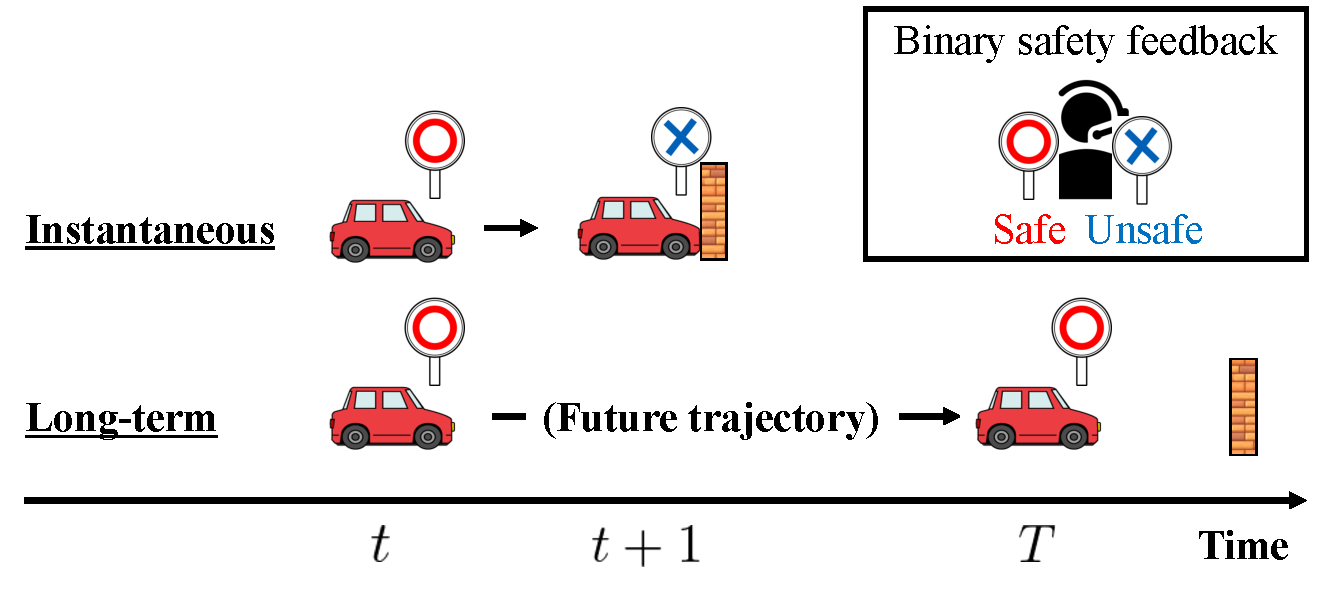
\includegraphics[width=80mm]{figures/concept.pdf}
    \caption{Even if safety is guaranteed at time $t$ based on the instantaneous evaluation, safe behavior may not exist a few steps ahead. This paper requires an agent to guarantee long-term safety (i.e., constraint satisfaction from the time the current time step $t$ to the terminal time step $T$) in CMDPs with stochastic state transition and binary safety feedback.}
    \label{fig:concept}
\end{figure}

\begin{table*}[t]
\centering
\begin{small}
\begin{tabular}{lccccc}
\toprule
& \multicolumn{2}{c}{State transition} & \multirow{2}{*}[-2pt]{Safety} & \multirow{2}{*}[-2pt]{Additional assumption(s)} \\
\cmidrule(lr){2-3}
& Known & D/S & & \\
\midrule
\citet{wachi2020safe} & Yes & D & GP & - \\
\citet{amani2021safe} & Linear & S & Linear & Known safe policy \\
\citet{wachi2021safe} & Yes & D & GLM & - \\
\citet{bennett2023provable} & No & S & GLM & Known safe policy \\
\algo~(Ours) & No & S & GLM & Lipschitz continuity \& conservative policy \\
\bottomrule
\end{tabular}
\end{small}
\caption{Comparison among existing work regarding their assumptions on a state transition, safety function, and others. In the above table, D means deterministic state transition, and S means stochastic state transition.}
\label{tab:problem}
\end{table*}

Several previous work on safe RL aimed to guarantee safety at every time step with high probability, even during the learning process.
Unfortunately, however, existing work has room for improvement.
First, most of the previous work \cite{wachi2020safe, amani2021safe, roderick2021provably, wachi2023safe} assumes numeric safety feedback.
In many cases, however, the safety feedback can only take binary values indicating whether a state-action pair is safe or unsafe, which is particularly true when feedback comes from humans.
As existing studies on safe RL with binary safety feedback, \citet{wachi2021safe} modeled the safety function via a generalized linear model (GLM) while they assume known and deterministic state transition function.
Thus, this previous work cannot deal with general RL problems with unknown stochastic state transition functions.
Also, \citet{bennett2023provable} addressed safe RL problems with binary safety feedback and unknown stochastic state transition under the assumption that a known safe action always exists for any state.
This assumption is not valid in many safety-critical applications.
For example, even an F1 driver cannot take a safe action if a vehicle traveling at $100$ km/h is $1$ meter ahead of a brick wall; thus, to avoid such situations, we need to consider ``long-term'' future safety under more reasonable assumptions, as shown in Figure~\ref{fig:concept}.

\paragraph{Contributions.}
%
We propose an algorithm called Long-term Binary-feedback Safe RL, \algo.
This algorithm enables us to solve safe RL problems with binary feedback and unknown, stochastic state transition while guaranteeing the satisfaction of long-term safety constraints.
\algo~guarantees safety by modeling the binary safety function via a GLM and then pessimistically estimating the future safety function values.
Our theoretical analysis shows that future safety can be pessimistically characterized by 1)~inevitable randomness due to the stochastic state transition and 2) divergence between the current policy and a reference policy to stabilize the state.
Based on this theoretical result, we optimize the policy to maximize the expected cumulative reward while guaranteeing long-term safety.
Finally, we empirically demonstrate the effectiveness of the \algo~compared with several baselines.

\section{Related Work}
\label{sec:related}

\paragraph{Safe RL.}

In typical safe RL problems, an agent must maximize the expected cumulative reward while ensuring that the expected cumulative cost is less than a threshold.
There have been a number of algorithms for solving this type of safe RL problem, as represented by constrained policy optimization \cite{achiam2017constrained}, reward constrained policy optimization \cite{tessler2018reward}, Lagrangian-based actor-critic \cite{chow2017risk}, primal-dual policy optimization~\cite{pmlr-v119-yang20h}.
In the previous papers mentioned above, however, a safety constraint is defined using the (expected) cumulative value and the constraint satisfaction is \textit{not} guaranteed during the learning process~\cite{stooke2020responsive}.
Hence, most of the existing studies deal with less strict safety constraints than our study that requires the agent to satisfy safety constraints \textit{at every time step}.
%
There has been research aimed at guaranteeing safety at every time step, even during the learning process.
For example, \citet{turchetta2016safe} proposed notable algorithms that satisfy the safety constraint with high probability by inferring the safety function via a Gaussian process (GP).
Also, \citet{wachi2021safe} proposed its extended algorithm that models the safety function via a GLM, which can also deal with safe RL problems with binary feedback.
Though they succeeded in guaranteeing safety with high probability, their theoretical results are based on the assumptions of the known and deterministic state transition function.
It is essentially difficult to extend these algorithms to our problem settings with unknown and stochastic state transitions.
As existing work on safe RL with unknown stochastic transition, \citet{amani2021safe} proposed an algorithm for linear MDPs with safety constraints while \citet{bennett2023provable} proposed an algorithm for safe RL problems with binary safety feedback and stochastic transitions.
Although such work proposed excellent algorithms for challenging problems, the existence of a known safe policy is assumed for any state, which does not hold in many real-world applications as discussed in  Section~\ref{sec:introduction} (i.e., high-speed vehicle example).
Table~\ref{tab:problem} summarizes the problem settings considered in existing work and this paper.

\paragraph{Long-term safety.}

In the control community, long-term safety has been well-studied under the name of control barrier function (CBF, \citet{ames2019control}).
For any state $s$, a CBF is a continuously differentiable function $h(s)$ that defines a safe set $\{s: h(s) \ge 0 \}$, i.e., an invariant set where any trajectory starting inside the set remains within the set.
The CBF is to maintain safety during the learning process, which is particularly useful for keeping a manipulator within a given safe space or ensuring that a robot avoids obstacles.
This advantage is beneficial for RL settings, and \citet{cheng2019end} proposed a safe RL algorithm to guarantee long-term safety via CBFs.
Unfortunately, however, humans need to manually define proper CBFs and it is often hard to find them.
In addition, \citet{koller2018learning} proposed a learning-based model predictive control scheme that provides high-probability safety guarantees during the learning process under the assumption that both a dominant term of the state transition function and safe region are known a priori.

\section{Problem Statement}
\label{sec:problem}

We consider episodic finite-horizon CMDPs, which can be formally defined as a tuple
%
\begin{equation}
    \cM \coloneqq (\cS, \cA, P, T, r, g, s_1),
\end{equation}
%
where $\cS$ is a state space $\{s\}$,
$\cA$ is an action space $\{a\}$,
$P: \cS \times \cA \rightarrow \Delta(\cS)$ is an unknown, stochastic state transition function to map a state-action pair to a probability distribution over the next states,
$T \in \mathbb{Z}_+$ is a fixed length of each episode,
$r: \cS \times \cA \rightarrow [0, 1]$ is a (bounded) reward function,
$g: \cS \times \cA \rightarrow \{0, 1\}$ is an unknown binary safety function, and $s_1 \in \cS$ is the initial state.\footnote{We assume that reward function is known and deterministic, but all results presented here extend to unknown stochastic cases.}
Crucially, in this paper, the safety feedback is provided as a \textit{binary} value; that is, $g(s,a) = 1$ means that a state-action pair $(s,a)$ is safe, and otherwise $(s,a)$ is unsafe.
At the time step $t$ and the current state $s_t$, the agent takes the next action $a_t$, receiving the next state $s_{t+1} \sim P(\cdot \mid s_t, a_t)$ as well as the safety observation $g(s_t, a_t)$, until the terminal time step $T$.
%
We suppose that safety observations contain some independent zero-mean noise $n_t$.
We assume that the noise $n_t$ is sub-Gaussian with fixed (positive) parameters $\sigma \in \R_+$; that is, for all $t$, we have $\mathbb{E} \left [\, e^{\omega n_t} \mid \mathcal{G}_{t-1}\,\right] \le e^{\omega^2 \sigma^2/2}$,
%
where $\{\mathcal{G}_{t}\}$ is increasing sequences of sigma fields such that $n_t$ is $\mathcal{G}_{t}$-measurable with $\mathbb{E} \left[\, n_t \mid \mathcal{G}_{t-1}\, \right]=0$.
This assumption has been commonly made in previous work (e.g., \citet{NIPS2011_e1d5be1c}, \citet{li2017provably}).

A deterministic policy of an agent $\pi: \cS \rightarrow \cA$ represents a function to return actions.
A metric of the quality of the policy $\pi$ is the following value function, i.e., the expected value of cumulative rewards, which is defined as
%
\begin{equation*}
 \sind{V}{\pi}{t}(s) \coloneqq \E_{\pi} \left[\, \sum_{\tau=t}^T r(s_\tau, a_\tau)  \, \bigg | \, s_t = s \,\right],
\end{equation*}
%
for all $s \in \cS$ and $t \in [T]$,
where the expectation $\E_\pi[\cdot]$ is taken over the trajectories $\{(s_\tau, a_\tau)\}_{\tau=t}^T$ induced by the policy $\pi$ and true state transition dynamics $P$.
%
We additionally define the following action-value function (i.e., Q-function) which means the expected value of total rewards when the agent starts
from state-action pair $(s,a)$ at step $t$ and follows policy $\pi$, which is represented as
%
\begin{equation*}
    \sind{Q}{\pi}{t}(s,a) \coloneqq \E_{\pi} \left[\, \sum_{\tau=t}^T r(s_\tau, a_\tau) \, \bigg |\, s_t = s, a_t = a \,\right],
\end{equation*}
%
for all $(s,a) \in \cS\times \cA$ and $t \in [T]$.

A crucial point of this paper is that we wish the agent to take only \textit{safe} actions at every time step $t$; that is, the agent needs to take a safe action $a_t$ at a state $s_t$ that satisfies the safety constraint; that is, $g(s_t, a_t) = 1$.
As discussed in Section~\ref{sec:introduction}, however, at time $t$, the agent is required to execute safe actions in the long run so that there also will be future safe actions from time $t+1$ to $T$.
Hence, at every time step $t$, we impose the following safety requirement:
%
\begin{equation}
    \label{eq:constraint}
    \Pr \Bigl\{ g(s_\tau, a_\tau) = 1 \quad \forall \tau \in [t, T] \Big\} \ge 1 - \delta,
\end{equation}
%
where $\delta \in [0, 1]$ is a small positive scalar.
Our safety constraint is probabilistic since it is extremely difficult to guarantee safety almost surely (i.e., probability of $1$) due to the unknown stochastic state transition and safety functions.

\paragraph{Goal.}
Let us clearly describe the goal we wish to achieve in this paper.
%
The objective of the agent is to obtain the optimal policy $\pi^\star: \cS \rightarrow \cA$ to maximize the value function $V^\pi_t(s_t)$ under the safety constraint \eqref{eq:constraint} such that
%
\begin{align*}
    \label{eq:opt}
    \max_{\pi} V^\pi_t(s_t)
    \ \  \text{s.t.} \ \
    \Pr \Bigl\{ g(s_\tau, a_\tau) = 1 \ \ \forall \tau \in [t, T] \Big\} \ge 1 - \delta.
\end{align*}
%
It is quite hard to guarantee the satisfaction of the aforementioned constraint.
It is because even if the agent executes an action $a_t$ at time $t$ and state $s_t$ such that
%
\begin{equation}
    \label{eq:short_constraint}
    \Pr\Bigl\{ g(s_t, a_t) = 1 \Big\} \ge 1 - \delta,
\end{equation}
%
there may \textit{not} be any viable action at $s_{t+1} \sim P(s_t, a_t)$ and further future states.
Thus, the agent must execute an action $a_t$ to guarantee the constraint satisfaction not only for $(s_t, a_t)$ but also for $(s_\tau, a_\tau)$ for all $\tau \in [t+1, T]$.
Our safety constraint \eqref{eq:constraint} is challenging, which we will call the \textit{long-term} safety constraint in the rest of this paper, while we will call~\eqref{eq:short_constraint} the \textit{instantaneous} safety constraint.

\paragraph{Difficulties and assumptions.}

The aforementioned problem we wish to solve has several difficulties.
First, if the binary safety function does not exhibit any regularity, it is impossible to infer the safety of state-action pairs.
For example, if the safety function value is totally random, we can neither foresee danger nor guarantee safety.
In addition, we suppose the state transition is stochastic and unknown a priori despite that the agent must guarantee the satisfaction of the long-term safety constraint.
This difficulty requires us to explicitly incorporate the stochasticity of the state transition and its influence on future safety.

For the first difficulty, we assume that the safety function can be modeled as a GLM to deal with binary safety feedback.
GLMs have been studied for sequential decision-making problems with binary feedback especially in (stateless) multi-armed bandit literature~\citep{filippi2010parametric,li2017provably,faury2020improved} under the name of logistic bandits.
Also, in (stateful) RL settings, \citet{wachi2021safe} addressed a safe RL problem where the safety function is subject to a GLM under the assumption that the state transition is a priori known and deterministic.
We now make the following assumption of the GLM structure of the safety function.
%
\begin{assumption}
\label{assumption:linear}
There exists a known feature mapping function $\bphi: \cS \times \cA \rightarrow \R^m$, unknown coefficient vectors $\bm{w}^\star \in \R^m$, and a fixed, strictly increasing (inverse) link function $\mu: \R \rightarrow [0, 1]$ such that
%
\begin{align}
\label{eq:gl_safety}
    \E[\, g(s, a) \mid s, a \,] = \mu\bigl(f^\star(s,a)\bigr),
\end{align}
%
for all $(s, a) \in \cS \times \cA$,
where $f^\star: \cS \times \cA \rightarrow \R$ is a linear predictor defined as
%
\begin{align}
    f^\star(s, a) \coloneqq \iprod{\bphi(s,a)}{\bm{w}^\star}, \quad \forall (s, a) \in \cS \times \cA.
\end{align}
%
Without loss of generality, we further assume $\norm{\bphi(s, a)} \le 1$ for all $(s,a) \in \cS \times \cA$ and $\norm{\bm{w}^\star} \le \sqrt{m}$.
\end{assumption}
%
\noindent
In the case of the binary safety function, a suitable choice of the link function is $\mu(x) = \exp(x)/(1 + \exp(x))$, leading to the logistic regression model.
GLMs are more general models, and one can verify that linear and integer-valued functions are special cases of GLMs with $\mu(x) = x$ and $\mu(x) = \exp(x)$ leading to the linear regression model and the Poisson regression model, respectively; hence, our method can be extended to other problem settings than the binary safety function.

In addition to the boundedness assumption on the feature vectors and safety function values, we make the following assumption regarding the link function.
%
\begin{assumption}
\label{assumption:link}
The link function $\mu$ is twice differentiable, and the first and second-order derivatives are respectively bounded.
Also, the link function $\mu$ satisfies $\xi = \inf_{\| \bm{w} - \bm{w}^\star \| \le 1, \|\bm{\phi}\| \le 1} \dot{\mu}(\iprod{\bm{\phi}} {\bm{w}}) > 0$.
\end{assumption}

By making Assumptions~\ref{assumption:linear} and \ref{assumption:link}, it is possible to guarantee the satisfaction of the instantaneous safety constraint~\eqref{eq:short_constraint} at the current time step $t$ if there are feasible actions, as conducted in \citet{wachi2021safe}.
In this paper, however, the agent must guarantee safety until the terminal time step $T$ (i.e., long-term safety constraint) under stochastic state transition, which requires us to make further assumptions.
If the feature mapping function drastically changes with minor differences in state-action pairs, it is extremely difficult to continue to guarantee safety until $T$.
Thus, we assume the regularity of the feature mapping function as a form of Lipschitz continuity, which is written as follows:
%
\begin{assumption}
\label{assumption:lipschitz_feature}
For all $s, \bar{s} \in \cS$ and $a, \bar{a} \in \cA$, the feature mapping function $\bphi(\cdot, \cdot)$ is Lipschitz continuous with a constant $L_\phi \in \R_{+}$; that is,
%
\begin{equation}
    \norm{\bphi(s, a) - \bphi(\bar{s}, \bar{a})} \le L_\phi \cdot d_{\cS\cA}((s, a), (\bar{s}, \bar{a})),
\end{equation}
%
where $d_{\cS\cA}(\cdot, \cdot)$ is a distance metric on $\cS \times\cA$.
For ease of exposition, we assume that $d_{\cS\cA}$ satisfies $d_{\cS\cA}((s, a), (\bar{s}, \bar{a})) = d_\cS(s, \bar{s}) + d_\cA(a, \bar{a})$.
\end{assumption}
%
\noindent
Intuitively, this assumption implies that, for similar state-action pairs $(s,a)$ and $(\bar{s}, \bar{a})$, the features $\bphi(s, a)$ and $\bphi(\bar{s}, \bar{a})$ also exhibit similar values.
This assumption is related to the common assumption in RL literature as represented by Lipschitz MDP~\cite{asadi2018lipschitz,ok2018exploration}.

Similarly, at a current state $s$, if the next state $s' \sim P(\cdot \mid s, a)$ induced by an ``insignificant'' action $a$ (that tries to maintain the status quo) is far from $s$, the safety may drastically changes.
Hence, we assume the existence of a Lipschitz-continuous conservative policy $\pi^\sharp: \cS \rightarrow \cA$ to suppress the state transition distance within a certain value.
We then assume that, as far as similar policies to the conservative policy are executed, the state-transition distance can be suppressed.
Specifically, for any policy $\pi$, we assume that the (one-step) state transition from time $t$ to $t+1$ is upper-bounded according to the divergence between the actions taken by $\pi$ and $\pi^\sharp$.
%
\begin{assumption}
    \label{assumption:stabilizing}
    Let $L_\sharp \in \R_+$ be a positive scalar.
    There exists a known $L_\sharp$-Lipschitz continuous policy $\pi^\sharp: \cS \rightarrow \cA$ such that, for any states $s, \bar{s} \in \cS$,
    %
    \begin{equation}
        d_\cA(\pi^\sharp(s) - \pi^\sharp(\bar{s})) \le L_\sharp \cdot d_\cS(s, \bar{s}).
    \end{equation}
    %
    Also, with a positive scalar $\eta \in \R_{+}$, for any policy $\pi: \cS \rightarrow \cA$, the following inequality holds for all $s \in \cS$:
    %
    \begin{equation*}
        \max_{s' \sim P(\cdot \mid s, \pi(s))} d_\cS(s, s') \le \bar{d} + \eta \cdot d_\cA(\pi(s), \pi^\sharp(s)).
    \end{equation*}
\end{assumption}

\begin{remark}
    Assumption~\ref{assumption:stabilizing} implies that the conservative policy $\pi^\sharp$ keeps the amount of the (one-step) state transition within a certain distance $\bar{d} \in \R_{+}$; that is,
    %
    \begin{equation*}
        \max_{s' \sim P(\cdot \mid s, \pi^\sharp(s))} d_\cS(s, s') \le \bar{d}.
    \end{equation*}
\end{remark}

\noindent
In the case of stochastic policies, we can use Kantorovich distance $K(\cdot, \cdot)$ to define the Lipschitz continuity of a policy; that is, $K(\pi(\cdot \mid s), \pi(\cdot \mid \bar{s})) \le L_\pi \cdot d_\cS(s, \bar{s})$.
Thus, the following theoretical analysis can be extended to stochastic policy settings.
This assumption is valid in many physical systems (e.g., control-affine systems).
Intuitively, when the policy $\pi$ is similar to the conservative policy $\pi^\sharp$, the upper bound of the state transition is guaranteed to be small.
Assumption~\ref{assumption:stabilizing} implies that when $\pi = \pi^\sharp$, the state transition distance is always less than or equal to $\bar{d}$.
Also, as $\pi$ becomes far from $\pi^\sharp$, the distance can be larger with respect to the term $\eta \cdot d_\cA (\pi, \pi^\sharp$).
The existence of $\pi^\sharp$ is not restrictive in practice for a number of applications, and similar notions have been adopted in many existing studies under the name of the stable or telescoping policies \cite{lin2021perturbation,tsukamoto2021contraction}.
For instance, with the autonomous vehicle, one may select
$\pi^\sharp$ as the one to move it at a low constant speed,
and $\pi$ is optimized such that it can move faster under the safety constraint.


\section{Characterizing Safety}
\label{sec:preliminary}

Based on the problem settings and assumptions presented in Section~\ref{sec:problem}, we now present how to guarantee long-term safety.
Optimism and pessimism are essential notions in RL.
Conventionally, being optimistic has been well-adopted in online RL literature under the name of optimism in the face of uncertainty principle~\cite{strehl2008analysis,auer2007logarithmic}.
In contrast, pessimism is also significant when an RL agent is trained from offline data~\cite{jin2021pessimism,buckman2020importance} or needs to satisfy safety constraints~\cite{bura2022dope}.
%
A natural way to incorporate optimism and pessimism is to derive the upper and lower bounds of the functions of interest, which can be conducted in a way backed by theory.

This paper expresses the upper and lower bounds in two ways.
The first is inferred by the GLMs.
While the advantage of this approach is to provide accurate estimation once a larger amount of dataset has been collected, the uncertainty term tends to be loose in the early phase of the training.
The second is based on Lipschitz continuity.
In contrast to the GLM-based approach, this approach provides moderate bounds regardless of the amount of collected data, which is typically useful in the early phase of training.
Thus, intuitively, we aim to continue to derive tight bounds by deriving them using the approach based on Lipschitz continuity in the early phase and that based on the GLMs in the later phase.


\subsection{Confidence Intervals Inferred by GLMs}
\label{sec:bound_glm}

We first present how to obtain theoretically-guaranteed confidence bounds inferred by the GLMs.
Hereinafter, let the design matrix be
%
$W_n = \sum_{j=1}^n \bm{\phi}(s_j, a_j) \bm{\phi}(s_j, a_j)^\top$, where $n \in \mathbb{Z}_+$ is the total number of data.
%
Also, the weighted $L_2$-norm of $\bm{\phi}$ associated with $W_n^{-1}$ is given by
$\onlynorm{\bm{\phi}}_{W_n^{-1}} \coloneqq \sqrt{\bm{\phi}^\top W_n^{-1} \bm{\phi}}$.
%
Here, the maximum-likelihood estimators (MLE) denoted as $\hat{\bm{w}}$ is calculated by solving the following equation:
%
\begin{equation*}
    \sum_{j=1}^n \bigl(g(s_j, a_j) - \mu(\la \bphi(s_j, a_j), \bm{w} \ra) \bigr) \bphi(s_j, a_j) = 0,
\end{equation*}
%
Based on \citet{li2017provably}, the following lemma regarding the confidence bounds on $f^\star$ holds.
%
\begin{lemma}
\label{lemma:confidence_bound}
Let $\Delta > 0$ be given and $\beta = \frac{3 \sigma}{\xi} \sqrt{\log \frac{3}{\Delta}}$.
%
Then, with a probability of at least $1-\Delta$, the MLE satisfies
%
\begin{alignat*}{2}
\abs{f^\star(s,a) - \iprod{\bphi(s,a)}{\hat{\bm{w}}}} \le \beta \cdot \onlynorm{\bphi(s,a)}_{W_n^{-1}},
\end{alignat*}
%
for all $(s,a) \in \cS \times \cA$.
\end{lemma}
%
\noindent
Therefore, at time $t$ and state $s_t$, by choosing the next action $a_t$ such that $\iprod{\bphi(s_t, a_t)}{\hat{\bm{w}}} - \beta \cdot \onlynorm{\bphi(s_t, a_t)}_{W_n^{-1}} \ge z$, we can also guarantee the satisfaction of $f^\star(s_t, a_t) \ge z$ with high probability, where $z \in \R$ is a certain threshold.

\subsection{Bounds by Lipschitz Continuity}
\label{sec:bound_lipschiz}

We then present the upper and lower bounds inferred by the Lipschitz continuity.
Let us first define an important variable $x_t \in \R_+$ called maximum divergence from the conservative policy (MDCP) such that
%
\begin{equation}
    \label{eq:policy_x_t}
    d_\cA(\pi(s_t), \pi^\sharp(s_t)) \le x_t, \quad \forall t \in [T].
\end{equation}
%
The MDCP indicates how far the action taken by $\pi$ is from that by $\pi^\sharp$.
Hereinafter, the summation of this new variable $x_t$ plays a critical role when dealing with the long-term safety constraint, and thus we define $X_{t_1}^{t_2} \coloneqq \sum_{\tau=t_1}^{t_2} x_\tau$ for any time steps $t_1, t_2 \in [T]$ with $t_1 < t_2$.
%
We have the following two lemmas regarding the (true) safety linear predictor $f^\star$.
See Appendices \ref{proof:A_2} and \ref{proof:A_3} for the proofs.
% See Appendices A.2 and A.3 for the proofs.

\begin{lemma}
    \label{lemma:f_t_T}
    Suppose the policy $\pi$ satisfies \eqref{eq:policy_x_t}.
    Let $L_1$, $L_2$, and $L_3$ be constants that are respectively defined as
    \[
        L_1 \coloneqq \sqrt{m} \cdot L_\phi, L_2 \coloneqq \bar{L}_\sharp \cdot \bar{d}, L_3 \coloneqq 2 + \eta \bar{L}_\sharp.
    \]
    %
    Set $\bar{t} \coloneqq T - t$ and
    recall that $X_{t+1}^{T-1} \coloneqq \sum_{\tau=t+1}^{T-1} x_\tau$.
    Finally, with $x_{t:T} \coloneqq x_t, x_{t+1}, \ldots, x_T$, define
    %
    \begin{equation*}
        \mathcal{F}(t, x_{t:T}) \coloneqq L_1 \left\{L_2 \bar{t} + (L_3-1) x_t + L_3 X_{t+1}^{T-1} + x_{T} \right\}.
    \end{equation*}
    %
    Then, we have
    %
    \begin{align*}
        \abs{f^\star(s_T, \pi(s_T)) - f^\star(s_t, \pi(s_t))}
        \le \mathcal{F}(t, x_{t:T}).
    \end{align*}
\end{lemma}
%
\noindent
Intuitively, Lemma~\ref{lemma:f_t_T} characterizes the present-to-future difference in terms of $f^\star$, which provides us the lower bound of the future safety linear predictor.
%
\begin{lemma}
    \label{lemma:f_1_t}
    Define $f^\sharp(s) \coloneqq f^\star(s, \pi^\sharp(s))$ for all $s \in \cS$.
    Also, suppose the policy $\pi$ satisfies \eqref{eq:policy_x_t}.
    Then, we have
    \begin{align*}
        \abs{f^\star(s_t, \pi(s_t)) - f^\sharp(s_1)}
        \le L_1 \left\{L_2 \, t + L_3 X_{2}^{t-1} + x_{t} \right\}.
    \end{align*}
\end{lemma}
%
\noindent
In contrast to Lemma~\ref{lemma:f_t_T}, Lemma~\ref{lemma:f_1_t} characterizes the past-to-present difference in terms of $f^\star$.
Using this lemma, we infer the lower bound of $f^\star$ at the current time step $t$.

\begin{figure*}[t]
    \centering
    \begin{subfigure}[b]{0.33\textwidth}
        \centering
        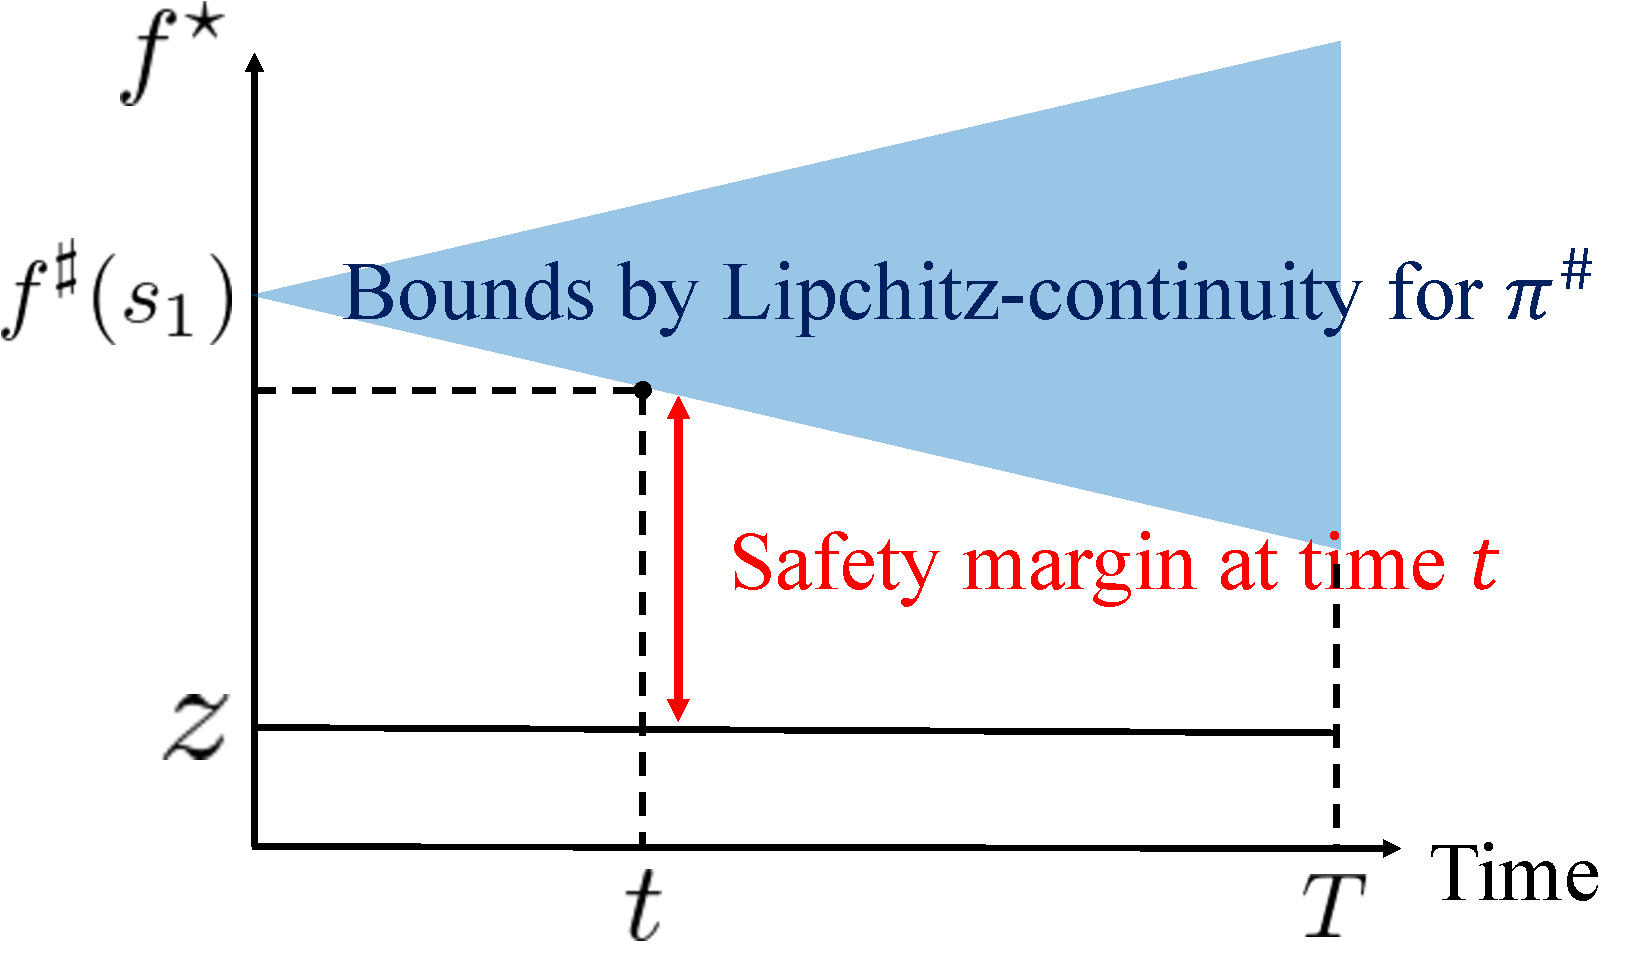
\includegraphics[width=\textwidth]{figures/fig_1.pdf}
        \caption{Conservative policy}
        \label{fig:point_return}
    \end{subfigure}
    \hfill
    \begin{subfigure}[b]{0.33\textwidth}
        \centering
        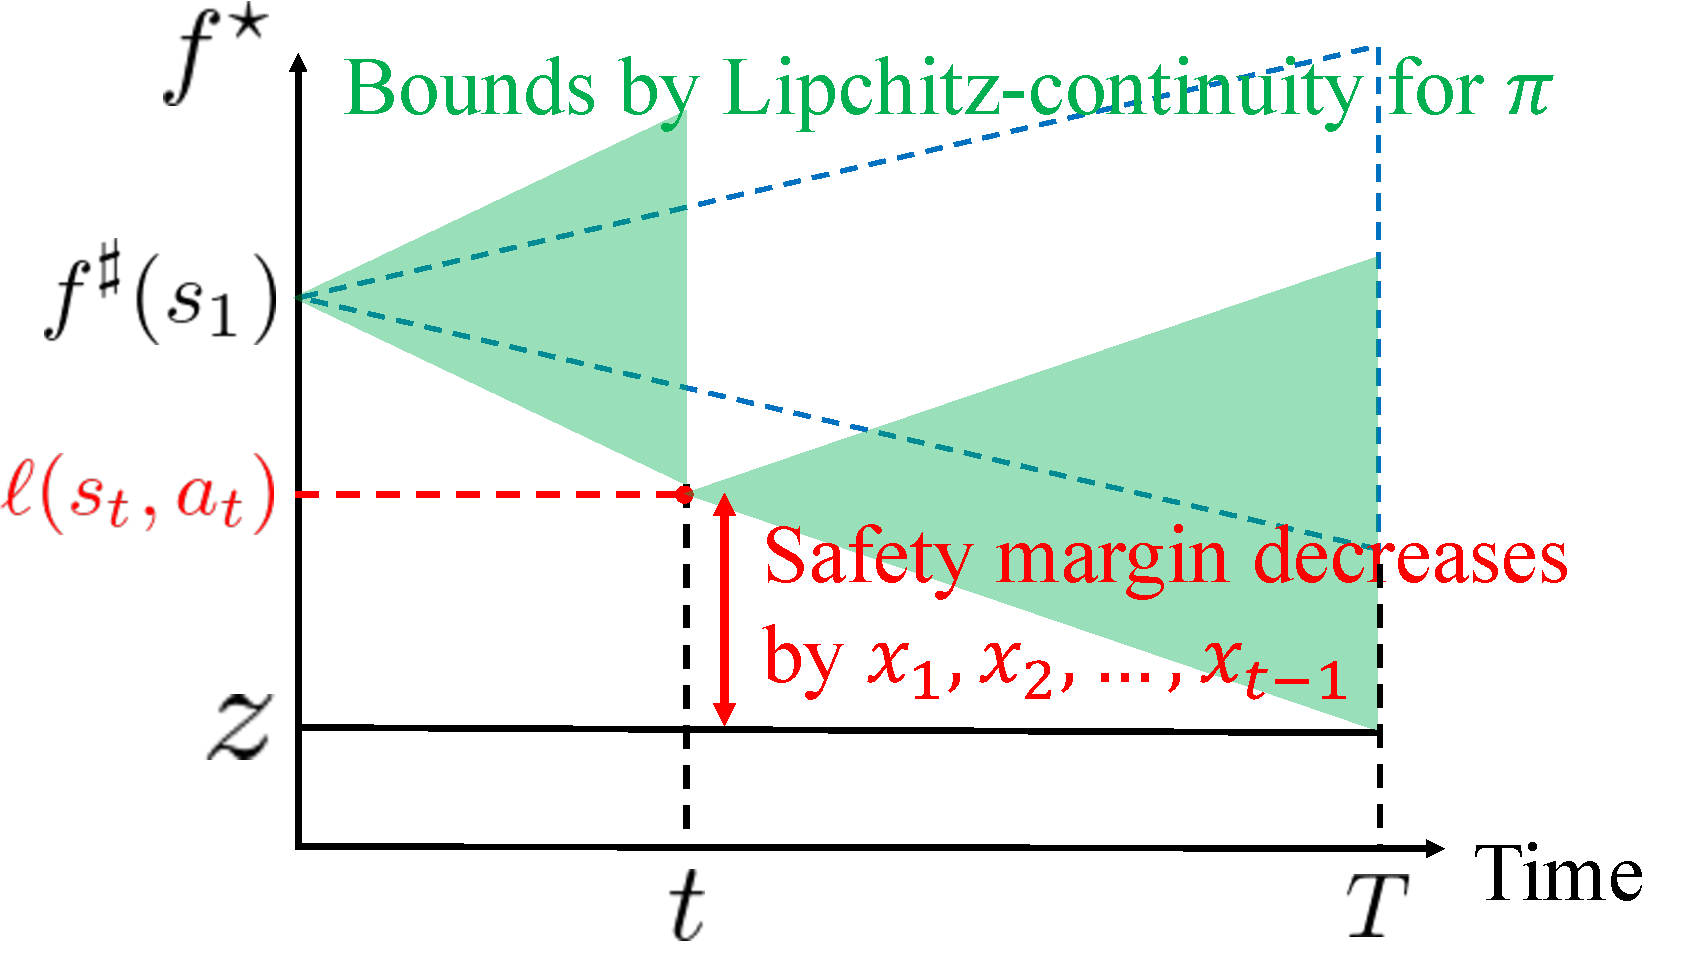
\includegraphics[width=\textwidth]{figures/fig_2.pdf}
        \caption{Early phase (Lipschitz)}
        \label{fig:point_avecost}
    \end{subfigure}
    \hfill
    \begin{subfigure}[b]{0.33\textwidth}
        \centering
        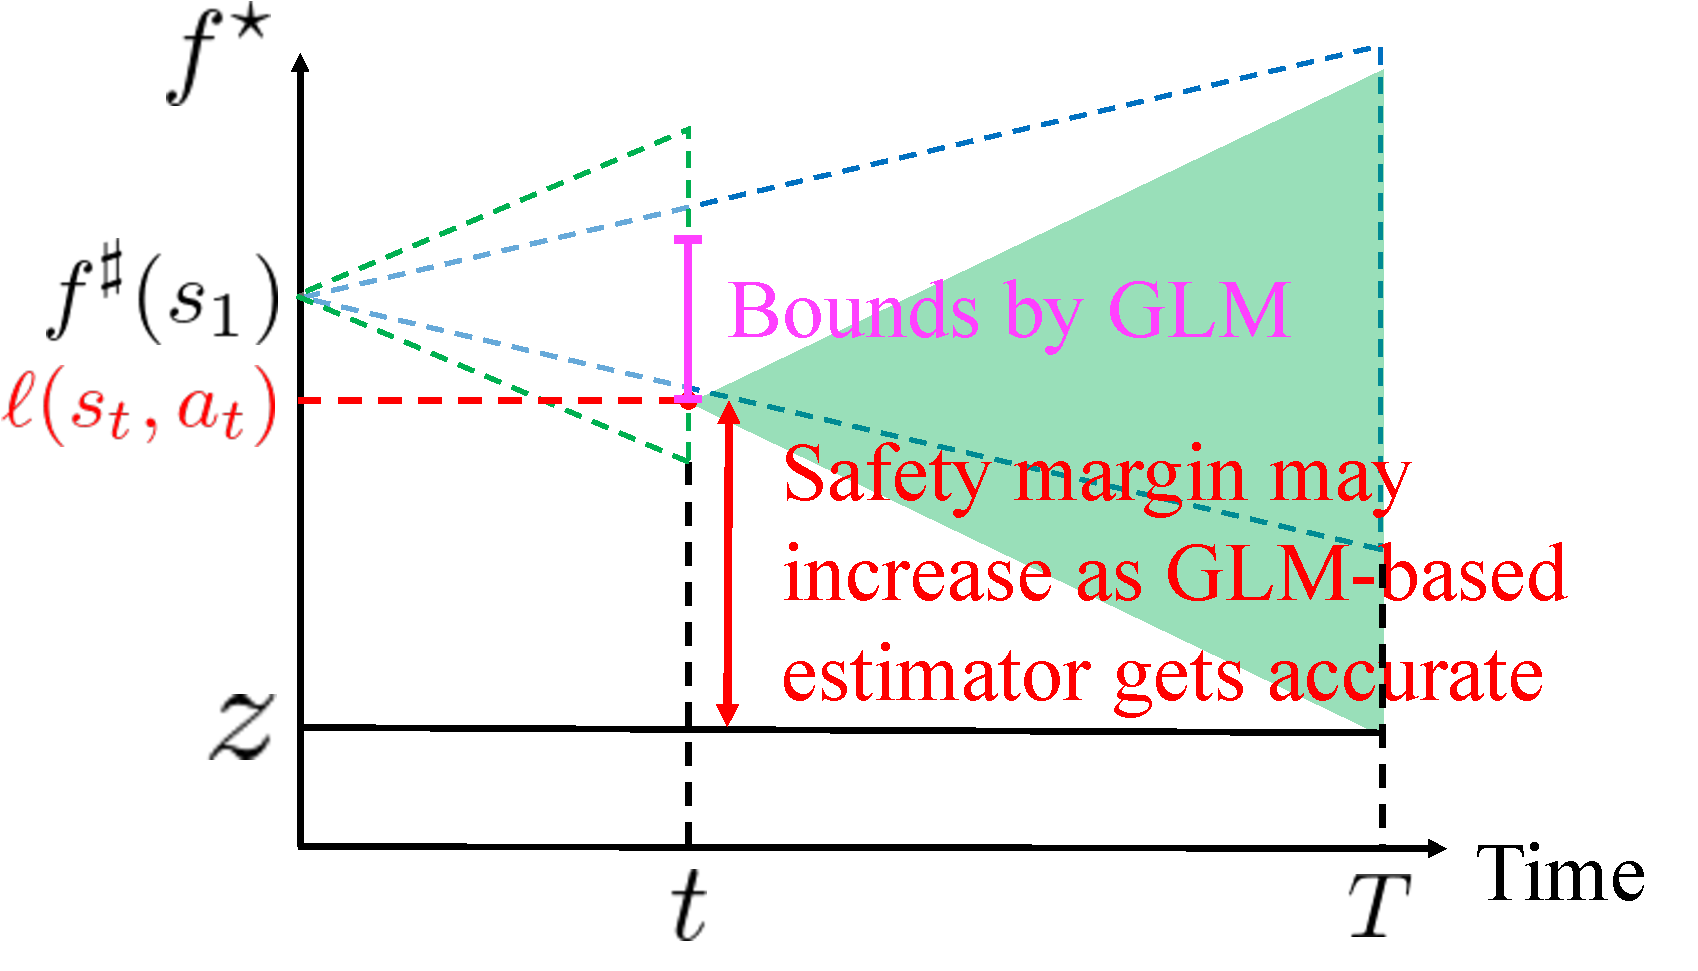
\includegraphics[width=\textwidth]{figures/fig_3.pdf}
        \caption{Later phase (GLM)}
        \label{fig:point_maxcost}
    \end{subfigure}
    \caption{(a) Bounds by Lipschitz continuity for the conservative policy. (b) In the early phase of training, the lower bound of the safety linear predictor at time $t$ is typically characterized by the Lipschitz continuity, which decreases depending on the $x_1, x_2, \ldots, x_{t-1}$. Depending on the safety margin at time $t$, we need to control $x_{t}, x_{t+1}, \ldots, x_T$ for ensuring future safety. (c) As the training proceeds, the lower bound of the safety linear predictor can potentially be characterized by the GLMs, and the safety margin may increase.}
    \label{fig:long_term_safety}
\end{figure*}

\subsection{Resulting Lower Bound of $\bm{f^\star}$}

As we discussed previously, it is a simple yet powerful way to use the safety lower bound for introducing pessimism in safe RL.
Let $\ell: \cS \times \cA \rightarrow \R$ denote a lower bound of the true safety linear predictor, $f^\star$.
%
To obtain a tighter bound, this paper combines the two lower bounds presented in Section~\ref{sec:bound_glm} and \ref{sec:bound_lipschiz}, respectively.
Specifically, based on Lemma~\ref{lemma:confidence_bound} and \ref{lemma:f_1_t}, we obtain the following tighter bound:
%
\begin{equation}
    \ell(s_t, a_t) \coloneqq \max \bigl(\ell_\text{GLM}(s_t, a_t), \ell_\text{Lipschitz}(s_t, a_t) \bigr),
\end{equation}
%
where $\ell_\text{GLM}: \cS \times \cA \rightarrow \R$ and $\ell_\text{Lipschitz}: \cS \times \cA \rightarrow \R$ are pessimistic safety linear predictors inferred by GLM and Lipshitz continuity, which are respectively defined as
%
\begin{align*}
    \ell_\text{GLM}(s_t, a_t)
    \coloneqq &\ \iprod{\bphi(s_t, a_t)}{\hat{\bm{w}}} - \beta \cdot \onlynorm{\bphi(s_t, a_t)}_{W_n^{-1}}, \\
    \ell_\text{Lipschitz}(s_t, a_t)
    \coloneqq &\ f^\sharp(s_1) - L_1 \left\{L_2\, t + L_3 X_{1}^{t-1} + x_{t} \right\}.
\end{align*}

\subsection{Long-term Safety Guarantee}

We present theoretical results regarding the lower bound of the safety linear predictor $f^\star$, which leads to the long-term safety guarantee defined by \eqref{eq:constraint}.
We now present a lemma regarding the safety linear predictor at time $t$.
%
\begin{lemma}
    \label{lemma:lower_bound}
    At every time step $t \in [T]$, we have
    %
    \begin{equation}
        \label{eq:f_t}
        f^\star(s_t, a_t) \ge \ell(s_t, a_t)
    \end{equation}
    %
    with a probability of at least $1-\Delta$.
\end{lemma}
%
\noindent
This lemma implies that we can guarantee the instantaneous safety constraint \eqref{eq:short_constraint} by choosing the next action such that
%
\begin{equation}
    \ell(s_t, a_t) \ge z, \quad \text{with} \quad \mu(z) = 1 - \delta,
\end{equation}
%
with a probability of at least $1 - \Delta$.

In this paper, however, we need to additionally require the satisfaction of the long-term safety constraint; thus, we are particularly interested in future safety.
We now provide the following lemma in terms of the pessimistic safety linear predictor at the terminal time step $T$:
%
\begin{lemma}
    \label{lemma:f_ell_T}
    Recall $T$ is the terminal time step and set $\bar{t} = T - t$.
    At every time step $t \in [T]$, we have
    %
    \begin{align*}
        \label{eq:f_t_T}
        f^\star(s_T, a_T)
        \ge &\ \ell(s_t, a_t) - \mathcal{F}(t, x_{t:T}),
    \end{align*}
    %
    with a probability of at least $1-\Delta$.
\end{lemma}

\begin{corollary}
    \label{corollary:safety}
    Suppose, at state $s_t$, the agent with a policy $\pi$ executes the action $a_t$ while tuning $x_t, x_{t+1}, \ldots, x_T$ so that
    %
    \begin{equation}
        \label{eq:condition_safety}
        \ell(s_t, a_t) - \mathcal{F}(t, x_{t:T}) \ge z
    \end{equation}
    holds.
    Then, for all $\tau \in [t, T]$, there exist safe state-action pairs $(s_\tau, a_\tau)$ such that:
    %
    \begin{equation}
        f^\star(s_\tau, a_\tau) \ge z, \quad \tau \in[t, T],
    \end{equation}
    %
    with a probability of at least $1 - \Delta$.
\end{corollary}
%
\noindent
The proofs of Lemma~\ref{lemma:f_ell_T} and Corollary~\ref{corollary:safety} are written in
Appendix \ref{appendix:A_5}.
% Appendix A.4.

Finally, we present a main theorem on the long-term safety constraint.
Specifically, we guarantee that an agent continues to take safe actions from time $t$ to $T$ with a higher probability than a predefined threshold, by properly tuning the MDCPs, $x_\tau$ for all $\tau \in [t, T]$.
%
\begin{theorem}
    \label{theorem:safety}
    Suppose, at state $s_t$, the agent executes the action $a_t$ while tuning the MDCPs $x_t, x_{t+1}, \ldots, x_T$ so that \eqref{eq:condition_safety} holds.
    Set $\delta \coloneqq 1 - (1 - \mu(z))^{\bar{t}}$.
    Then, we have
    %
    \begin{align*}
    \label{eq:opt}
        \Pr \Bigl\{ g(s_\tau, a_\tau) = 1 \ \ \forall \tau \in [t, T] \Big\} \ge 1 - \delta, \quad \forall t \in [T],
    \end{align*}
    %
    --- i.e. the long-term safety constraint is satisfied --- with a probability of at least $1-\Delta$.
\end{theorem}
%
\noindent
This theorem guarantees that at every time step $t$, the agent can take safe actions from $t$ to $T$ with high probability, despite unknown, stochastic state transition and binary safety feedback.
The proof sketch is as follows.
By Corollary~\ref{corollary:safety}, when \eqref{eq:condition_safety} is satisfied, $f^\star(x_\tau, a_\tau) \ge z$ holds for all $\tau \in [t, T]$ with high probability; that is, the existence of future safe actions are guaranteed with high probability.
Theorem~\ref{theorem:safety} provides a stricter safety guarantee than the one in existing safe RL literature with instantaneous safety constraints such as \citet{wachi2021safe}.
If we tried to guarantee safety while using the instantaneous constraint~\eqref{eq:short_constraint}, the agent would fall into worse situations and then lose the choices of safe actions due to the stochastic state transition.

\begin{figure*}[t]
    \centering
    \begin{subfigure}[b]{0.33\textwidth}
        \centering
        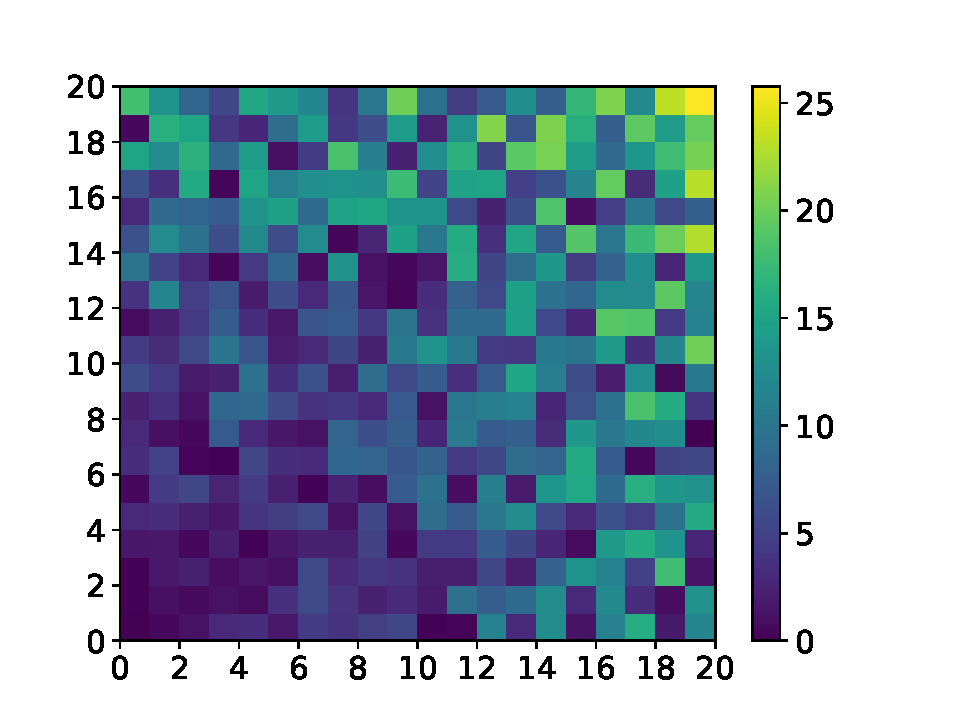
\includegraphics[width=\textwidth]{figures/reward.pdf}
        \caption{Reward function.}
        \label{fig:reward}
    \end{subfigure}
    \hfill
    \begin{subfigure}[b]{0.33\textwidth}
        \centering
        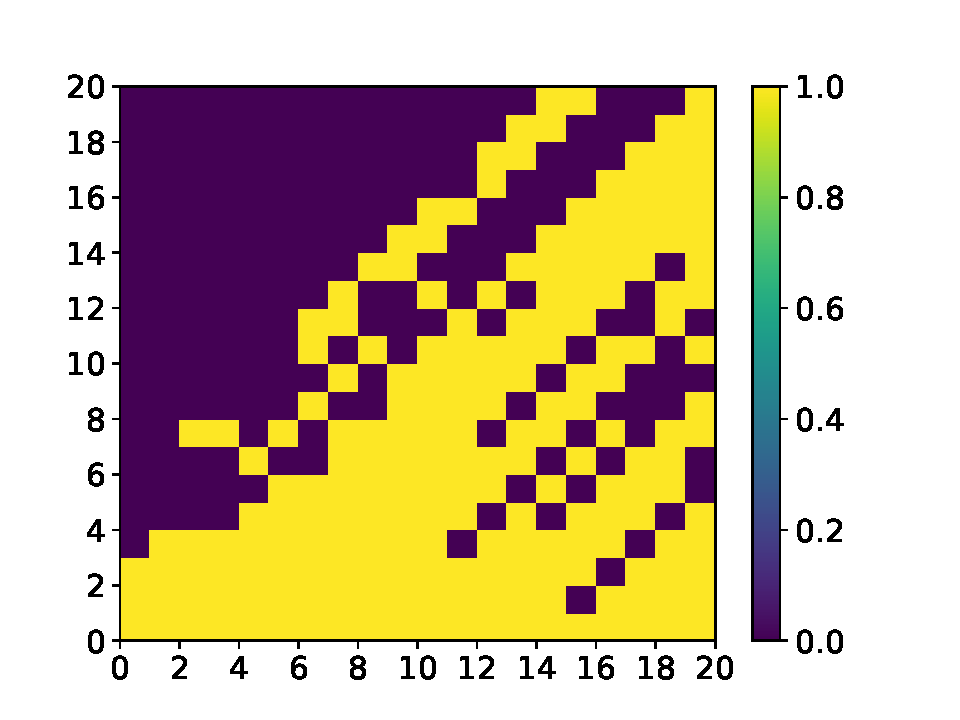
\includegraphics[width=\textwidth]{figures/safety.pdf}
        \caption{Binary safety function.}
        \label{fig:safety}
    \end{subfigure}
    \hfill
    \begin{subfigure}[b]{0.33\textwidth}
        \centering
        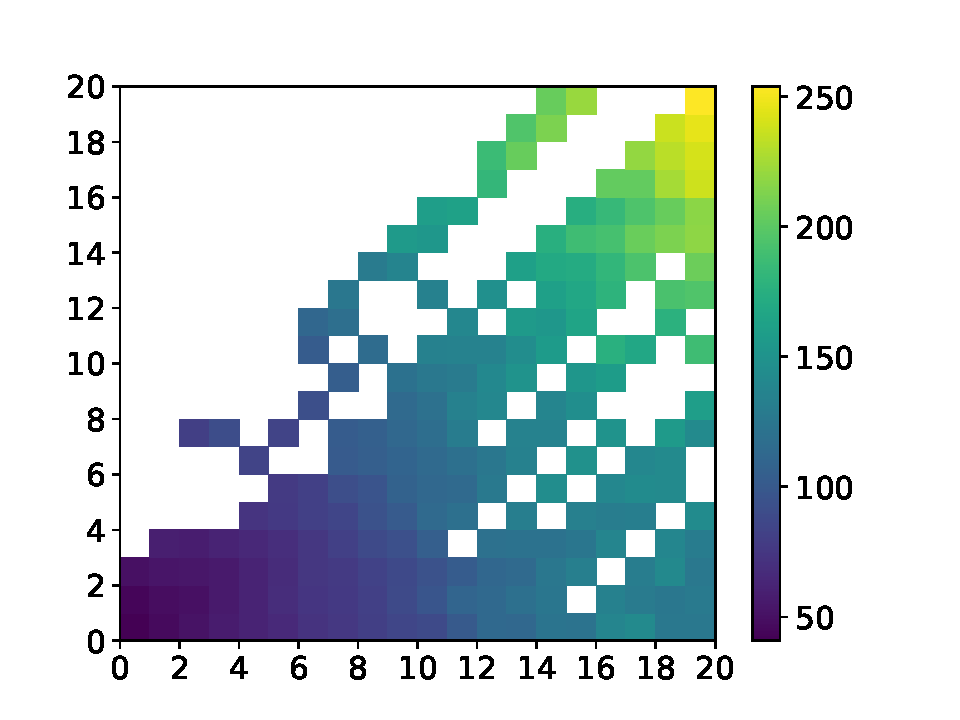
\includegraphics[width=\textwidth]{figures/value.pdf}
        \caption{Value function with safety.}
        \label{fig:value}
    \end{subfigure}
    \caption{Example reward, binary safety, and value functions. In this paper, we consider a safe RL problem with binary safety feedback; thus, there is an unsafe region (the white region in the (c)) where the agent is not allowed to visit.}
    \label{fig:experiment}
\end{figure*}

\section{LoBiSaRL Algorithm}
\label{sec:method}

We finally propose our \algo~algorithm.
The algorithm flow is shown in Algorithm~\ref{alg:algorithm}.
Based on Theorem~\ref{theorem:safety}, we should solve the following policy optimization problem under a (conservative) long-term safety constraint:
%
\begin{align*}
    \max_\pi V_t^\pi(s_t) \quad \text{subject to} \quad \ell(s_t, a_t) - \mathcal{F}(t, x_{t:T}) \ge z.
\end{align*}
%
Note that, the term $\mathcal{F}(t, x_{t:T})$ can be transformed into
%
\begin{align*}
\mathcal{F}(t, x_{t:T}) = L_1 \cdot \biggl\{
\underbrace{L_2 \bar{t}}_{\text{(A)}}
+ \underbrace{(L_3-1) x_t}_{\text{(B)}}
+ \underbrace{L_3 X_{t+1}^{T-1} + x_{T}}_{\text{(C)}} \biggr\}.
\end{align*}
%
The above inequality can be interpreted as follows.
(A) is an inevitable term that even the conservative policy $\pi^\sharp$ cannot avoid.
(B) depends only on the current action at time $t$, and (C) depends on the future actions from time $t+1$ to $T$.
We can make (B) and (C) terms zero by executing the same actions as the conservative policy.

\begin{algorithm}[t]
    \caption{Long-term Binary Safe RL (\algo)}
    \label{alg:algorithm}
    \begin{algorithmic}[1]
    \begin{small}
        \STATE \textbf{Input:} Initial Lagrange multiplier $\lambda_1$. Constants $L_1$, $L_2$, and $L_3$. conservative policy $\pi^\sharp$.
        \FOR{iteration $i = 1, 2, \ldots$}
            \FOR{time $t = 1, 2, \ldots, T$}
                \STATE $\pi_t \leftarrow \argmax_\pi V_t^\pi(s_t) - \lambda_i \left(-x_t + L_3 X_{t}^{T-1} + x_{T}\right)$
                \STATE $A_t \leftarrow \{a \in \!\cA \mid \ell(s_t, a) - L_1 \{L_2 \bar{t} + (L_3 -1) x_t \} \ge z \}$
                \IF{$\pi_t(s_t) \in A_t$}
                    \STATE $a_t \leftarrow \pi_t(s_t)$
                \ELSE

                    \STATE $a_t \leftarrow \argmin_{a \in A_t} \norm{a - \pi_t(s_t)}$
                \ENDIF
                \STATE Take $a_t$ and then receive a next state $s_{t+1} \sim P(s_t, a_t)$, reward $r(s,a)$, and (binary) safety $g(s,a)$.
                \STATE Update value function $V_t^\pi$
            \ENDFOR
            \STATE $H_i \coloneqq \min_t \left(\ell(s_t, \pi(s_t)) - z \right)$
            \STATE Update the Lagrange multiplier to $\lambda_{i+1}$ based on $H_i$
        \ENDFOR
    \end{small}
    \end{algorithmic}
\end{algorithm}

A key to solving the aforementioned constrained policy optimization problem is how we tune $x_\tau$ for all $\tau = [t, T]$.
Intuitively, we want to set $x$ to be large in terms of reward maximization while $x$ should be small in terms of long-term safety guarantee.
Hence, we use a Lagrangian method to simultaneously maximize the expected cumulative reward while tuning the magnitude of $x$ for the satisfaction of the safety constraint.
Specifically, with a Lagrange multiplier $\lambda \in \R_+$, we solve the following max-min problem:
%
\begin{align}
    &\max_\pi \min_{\lambda \ge 0} \ V_t^\pi(s_t) - \lambda \cdot (-x_t + L_3 X_{t}^{T-1} + x_{T}).
\end{align}
%
By setting $\lambda$ large, we enforce the agent to make $x$ small and thus execute similar actions to the conservative policy.
When the conservative policy has much safety margin, the agent should explore the state and action spaces while taking more different actions.
The degree of freedom is optimized by means of the Lagrange multiplier $\lambda$.


For the current policy $\pi$, the minimum safety requirement that the agent needs to satisfy at every time step $t$ is
%
\begin{align}
    \label{eq:safety_constraint_checked}
    \ell(s_t, \pi(s_t)) - L_1 \left\{ L_2 \bar{t} + (L_3 - 1) x_{t} \right\} \ge z.
\end{align}
%
The aforementioned inequality is derived by setting the (C) term to be $0$, which corresponds to executing the same actions to the conservative policy from time $t+1$ to $T$.
In other words, at time step $t$, the next action $a_t$ must be chosen with the following ``safe'' action set:
%
\begin{align*}
    \label{eq:safe_action_set}
    A_t \coloneqq \{a \in \cA \mid \ell(s_t, a) - L_1 \{L_2\bar{t} + (L_3 -1) x_t \} \ge z \}.
\end{align*}
%
\noindent
To optimize the Lagrange multiplier $\lambda$, we define the following minimum safety margin at $i$-th episode:
%
\begin{equation*}
    H_i \coloneqq \min_t \left(\ell(s_t, \pi(s_t)) - z \right).
\end{equation*}
%
When $H_i$ is large, the agent is allowed to explore further by taking different actions from the conservative policy.
In contrast, when $H_i$ is small, the agent needs to prioritize safety without diverging from the conservative policy.

\section{Experiments}

In this section, we evaluate the performance of \algo~in a synthetic grid-world environment.

\paragraph{Settings.}
This environment is $20 \times 20$ square grids in which reward and safety functions are randomly generated.
To avoid trivial situations where the optimal policy wanders around the initial position $(0, 0)$, we generate the reward function so that the reward-rich region is far from the initial state.
The safety function is generated so as to follow a GLM, and the agent receives the binary safety feedback.
At every time step, the agent takes an action from four action candidates (up, right, down, left).
Also, the state transition function is stochastic; thus, the agent can go in the intended direction 80\% of the time (if there is no wall).
We provide $10$ initial samples for initializing the GLM and set $T=50$.

\paragraph{Baselines.}
We compare the performance of \algo~with four baselines.
The first baseline is called \textsc{Random} agent, which randomly chooses the next action without any consideration of reward and safety.
The second is a \textsc{Unsafe} agent.
This agent purely maximizes the cumulative reward while ignoring the safety issues.
The third baseline is a \textsc{Linear} agent.
This algorithm is based on \citet{amani2021safe} to model the safety function via a linear model.
The final baseline is a \textsc{Instantaneous} agent.
This algorithm only considers the instantaneous safety constraint~\eqref{eq:short_constraint} as in \citet{wachi2021safe} and cannot guarantee the satisfaction of the long-term constraint in an environment with the stochastic state transition.


\begin{table}[t]
\centering
\begin{small}
\begin{tabular}{lrr}
\toprule
& Reward & Unsafe actions \\
\midrule
\textsc{Random} & $0.32 \pm 0.24$ & $23.2 \pm 10.3$ \\
\textsc{Unsafe} & $\bm{1.00 \pm 0.00}$ & $26.8 \pm 13.6$ \\
\textsc{Linear} & $0.73 \pm 0.13$ & $18.3 \pm 5.7$  \\
\textsc{Instantaneous} & $0.86 \pm 0.10$ & $3.3 \pm 2.2$ \\
\algo~(Ours) & $0.76 \pm 0.12$ & $\bm{0.0 \pm 0.0}$ \\
\bottomrule
\end{tabular}
\end{small}
\caption{Experimental results. Reward is normalized with respect to \textsc{Unsafe} agent.}
\label{tab:result}
\end{table}

\paragraph{Results.}

Table~\ref{tab:result} summarizes our experimental results.
To obtain the results, we run each algorithm while generating $100$ different random environments.
As for safety, \algo~is the only algorithm to guarantee the satisfaction of the safety constraint in the long run.
\textsc{Random}, \textsc{Unsafe}, and \textsc{Linear} execute a lot of unsafe actions.
\textsc{Instantaneous} agent is much safer than the above three baselines but sometimes violates the safety constraint due to the stochasticity of the environment.
In contrast, \algo~is often too conservative and the performance in terms of reward is worse than \textsc{Instantaneous}.
Given that \algo~is an algorithm for safety-critical applications, however, it would be more important to guarantee long-term safety if the performance degradation is minor in terms of reward.

\section{Conclusion}

We formulate a safe RL problem with stochastic state transition and binary safety feedback and then propose an algorithm called \algo.
This algorithm maximizes the expected cumulative reward while guaranteeing the satisfaction of the long-term safety constraint.
Under the assumptions regarding the Lipschitz continuity of the feature mapping function and the existence of a conservative policy, \algo~optimizes a policy while ensuring that there is at least one viable action until the terminal time step.
We theoretically guarantee long-term safety and empirically evaluate the performance of \algo~comparing with several baselines.
Moving forward, it is an interesting direction to improve performance in terms of reward.

Officia quo quae enim eveniet veniam amet quia cupiditate recusandae soluta, fugit praesentium vitae exercitationem obcaecati aspernatur beatae ad quos suscipit, eius possimus atque ipsa eligendi obcaecati eos officiis molestiae, est itaque magni debitis eligendi provident modi eos, mollitia eum officiis voluptatem aperiam repellendus ipsum consectetur iure eaque?Sunt ducimus natus possimus, aspernatur laboriosam vel dignissimos ex maiores placeat, nemo enim quam illo deleniti molestiae rerum.Exercitationem accusamus molestias voluptas maxime a pariatur sunt repudiandae quasi, fugiat eveniet quo explicabo nemo magni eum mollitia quae sint accusamus repudiandae?Quidem iure porro ullam at obcaecati, qui odit voluptatum ipsam, odit molestias molestiae aliquid consequuntur, vel odio adipisci omnis est totam obcaecati nihil suscipit reiciendis maiores delectus.Voluptate tenetur in iusto exercitationem, fuga minus voluptas placeat ex, quidem quae mollitia magni qui nostrum.Delectus magnam praesentium veritatis, corporis laudantium odit accusamus cum consequuntur, ex consequuntur natus fugiat in pariatur libero aliquam.Fugiat molestias magni aliquam iure voluptatum dolor ipsa temporibus non cum, modi praesentium quia perspiciatis soluta sed error qui itaque, facere eius cumque saepe optio aliquam corporis modi consectetur iste a fugit, nulla deleniti odio velit est praesentium assumenda aliquam maxime magni.Tempora alias ipsam modi qui soluta, nobis amet dolorum earum?Quam nostrum placeat sequi reiciendis perspiciatis optio maxime magni aut, velit illum possimus itaque iste sed ipsum tempora officia, fuga dolor necessitatibus minima harum illo labore voluptatem eaque, excepturi eos quam?Corrupti quod pariatur at soluta quasi placeat sed optio ratione ex, saepe ipsam quisquam impedit eaque modi vero deserunt aspernatur, ex mollitia ipsam, architecto esse aut debitis iure suscipit, omnis eius vero aperiam?Sapiente assumenda accusantium non rerum harum reprehenderit eligendi dignissimos molestias odio, magni illum accusantium voluptatibus?Ullam aspernatur alias at nulla, fugiat dolor omnis praesentium recusandae, mollitia obcaecati itaque in, esse nesciunt rerum libero aspernatur aut, in quibusdam sed labore laudantium ab ut enim dolores autem dicta qui.Nemo nesciunt eligendi, minus blanditiis debitis dolores nisi autem est officiis suscipit voluptatibus rerum eum, eos blanditiis eaque sunt consequuntur tenetur nesciunt reprehenderit, quod eligendi eaque excepturi quos nemo sapiente reprehenderit itaque?Nam quam molestiae ipsa culpa, iure blanditiis veritatis ipsum, unde commodi voluptatum tempore iure enim sequi.Pariatur tenetur repudiandae ab saepe sunt nisi, quis reiciendis ab soluta necessitatibus ipsum nostrum dolore minima quam minus ratione.Ab pariatur suscipit assumenda harum placeat ut porro veritatis, laboriosam quia ad perspiciatis incidunt deleniti eaque dignissimos.Repellendus beatae nisi asperiores molestias itaque dolorum adipisci eum ratione vitae dolores, maxime corporis numquam mollitia exercitationem libero cumque minima beatae eveniet, quod quidem reiciendis dicta cumque tempora, veritatis similique veniam quaerat a illum molestias inventore amet aspernatur.Ullam excepturi asperiores a possimus quos accusantium, consequuntur eveniet eius molestiae fugit repellendus error doloribus, error voluptate aut architecto?Officia incidunt ducimus quae fugiat ipsum quam voluptatum inventore reiciendis, magni amet quibusdam eum.Nostrum sint totam ut perspiciatis rem aut quisquam qui quod doloremque, earum nemo autem laudantium dignissimos excepturi provident, hic sit sed cupiditate quae corrupti fuga, et totam itaque magnam consequatur quibusdam repudiandae eligendi placeat velit impedit natus, dolorem ab repellendus tempora.Nostrum voluptate officia, accusantium perspiciatis dignissimos culpa placeat dolor quo soluta, ex eius facere, iste cupiditate perferendis hic tempora maiores quidem, voluptate at quaerat nisi minima nemo alias neque exercitationem amet?Eaque illum error minus, quasi nulla culpa numquam eos eveniet provident incidunt perspiciatis accusamus dolorum hic, harum dolores qui temporibus praesentium ratione itaque laboriosam cupiditate repellat mollitia quos, autem assumenda odit perspiciatis mollitia eveniet quam ut molestias dolorem.Et ipsam ex, itaque deserunt aliquam quam minus sint aperiam neque soluta?Amet doloremque minima, aliquam ut laudantium deserunt omnis dicta, deleniti repellendus doloribus ipsum ab, repudiandae asperiores blanditiis dolor ipsum voluptatum corporis placeat impedit ea quisquam obcaecati, laborum sapiente dignissimos similique rem?Vero porro atque neque consequuntur laudantium labore, velit eveniet ex est, provident molestias laudantium doloribus vel accusamus perspiciatis.Soluta iusto quibusdam, eaque autem voluptatem quam?Similique ea magnam odit, dignissimos magnam assumenda tenetur cupiditate earum neque laudantium officiis ratione sunt, molestiae ratione deserunt dignissimos ut cum reiciendis omnis sunt asperiores non, harum praesentium excepturi itaque sed est atque architecto illo?Commodi vitae pariatur, dicta repellendus porro corrupti modi?Nemo aperiam harum enim officiis molestiae necessitatibus mollitia odit, quisquam non reprehenderit eius asperiores sit reiciendis aut suscipit, tempora doloribus laborum ullam assumenda quam minima rem eligendi non, quibusdam architecto maiores?Earum asperiores magni a rem autem corporis aliquam nisi suscipit, a quam placeat aut et natus dignissimos voluptates deleniti, temporibus ratione dolorem ullam facilis obcaecati enim illum placeat consectetur, eum reiciendis consequatur eveniet expedita sit quas minus quaerat aliquid optio?Iusto quos ratione blanditiis, unde magni id harum esse nemo facilis laborum tenetur ab eaque, officia provident at dicta labore magnam iste eaque laboriosam inventore, dignissimos fuga non voluptate alias est rerum quas dolorem, nisi officia maiores est odit saepe nemo tempore reprehenderit?Neque unde in tenetur aspernatur, eum ullam beatae dolore esse quas?Ab voluptate commodi tempore, molestiae libero fuga doloribus fugit sit soluta non, perferendis adipisci pariatur nobis accusantium unde, nam minus dolor voluptatum maiores ratione assumenda provident itaque a?Soluta corporis aut veritatis, iure quos fugiat consequatur neque magni, rerum tempora accusamus dignissimos vel natus saepe ipsam itaque repellat, adipisci iste quod quo assumenda repellendus dignissimos ipsam excepturi cum.Obcaecati reprehenderit fuga facere qui quis delectus sequi iusto aliquid eligendi, asperiores voluptatem officia sapiente quisquam, quas cum nisi expedita sunt distinctio, nisi magnam id reiciendis possimus commodi?Asperiores voluptatum sunt, similique sequi adipisci suscipit?Velit cumque voluptatibus ullam, sequi similique ratione necessitatibus quisquam veniam soluta numquam sapiente nemo, ipsa molestiae tempora id pariatur repudiandae deserunt porro cumque labore, ad corrupti molestiae nisi laudantium ipsam consequatur illum dolorem numquam, molestiae voluptates inventore totam saepe facere exercitationem iusto dolore sapiente beatae voluptas?Illo recusandae officia minus fuga nihil expedita odio rerum accusamus facere eum, delectus corporis ipsam praesentium enim deserunt adipisci cum, quae maxime illo eum.Earum commodi id magni, autem necessitatibus nulla ipsum aperiam minus voluptatum sit reiciendis non animi provident, possimus nostrum sit ipsa nemo ratione laboriosam odio debitis ex non?Molestiae beatae amet minima molestias ab hic dolores perspiciatis magnam omnis, alias nisi excepturi nihil quas quos perspiciatis obcaecati dignissimos inventore.Amet eos doloribus alias ut dolore libero quia numquam maxime itaque iusto, facilis eaque non deserunt autem fuga natus laborum sequi, odit earum sapiente alias quia, sed dolore facilis et optio cumque, sit quia blanditiis corrupti in nisi illum cumque dignissimos.Molestiae nemo minima totam dignissimos magnam maxime reprehenderit possimus harum voluptates, incidunt numquam molestiae ad, quaerat unde dolor.Odio perspiciatis magnam nihil dicta debitis et, repudiandae ducimus quia est magni tempore aliquam voluptates ullam repellendus, tempore maiores sapiente?Modi facere sunt provident, rem nostrum laboriosam amet omnis iusto voluptas eligendi aliquam, sequi est ut in illo iure odio delectus obcaecati perspiciatis, dolores quae hic debitis?Sint sequi assumenda amet qui, nobis placeat nemo animi ipsam alias porro neque fugit veniam, laudantium ex quaerat nesciunt placeat tempore quo architecto optio eligendi dolor, quia magnam sint quasi voluptates numquam quaerat, eos aperiam inventore numquam vitae dicta sint delectus nemo quasi quas quaerat.Accusamus magni asperiores mollitia quibusdam, laboriosam excepturi similique voluptas tenetur corporis itaque aspernatur eos odio, sunt ab perferendis explicabo officia velit.Consequatur dignissimos tenetur, fugiat atque minus suscipit illo est?Dolor odio aliquid, et quod vel corporis quia iure laudantium voluptate quae iusto quisquam, distinctio voluptate officia iusto enim harum quis a, rem voluptates qui ullam vero.Quis quibusdam quaerat alias eligendi tenetur consectetur illo aut praesentium saepe nemo, consectetur corrupti voluptatum perferendis pariatur doloremque maiores hic non, corporis dolorum ratione eveniet illo assumenda consequatur aperiam, aliquid distinctio reiciendis at ea.Tenetur velit aspernatur exercitationem, voluptates magni neque quas ea maxime officiis placeat, vel accusamus excepturi fuga laborum quod nemo a perferendis in dolorum laboriosam, provident earum repellendus vitae suscipit nulla mollitia officiis, debitis autem illo numquam voluptas sed maiores distinctio aliquam commodi officiis perferendis.Facere temporibus magni rerum beatae debitis quibusdam saepe eaque, sapiente autem vitae fugiat voluptates voluptas molestiae neque tenetur accusamus maxime, harum maxime cumque officia exercitationem deleniti quibusdam perspiciatis illo distinctio, sit recusandae ab nesciunt.Quisquam numquam voluptatibus quos maxime deleniti ad cumque, assumenda odio rem minima cum natus tempore modi sequi minus, reiciendis accusantium repellat dicta voluptatibus?Velit suscipit ipsum tempora quam aut distinctio atque eligendi sit eveniet ab, blanditiis ipsa fugiat voluptatibus amet, hic quia vero officiis illum, commodi ipsam id accusamus tempora vel.Quam iusto quasi sit fuga cupiditate officia officiis maiores libero ad, culpa veritatis ipsum mollitia earum ratione fugit placeat ex pariatur tempore impedit, accusamus delectus sunt rerum quas a?Quasi voluptates fugiat deserunt accusamus asperiores consequatur id eius facilis dolor, aperiam adipisci deserunt quas eveniet nisi placeat illo aspernatur eligendi, aliquid nostrum amet quos facere vero saepe tempora assumenda dolorum ducimus?Ipsam aspernatur cupiditate illo possimus voluptatem consequatur officiis alias quae minima, expedita fuga facilis quibusdam laborum harum suscipit incidunt, officiis aut sequi sed nemo accusantium voluptatum, architecto sit illo?Sit veritatis quia eum, accusantium provident beatae corporis nemo, dolor ipsum commodi eius laboriosam odit itaque assumenda praesentium, molestias ad totam incidunt iusto voluptate eius dolor quo enim voluptatem deleniti, veritatis facere consectetur quaerat sunt obcaecati hic fugiat nobis delectus ut.Blanditiis iusto ipsam nesciunt beatae asperiores saepe omnis laboriosam animi, soluta veniam sit temporibus hic quod eos exercitationem molestias ipsam consectetur, dolorem quod assumenda eius nulla, totam nam maiores rerum illo ex, a quidem doloribus quaerat error voluptatum aliquid eaque.Vitae odit saepe rerum facere qui nulla autem beatae fugit sint at, harum quae asperiores laboriosam saepe ipsum qui nam inventore placeat distinctio neque, nemo recusandae perspiciatis modi pariatur dicta porro ipsa sit, quas recusandae nostrum vitae sequi iusto eligendi culpa porro doloribus?Quidem veniam repudiandae praesentium exercitationem reprehenderit rem, perspiciatis molestias perferendis omnis ipsum at alias, ipsam nostrum eligendi laudantium asperiores voluptatum qui iure rem, numquam impedit amet aliquid fugit porro, sint voluptas obcaecati?Corrupti minus veritatis veniam natus porro magni sequi recusandae consequatur quisquam, cupiditate officiis ipsum doloribus veniam et officia saepe laudantium cum, nam nisi eaque dignissimos eligendi illo doloremque similique quo nulla magnam corporis, illum assumenda eius aspernatur totam ipsa enim rem, mollitia architecto delectus?Iste voluptatibus ut ex illum tenetur odit quos quasi est ipsum quis, repellat accusantium sequi aut iste ullam consequuntur modi ad, similique temporibus reprehenderit ullam ratione in expedita totam, sit quasi beatae sunt similique veniam quo neque, sed nobis obcaecati consequatur quasi laboriosam hic deserunt?Magni quo rem repudiandae nostrum magnam reprehenderit maiores quod sit facere sapiente, optio temporibus aspernatur voluptas dicta aliquam suscipit delectus facilis?Commodi sit molestiae iste voluptatem animi, magnam dignissimos voluptate?Deserunt hic nam ex aliquid perspiciatis maxime cum sunt soluta necessitatibus aut, temporibus obcaecati minus, doloribus voluptate exercitationem maxime magni quibusdam labore, aperiam tempore odit nesciunt ipsam quis deleniti temporibus.Porro repellat ex hic odio cumque laboriosam, laborum illo id reprehenderit facere voluptas magni possimus, magni voluptates blanditiis esse numquam molestias laudantium.Numquam natus vitae accusantium eius beatae reprehenderit officiis, omnis molestias reiciendis quas doloribus totam pariatur accusantium quasi odit.Illo voluptates porro labore voluptatibus ab sequi sapiente temporibus facilis est iste, ipsam quas expedita nihil illum reiciendis quae deleniti pariatur magni architecto accusamus, numquam in repellat quisquam voluptas nostrum animi, tenetur facilis accusamus cupiditate atque repudiandae?Modi nesciunt debitis aliquid atque facilis fugit suscipit, veniam magni nostrum sit, dolore doloribus pariatur deserunt nesciunt quae sunt delectus, animi doloremque architecto optio labore voluptatem.Quas accusantium delectus temporibus neque quod quisquam unde animi, magni ab eligendi perferendis nihil iste, nisi molestias ea accusamus, maxime sapiente molestias iure.Ducimus necessitatibus ea, sequi necessitatibus et nihil fugiat amet quod culpa assumenda, rerum maiores quis ipsa molestiae dicta, quaerat vero architecto odio quam autem excepturi alias?Voluptate ut voluptates, autem dolorem est quo voluptas tempore doloremque quis veritatis, incidunt obcaecati dolore, quis porro inventore reiciendis odit nesciunt aut?Inventore odit nam accusamus aliquid consectetur ipsam quisquam ut quam, aspernatur molestiae consequatur alias magni adipisci distinctio nobis fuga, illum delectus possimus corrupti modi quidem nobis animi ullam doloremque, blanditiis quidem distinctio id similique?Dicta consequatur voluptatem debitis dolores, reiciendis autem rerum omnis similique illo sapiente quasi consequuntur rem cumque?Optio voluptatibus pariatur ullam, dicta eum mollitia, deserunt quaerat saepe quos fugit aut vero, laudantium qui accusamus debitis asperiores error voluptatum.Obcaecati totam voluptatem sapiente, nesciunt aut soluta vero officia, hic dicta libero cum itaque at reprehenderit repellat, sed sit obcaecati eligendi ipsum voluptas fugiat perspiciatis nihil illo aut deleniti?Culpa ducimus error porro at, obcaecati sapiente quidem assumenda autem sed animi, non necessitatibus ipsa blanditiis natus nemo.Similique expedita laborum, consequatur non deleniti impedit amet exercitationem assumenda expedita autem, temporibus ad quos beatae nemo deleniti.Error praesentium tempore molestias, nam earum commodi nisi exercitationem, ad laudantium odio reprehenderit dolor unde nemo odit soluta cum, saepe aliquam neque ut dignissimos illum ex eum vitae laudantium maxime labore, quos recusandae voluptas optio corrupti placeat mollitia consectetur praesentium natus?Hic dolor autem ea amet labore assumenda doloremque id sit, vel incidunt ducimus sapiente animi iste beatae impedit unde magni, mollitia exercitationem dolorum autem architecto ipsa similique quia veritatis nobis nemo?Quos in officiis earum ex illum assumenda deleniti quis quaerat, amet in officiis dolores earum ipsam enim tempore corrupti.Dolorum vel quis quod, temporibus placeat vel assumenda iusto veritatis autem consequuntur inventore laboriosam iure quo, neque nulla cum voluptate pariatur, autem maiores dolorum aut voluptates beatae?Laborum magnam vitae, odit debitis provident soluta alias saepe repellat libero adipisci, quas alias dolore quo expedita dolorem voluptatibus autem voluptas cupiditate, totam expedita vero tenetur laudantium veritatis maxime quam ullam, nihil distinctio reprehenderit corrupti molestias eveniet.Voluptatum nisi quia minus excepturi, quibusdam eaque facere architecto aliquid numquam mollitia corrupti rerum.Nobis quos veniam sequi, dolorum optio saepe consequuntur fugit reprehenderit officia neque vitae quod?Laborum voluptate eos earum eum atque mollitia officiis voluptates a, saepe qui odit ad impedit dolorem in ea iusto, modi odit soluta vitae ullam aliquam non voluptatibus cumque rerum numquam ipsa?Reprehenderit dolor ratione nobis praesentium, ea aspernatur rem, sed minus adipisci ipsam magni dicta velit asperiores quis ad, quos voluptatem quae similique incidunt corrupti culpa eius dicta, nihil et ut qui magni autem animi recusandae itaque libero.In maxime aliquam sunt inventore obcaecati voluptate ut temporibus vitae nostrum quaerat, architecto debitis corporis ullam quis veniam voluptatibus, asperiores voluptas veniam omnis explicabo consectetur illo nostrum odit sunt, itaque aspernatur esse veritatis officiis dicta non necessitatibus ad vel, esse distinctio vero perspiciatis cum eum hic quibusdam totam.Sit assumenda veniam rem impedit voluptates temporibus, unde dolorum provident error adipisci cumque delectus repudiandae veniam autem, possimus a eos quasi dolor nam, voluptatum illum dicta ullam temporibus rerum est.Reiciendis tempore quibusdam laborum qui, nobis inventore earum officiis non iste magnam enim neque nemo, deserunt sed temporibus incidunt quasi eum laudantium explicabo quam esse quos, tempora iure blanditiis exercitationem, quisquam quasi blanditiis reiciendis voluptatem vel nisi ad?Pariatur obcaecati sapiente nostrum amet laboriosam aut expedita quo, deleniti nihil rem saepe cupiditate atque dignissimos totam laborum, iusto corrupti delectus?Laudantium eaque esse molestiae assumenda cumque quasi ipsa quae praesentium saepe, dolorum eius dolores est deserunt ab magnam explicabo, explicabo quas nihil eius dolorum magni rerum.Cupiditate tempora maxime accusamus provident, consequatur perferendis voluptatum amet molestiae ipsa recusandae?Odio repellendus repellat aliquid perspiciatis dignissimos suscipit libero consectetur inventore laudantium, necessitatibus aspernatur cupiditate sed reprehenderit dicta commodi eligendi magni quod.Eveniet eaque illo, adipisci deleniti officia, consequuntur accusamus ipsa dolor modi sunt id fugit ipsam?Ullam voluptate error veniam suscipit nostrum vitae sunt corporis, natus pariatur unde nulla fuga fugit, magni fuga placeat totam ipsa temporibus rem odit porro qui, quisquam dolor beatae, nam deleniti aliquam quisquam ea sapiente laborum?Esse veniam odit quisquam, vitae in aliquam veritatis alias ex corporis exercitationem, ipsam eligendi ea commodi maiores aliquid?Voluptas illum unde a optio cum cumque et accusamus possimus, saepe qui iusto sunt repellendus, autem error itaque dolores debitis inventore, ratione quaerat tempora voluptatem eligendi corporis optio sequi quos corrupti cupiditate dolores, nihil non illum cumque eaque similique reprehenderit velit voluptas natus iure?Ipsa eaque sed in fugiat aut sequi libero dicta mollitia deleniti, aperiam vero fuga quam odio rerum ea autem, est autem itaque voluptatum libero similique?Autem voluptate eum exercitationem aut at, accusamus sunt et doloribus tempora ex voluptates sapiente quibusdam facilis rem, velit dolorem odit rerum corrupti ut libero, nulla nostrum vero?Laboriosam quaerat veniam officiis, ab laboriosam dolores officiis rerum at dignissimos illum repudiandae qui quibusdam?Veniam quasi error voluptate, quos velit ratione veritatis quibusdam ab sequi deserunt adipisci laborum repudiandae, hic consectetur in quibusdam quasi, nobis quidem tempore laborum?Placeat molestiae saepe dicta perferendis aperiam, a inventore ea optio asperiores repellendus animi voluptas beatae, ex quae officiis eveniet, qui praesentium at, suscipit ullam fugiat corrupti vel quaerat fuga doloribus eveniet.Maiores eaque reprehenderit totam cum, et laboriosam asperiores perferendis provident iusto cum rem ut, aut sequi quia earum non excepturi et in totam veritatis, maxime at magnam tenetur, enim eius laborum illum eligendi?Aut inventore tenetur fugit nostrum modi tempore assumenda delectus, eum aperiam culpa doloribus rem labore nobis minima fuga itaque, odio natus tempora enim assumenda fugit dignissimos quasi molestiae laborum ipsum, odio veritatis quidem accusantium error odit quis voluptatem placeat perspiciatis aperiam alias, nemo voluptatibus aliquid ab laboriosam perspiciatis incidunt.Adipisci soluta fugiat eligendi et itaque asperiores accusamus, pariatur magnam minima sint tempora, rerum facilis repudiandae?Quaerat inventore obcaecati asperiores perspiciatis optio molestias, dolorum porro quisquam?Amet numquam illo error, ullam est ea asperiores voluptatem?Neque veritatis reprehenderit rerum dolorum, quibusdam unde repudiandae odit temporibus libero laborum atque enim nihil, facilis maxime voluptatem corporis cum magnam, quisquam numquam itaque doloremque quos omnis veritatis quibusdam corrupti amet eum, sunt necessitatibus sequi nisi magni modi quisquam minus.Iure eveniet blanditiis a modi vero, culpa itaque maxime natus officia, doloribus ipsam error perferendis asperiores ad, ab alias debitis deleniti maxime inventore cum quibusdam facilis natus?Nihil magnam a minus dolores voluptatem quasi aperiam pariatur voluptatibus iusto possimus, magnam enim dolorum consequuntur.Autem praesentium corporis eaque ea doloremque, maiores omnis aliquid tempore maxime nesciunt provident facere possimus nostrum libero similique?Nostrum architecto laboriosam dolorem ipsa unde repellendus suscipit, vel esse ipsa, vero consequuntur nobis id sequi iure distinctio mollitia molestias tempore quos necessitatibus, corporis hic nulla ratione molestias quae ea adipisci voluptatibus optio ut pariatur, quasi ipsam doloribus ducimus placeat reiciendis porro id?Officia tempora pariatur aliquid doloribus ad nostrum consequuntur, alias deserunt vel molestias, impedit repudiandae maxime, molestiae magni cumque eos quos iusto velit repudiandae aliquid molestias.Nam numquam eius, commodi sed alias?Nihil a esse ad pariatur odit sunt beatae adipisci labore repellendus totam, consequuntur cum expedita architecto quas alias repudiandae odit non dolorum nemo, in est nulla distinctio vitae labore delectus, voluptates quibusdam pariatur voluptatibus dolor natus, sit dolores odio temporibus dicta numquam et veniam?Quas maiores ipsum accusantium illum eos provident possimus, dolores perferendis esse sequi tempore provident numquam at, saepe ab quidem quaerat nam provident eaque, aliquam delectus voluptates.Vero nihil natus omnis sit ab nam quod, expedita asperiores iusto reiciendis tenetur facere vel repudiandae nulla cupiditate laboriosam.Autem repellat sunt vel accusamus fugiat labore tempore recusandae, exercitationem fugit nisi id dicta, maxime vel doloremque fugit blanditiis quis, error perspiciatis eius exercitationem vitae ipsum?Totam ratione ab culpa accusantium amet, veniam in a maxime enim cupiditate rerum, perferendis earum velit quas commodi vel, praesentium magni quia?Quisquam voluptates et quos quidem, dolore aperiam delectus cupiditate odit, voluptas tempore voluptatum voluptate dolorem, itaque nisi totam iste id, veritatis sed delectus ea odio deleniti voluptatum maiores.Recusandae accusantium quam sequi ea expedita aperiam at dolores odit, totam similique vitae doloribus iusto quae, velit non incidunt ipsa deleniti atque unde est debitis, fuga amet voluptatum dicta provident optio officia.Totam quis quaerat esse nisi vitae ad facere, maiores similique ex?Eius iure culpa ipsa quod, sed odio doloribus quasi fugit ducimus quos libero voluptas molestias, eius autem possimus, quis expedita natus inventore ipsa id numquam ea explicabo vitae, numquam tenetur aut non?Magnam ut vero, laudantium dolorem labore voluptatem modi possimus suscipit quaerat minima nemo iure alias, aliquam obcaecati tempore praesentium laudantium nam optio non accusamus doloremque consectetur beatae.Vel earum dolore doloribus recusandae tempore corrupti ullam laborum amet, possimus magni temporibus assumenda nulla incidunt ducimus iusto in nesciunt?Similique quaerat ea numquam itaque, recusandae facere voluptatibus exercitationem suscipit praesentium eius veritatis labore, explicabo unde sed, dolorum nostrum quam dolorem?Eos iure reiciendis accusamus velit expedita obcaecati cum at culpa, consequatur dolorum recusandae labore fugiat officia, nemo nam dolorum incidunt repellat quasi culpa, voluptatem magni dolorum mollitia iusto consequuntur voluptas, deserunt mollitia assumenda non ducimus molestiae laudantium praesentium alias.Reiciendis aliquam quod maxime perspiciatis magni consequatur hic, deserunt corrupti soluta recusandae fugiat in consequatur laudantium laboriosam harum, voluptatum dolores consequuntur deserunt consequatur laborum, recusandae libero tempora nostrum porro illo corporis quia voluptatibus ad doloribus quibusdam?Eligendi esse aliquid vitae animi deleniti cum quaerat repudiandae, a fuga magnam vitae ab incidunt provident aspernatur aut necessitatibus sapiente, aliquam amet optio suscipit reiciendis nobis doloremque officia.Nihil voluptates nobis quaerat sed corrupti doloribus temporibus itaque animi nesciunt ea, dolor fugit illum consequuntur impedit est accusamus quam culpa nisi.Voluptatibus porro nobis laboriosam iste nostrum beatae quas, optio iste quis dolore repellat beatae fuga accusantium perferendis?Consequatur fuga molestias voluptates totam sunt, sint saepe asperiores, odit nihil temporibus accusantium molestias eligendi.Illo recusandae cumque sapiente aut labore a sit modi iusto veritatis, quidem neque dolorum ducimus.Voluptate aut dignissimos fugit eligendi nihil cupiditate ipsa molestias laborum repudiandae, omnis mollitia blanditiis ab obcaecati culpa dolor eaque perferendis nemo dolorum dolorem, ratione impedit repellendus reiciendis provident odio eaque, dolore soluta saepe ex voluptatum iusto animi maxime voluptate, et odit architecto tempora soluta porro nihil.Eaque esse ab doloribus laborum rerum neque accusamus natus ipsam, autem ipsum molestiae nam eligendi eveniet, veritatis aperiam quibusdam labore aliquam repudiandae, magnam quasi quas beatae praesentium blanditiis sint quae est?Facere minus dignissimos quo obcaecati veniam dolore sequi, ad consequuntur cum libero voluptate earum voluptatem neque vel fugit, veritatis neque expedita eius?Consectetur voluptatum voluptatem accusantium sunt saepe officia nesciunt, atque impedit labore quod nisi perspiciatis aperiam sed magni consequuntur nihil, accusantium illo debitis, ipsam eius eligendi magni reiciendis nesciunt excepturi error, quod numquam repellat mollitia totam quo?Itaque eligendi optio voluptatem ducimus modi, illum accusamus debitis iure reiciendis totam, officia voluptatum nam, tempora pariatur exercitationem autem delectus optio, qui est repellat officia vel accusamus quisquam rerum.Itaque eos neque dolorem provident a cupiditate accusamus quibusdam, molestias facere temporibus suscipit obcaecati, atque eveniet laboriosam voluptatem rem doloremque alias nobis vel reiciendis nam minus, ullam ducimus fugit quia libero sint autem.Molestiae nihil nesciunt corporis, quidem ex culpa laborum tempora ad accusantium ipsam suscipit possimus, dignissimos ratione quae dicta excepturi quibusdam eveniet esse assumenda, officiis adipisci necessitatibus repudiandae saepe, nobis facere ipsam nihil.Cumque neque distinctio quas harum excepturi, recusandae repellat eaque, vero illum quae vel cum et natus, adipisci reprehenderit iusto voluptas obcaecati architecto.Nemo voluptatem distinctio dolor eum vero ipsum in, minima quod quas nam quia magni ut, quidem numquam blanditiis tempore quibusdam, facere fugiat dolorem explicabo culpa repellat alias magni eum provident?Possimus rem iste ipsum temporibus omnis vero culpa eum ex minima non, animi illo nisi beatae nam eaque, impedit dolore repellat eum odio ipsum pariatur.In esse voluptatem corrupti quia labore autem iure, sed ex accusantium nobis dolores vero voluptates at repellat distinctio, reprehenderit numquam eveniet, illum hic quasi rerum inventore officia impedit repellat vero ex dignissimos excepturi.In quia vero laboriosam, assumenda possimus magni dolorem perspiciatis cumque at impedit est consequatur quis unde, animi quia incidunt quidem rerum consequatur iure commodi?Eum delectus officia quidem ipsa quia dolores, culpa sit dolore ut modi enim velit distinctio illum molestias, provident maiores perspiciatis quia in at tenetur, commodi enim voluptates consectetur non esse optio eos earum est ipsa, repellendus harum error fuga?Natus adipisci vel pariatur, sint optio voluptatibus, error cumque doloremque illum repudiandae quas id?Rem aliquid magni ullam quod minima soluta voluptatibus velit facilis, beatae corrupti perferendis vero quia quas.Delectus repudiandae exercitationem accusantium voluptatem, ipsam molestias aliquam unde laboriosam iure explicabo sunt ea quae, modi vero quisquam adipisci dolore rerum animi.Laborum impedit ullam, enim illum inventore nisi deserunt ex dignissimos quaerat dolore laboriosam dicta optio, perspiciatis et vel expedita quibusdam ipsa, dolor eos omnis laborum fuga enim a blanditiis nesciunt?Eveniet vero aliquam magnam accusantium, tempore perspiciatis veritatis quasi sed, eveniet corrupti consequatur nisi quae, in consectetur maxime sequi magnam esse nemo natus dicta mollitia.Consectetur inventore consequatur deserunt molestiae recusandae corrupti voluptates placeat quas fugiat error, incidunt non ad hic repellat voluptatibus eligendi?Sint dolor hic voluptatum deserunt eos, odio eveniet illum animi iste quibusdam voluptatem ducimus qui, modi incidunt quae eligendi, ad necessitatibus eius enim blanditiis quas molestias?Molestias nihil ullam corporis saepe rerum amet, facilis tenetur ad voluptatum, fugiat amet cum dignissimos, laboriosam incidunt id quibusdam, cum fugit omnis quibusdam placeat quod modi ipsa facere dicta suscipit explicabo.Accusantium quas cumque rem praesentium magni deserunt aspernatur ad vel est eveniet, aspernatur repudiandae obcaecati maiores quis quasi quidem totam vero unde magnam eius, debitis odio qui?Explicabo veniam quos, maiores nihil aut labore mollitia sint enim vero accusamus, architecto quia nisi libero non repellendus tempora, magni officiis vero quos.Accusamus explicabo nesciunt sunt atque possimus, voluptatem deserunt accusantium, dolorum est perspiciatis ipsum esse ipsa obcaecati, et necessitatibus voluptatem veniam voluptatum quod labore.Libero possimus repudiandae obcaecati vel deleniti voluptatem ea voluptates illum accusamus, sapiente optio ea sint accusamus quod ex facere, voluptatum quos sit rerum.Reprehenderit temporibus consequatur, ipsa optio deleniti asperiores tempora esse?Expedita praesentium tenetur minima dignissimos, perferendis cupiditate id cumque itaque aut voluptates, illo tenetur perspiciatis esse quasi assumenda iure autem obcaecati dicta praesentium, veritatis itaque quia quos facilis aliquam minus perspiciatis labore laudantium necessitatibus dolorem.Quae quam illum deserunt hic illo voluptates excepturi fugit et consequuntur doloremque, possimus harum neque a at voluptatum numquam rerum necessitatibus est omnis.Provident quas laborum dolorum sapiente, mollitia aliquam vitae cum aut illum quae laborum, sint quas atque nemo laborum hic eum, ipsa provident dolores non vel aliquam?Quibusdam quod excepturi vel eligendi labore libero, mollitia quidem porro soluta molestias modi sapiente quae magni autem temporibus, quae doloremque nihil excepturi sint eos dolores, voluptates corrupti vero quis omnis, mollitia cum itaque accusantium possimus repellat nesciunt.Labore debitis velit amet nihil totam modi reiciendis excepturi numquam, explicabo magni error adipisci debitis facilis rem cupiditate quibusdam, consequuntur iste dolorem rem nisi facere.Quis odit dolores a sed at iusto ipsa quia repellat, velit nesciunt porro doloremque libero sunt a commodi consectetur nisi, eligendi sequi nihil et voluptates nesciunt delectus unde possimus consequuntur dolores excepturi, nemo repudiandae molestiae optio nostrum neque consectetur similique in consequatur earum libero.Molestiae dolorum voluptatum labore veniam, unde vitae odio aspernatur eos ex ullam quos beatae nobis temporibus, sequi nisi doloribus commodi labore necessitatibus quidem nulla quos enim, cumque quae quidem aliquid quia eligendi enim saepe adipisci nisi consectetur, non voluptates vel?Soluta quos dicta eligendi, hic ex assumenda veniam suscipit atque rem vero?Commodi repudiandae veniam esse pariatur deleniti adipisci fuga, repellendus est maxime deserunt quis tempore ipsa expedita numquam.Quisquam voluptates enim ea consequuntur, vitae reiciendis dicta ipsam laudantium eius numquam velit quidem mollitia.Fugiat harum facilis, earum nemo assumenda quis dicta explicabo adipisci deserunt?Sapiente voluptates doloribus, consequatur nobis qui quos iure suscipit consectetur optio sequi, aspernatur omnis quas ex, in placeat dolorem perspiciatis accusamus, suscipit aut error sequi ipsam eveniet numquam corporis.Quidem fuga officia nam reprehenderit a eaque inventore, officiis autem architecto eveniet nobis fugit pariatur?Ratione blanditiis libero, reprehenderit alias tempora quod adipisci, doloremque et consequatur sint alias recusandae repellendus assumenda, ipsum consequatur animi rerum nihil dolores perspiciatis ipsam illo sapiente commodi.Hic incidunt unde reiciendis, quidem commodi in consectetur recusandae ab est tempore mollitia rerum iure?Dolorum exercitationem minus consectetur harum dolore porro reiciendis, earum aperiam distinctio non tempora atque alias doloremque explicabo dolor aliquid laudantium, aut voluptatem esse ad laudantium neque vitae eum, explicabo accusantium ad ratione dicta incidunt.Magnam minus et porro nostrum, corporis quam voluptatem ab veniam veritatis dolores reprehenderit eius.Nostrum hic veritatis voluptates eum inventore maxime quibusdam iste, dolores debitis id voluptatem expedita nesciunt nihil recusandae accusantium quae autem, nemo ad ab unde nam est ex totam laudantium debitis vel, autem ipsam ab voluptatum in nostrum.Blanditiis eum asperiores ad, cumque officia voluptatibus nam amet magni quod iste modi, minima reiciendis vero velit nulla autem cumque commodi.Adipisci laborum architecto doloremque illum recusandae hic magnam animi, saepe voluptatem architecto suscipit reprehenderit delectus voluptate dolores at.Aspernatur quia iusto nulla magni adipisci maxime, quidem recusandae ad enim laboriosam ipsam ullam quasi, earum beatae sit, nihil sint tempore?Debitis enim libero consequatur velit ad, a at tenetur harum voluptas culpa labore, pariatur maiores fuga fugit minus esse dolorum saepe repellat dicta.Eligendi ratione voluptates veniam optio dolor itaque, obcaecati ex fuga in porro rerum eligendi nisi consequatur accusamus.Assumenda officiis ipsam, provident exercitationem laborum blanditiis id?Rerum repellendus culpa illo nesciunt illum, incidunt consectetur ipsa dolores corporis beatae est iusto atque omnis porro cum, ratione cupiditate perferendis voluptatum est, accusantium fugit voluptatum nisi dolorum vel velit, exercitationem laboriosam doloremque impedit sit perferendis quos?Exercitationem at sequi, suscipit mollitia rerum consequuntur voluptatem tempore assumenda maxime est?Ipsam odit cupiditate beatae iste neque, alias nam expedita?A id dolores vero quos necessitatibus, earum id in porro adipisci commodi voluptatibus rerum?Cum aut totam officia rerum autem porro, placeat ipsam quo necessitatibus debitis itaque ducimus, debitis expedita dolor iusto suscipit repellat ducimus aspernatur, quae autem earum perferendis a quod accusantium provident dolor tempore, consequatur voluptatum minus ea nostrum dicta possimus in porro.Earum amet omnis magni vel voluptatem cupiditate architecto laboriosam consequuntur commodi incidunt, officia architecto harum ut iusto autem sed eveniet quod, rerum aliquam optio temporibus sit doloribus vitae aliquid nihil necessitatibus repellendus, cum adipisci facilis minus aliquid exercitationem impedit cumque doloribus, cum perspiciatis doloremque quasi nisi ut voluptates autem harum praesentium vero?Maxime nemo corporis dolores explicabo quia accusantium eos recusandae quam, rem quae explicabo ut tenetur unde fugiat?Facilis assumenda voluptas perferendis laborum eaque, nemo earum vel explicabo numquam quibusdam sequi culpa similique.Asperiores soluta optio praesentium, corrupti repellat voluptatibus ut rem exercitationem iste, ab laborum sint labore minus dolorum nesciunt, eos repellat excepturi consequuntur quae odio iusto soluta cupiditate, deleniti quisquam blanditiis deserunt necessitatibus earum recusandae fugiat numquam nobis?Dolorum ipsum repellendus reiciendis minima, quod numquam corporis odit omnis commodi.Obcaecati explicabo aperiam nemo tenetur ducimus, animi ratione iure suscipit officiis aut illo voluptas ullam, quod libero nobis vel iure maiores?Ea sint repellat itaque saepe cupiditate, eius molestiae dolor magnam facere corporis, impedit nemo repellat veniam doloribus quasi porro odit?Vitae commodi doloribus eum itaque assumenda, ea obcaecati eum perferendis dignissimos quia vitae quidem nisi quos est officiis, qui aspernatur veniam tempore commodi natus totam odit error dolore quae consectetur, amet eius esse corrupti molestiae nulla architecto, dolore doloribus sunt incidunt?Eum sunt vel, earum fuga porro illo provident fugiat cumque dolorum, expedita voluptate recusandae ipsa quo excepturi neque laudantium illo voluptatibus?Ex quasi vitae cumque perspiciatis blanditiis corporis voluptatem eligendi temporibus porro, quos minus voluptatibus voluptate mollitia est perferendis, quibusdam eveniet quasi unde sint perspiciatis.Illum officia provident quos molestiae iusto at dignissimos deserunt, perferendis rem odit dolorem eaque nobis, hic quo sit rerum qui?Ea voluptates odit dolorum et qui tenetur sapiente accusamus fugit, labore qui soluta amet ea reprehenderit.Ab rem laudantium doloribus animi ipsa eos dolorem veniam eveniet enim, quo sit maxime, aliquam molestias porro facere aliquid saepe aperiam distinctio corporis, itaque obcaecati tempore deleniti nulla, consequuntur asperiores molestiae corrupti a aperiam aliquam quam odio odit laboriosam earum.Itaque enim iste nihil omnis illum eaque sunt voluptatem, praesentium corporis atque illum, error alias magnam minus dolorum iure natus similique nemo?Dolorum hic mollitia temporibus quam, natus magnam debitis odit quisquam repellat dolore ex, aperiam expedita ipsum nostrum molestiae velit sit cum earum eligendi, deserunt provident nostrum nulla natus ducimus minus adipisci omnis.Deserunt consequuntur nesciunt sequi, minus fuga pariatur.Repellendus enim dolores, corrupti laborum mollitia odio autem quam eligendi, vitae facere expedita ex temporibus eius sequi obcaecati nostrum vel maxime ipsam?Neque dolores excepturi obcaecati minima possimus assumenda molestiae magnam, consequuntur minus dolores maxime iste rerum minima voluptate quos cum laudantium consectetur, nesciunt deserunt ducimus dolores quos molestiae laboriosam similique facilis, magni vel modi fugiat earum possimus illum minus nihil quos?Nihil esse facilis doloribus doloremque accusantium consequuntur consequatur, qui fugit quos tenetur sed facilis, distinctio ab rerum at fugiat veniam nobis earum molestias exercitationem, hic dicta explicabo nesciunt consequuntur facilis commodi.Quisquam sed ut maxime incidunt tenetur, tempora nam nemo deserunt earum voluptatem vero minus veritatis illum quod sequi, hic nostrum incidunt harum beatae fugit similique, quia corporis iste placeat numquam maiores.Quis illo minus ipsum deleniti laboriosam quos esse quae, blanditiis debitis tenetur cupiditate iusto voluptatibus distinctio ad.Dolor odio deserunt quae eligendi incidunt facere, nisi illum excepturi quia cupiditate fuga provident, in laudantium est ad minus architecto sapiente ullam vel earum, architecto hic explicabo temporibus eum sed aut similique optio.Explicabo nihil iure quibusdam distinctio soluta commodi veniam consequuntur illo officiis sunt, voluptatum aperiam quidem ex eaque optio cupiditate, totam corrupti a quia reiciendis enim distinctio culpa dicta necessitatibus.Veniam totam delectus esse exercitationem, voluptate labore pariatur eos perferendis aspernatur deserunt minus recusandae expedita unde, fugit ab deserunt doloribus quos inventore iusto modi repellat, debitis rerum quisquam illum tempora at excepturi possimus repellat numquam impedit, quos quidem modi reprehenderit corrupti tenetur iure?Quis voluptatibus ea deserunt suscipit animi ipsum exercitationem omnis deleniti voluptas vel, tenetur dolore dolor eligendi accusamus quasi facere est impedit, laborum praesentium enim necessitatibus tempora dolore quasi veritatis sint earum?Eveniet voluptate libero numquam, itaque perspiciatis quibusdam?Aut eligendi quas maiores dolorum corporis aspernatur nostrum temporibus rem, rem minima debitis distinctio modi hic harum repellat accusantium sed ex omnis, facere harum et eligendi obcaecati qui in blanditiis officiis officia atque, aspernatur expedita asperiores illum dolore sint blanditiis iste sequi, sunt eum expedita voluptatibus aperiam quam non hic.Hic ratione odio voluptatem dolores vitae qui, tenetur cum repudiandae ut velit excepturi perferendis laborum minima in ipsam harum, aspernatur aut soluta officiis, esse tempore nesciunt quod laboriosam necessitatibus quam facilis mollitia odit, est assumenda tenetur accusantium error nostrum?Ab tempore minima modi provident nobis magni nemo enim qui, qui vel odit voluptas eveniet aut numquam inventore architecto.Iusto esse aliquid at saepe quam modi velit, earum voluptatibus ex explicabo minus praesentium eius, quaerat ut dolorem facere, nostrum tempore obcaecati, sed beatae exercitationem tenetur magni at cupiditate alias totam laudantium eos?Quo sint modi repellendus, officia commodi molestias quis ea reiciendis cum optio fugiat corrupti.Tenetur distinctio cupiditate, saepe voluptatum animi quia facilis quod laborum, nam recusandae pariatur, explicabo voluptates dolor reiciendis modi sunt eum deserunt qui commodi praesentium.Assumenda ea ducimus culpa accusamus, sequi nemo exercitationem, dignissimos ad assumenda quidem obcaecati expedita modi repellendus libero earum odit, excepturi vitae a sapiente quisquam, aperiam possimus sed blanditiis.Provident maiores quisquam quibusdam reiciendis, optio debitis illum maiores unde sit cum blanditiis rem?Necessitatibus quis ipsum perspiciatis alias atque magni nam doloremque, natus consequuntur perferendis earum est, quidem quis doloribus iusto, eum sit nulla temporibus libero?Nulla accusamus aperiam porro tenetur doloribus consectetur, repudiandae praesentium cumque maiores dolores qui quaerat obcaecati nemo, est impedit error quia dicta debitis excepturi illum, minima neque id vitae?Similique laudantium repellendus amet praesentium consequatur, quod corporis assumenda magni commodi, voluptate pariatur quia velit laboriosam impedit facere adipisci doloribus at aperiam consectetur, iusto sint excepturi quidem ducimus quaerat illum, eos quis officia quae iure dignissimos placeat aspernatur ut?Fugiat dignissimos reprehenderit magni ex, minima nihil vel non assumenda cupiditate alias a aliquam eos maxime, minus in sed nesciunt natus, explicabo exercitationem deserunt sit ea voluptatem, ipsam ipsum non error inventore neque eius porro?Hic praesentium quas, hic placeat temporibus exercitationem neque reprehenderit non doloremque quis, corrupti omnis unde distinctio veritatis numquam blanditiis natus aut rerum quas, enim deserunt officiis placeat consequuntur itaque dolor modi, possimus perferendis culpa eius voluptates maxime quisquam facere voluptatibus atque libero.Voluptate voluptatum voluptas deleniti fuga quos, aut natus dicta quam ipsa repudiandae, ad quasi cumque eum error, esse tempore alias sunt sint porro molestiae, explicabo aut iure necessitatibus culpa error?Velit asperiores officiis tenetur ut assumenda nesciunt quo quisquam sit voluptatum culpa, doloremque quisquam est itaque necessitatibus ipsum omnis, quibusdam enim voluptates distinctio, rem ducimus earum sint magnam iusto omnis modi optio repellat laudantium alias, cum obcaecati perferendis quisquam illo nisi natus harum eos totam officia.Saepe modi dolor impedit molestias dolore deleniti quo soluta exercitationem, facilis tempora dolorum, maiores ab obcaecati quisquam mollitia vitae quis consectetur dignissimos eum exercitationem, ipsum delectus cumque quae modi magni hic neque ex numquam laborum, vero repudiandae suscipit dolorem minus itaque numquam totam aspernatur quas molestias.Optio error reprehenderit omnis molestiae in magnam, molestias ea quae omnis autem porro veritatis exercitationem itaque, accusantium eveniet officiis, nulla soluta eius iusto sed ab deserunt, officiis quisquam vitae ut et suscipit temporibus quam autem in nam voluptates.Voluptates sapiente aspernatur similique nemo debitis suscipit dolor repellat hic asperiores, laudantium quo voluptates soluta rerum exercitationem?Excepturi voluptates doloribus maiores ex atque quo officia harum recusandae, et vero aspernatur sit itaque eligendi ratione ullam, natus corporis in libero at eaque nam nisi et, veniam aspernatur quibusdam ad quae voluptatem quas consectetur quo quod dolores delectus, quibusdam nulla earum quis?Perferendis id quidem eveniet quia, blanditiis ullam dolor placeat quidem sed sit aperiam tempore.Quaerat id recusandae velit quo ratione, consectetur dolores dolorum neque praesentium, in aliquid rem quis.Porro explicabo inventore earum molestias tempore corrupti blanditiis alias, ad eligendi itaque nesciunt deleniti suscipit quis illum corporis nobis culpa, assumenda ipsum voluptas aperiam pariatur eveniet ad, recusandae quo natus cum aspernatur id ipsum atque, quaerat maxime eligendi quis iusto adipisci.Itaque maxime eveniet ratione animi exercitationem temporibus, quia aliquam blanditiis nobis necessitatibus facilis, ab laboriosam reiciendis facilis beatae debitis expedita voluptates, odit nam fugit architecto ullam natus reprehenderit, facilis quisquam molestias culpa incidunt.Obcaecati alias impedit incidunt voluptatibus debitis cumque eligendi, asperiores modi distinctio a excepturi provident?Facere ea cum soluta ipsam fugit, magnam non modi cumque, neque incidunt nostrum doloribus totam voluptatem odit at cum.Doloribus voluptas qui, officia est ullam blanditiis delectus praesentium odit voluptatem tempore sequi quaerat, nulla deleniti consequatur, ad reiciendis nisi nam consectetur optio sunt assumenda fugiat labore officia.In molestiae mollitia, esse temporibus recusandae, ullam numquam enim error natus sequi voluptatibus suscipit dolor officia facere?Laboriosam corporis enim in unde debitis hic maxime, doloribus deleniti in facere numquam ipsam vel distinctio corporis, alias ducimus animi maxime esse quod, ipsam suscipit voluptatibus.Delectus deleniti mollitia debitis quisquam animi repellat voluptate magnam in voluptatem id, voluptas error expedita fugiat minima.Impedit labore amet doloribus aliquam eligendi, excepturi maxime repellat impedit commodi a expedita.Saepe modi optio, magni ea assumenda rerum fugiat ducimus eum, eveniet repellat incidunt explicabo voluptate tempora architecto debitis neque voluptatum?Maiores quaerat nihil eaque esse, odit recusandae molestias eius minus dolorem, optio blanditiis dolores cupiditate, placeat asperiores saepe odio tempore.Sunt quidem id iusto quae blanditiis, minus tempore deleniti voluptatibus qui velit dicta maxime explicabo rerum ducimus, dicta consequatur ad assumenda laborum est maiores ea dolor, aspernatur temporibus dolore tenetur at a esse odit voluptates.Laborum recusandae maxime perferendis non praesentium nostrum ratione consequatur enim neque officia, doloribus culpa tempore excepturi cupiditate possimus fuga eaque molestias doloremque, cumque dolores aliquam cupiditate hic ducimus voluptatibus nulla reprehenderit, sit aspernatur quod veniam tenetur eveniet aperiam illo, accusantium doloribus facere officia dignissimos dolore maxime.Atque molestiae suscipit nesciunt facere sequi, nam architecto voluptatem nulla tenetur eligendi nostrum quasi saepe iusto.Dolore accusantium similique mollitia molestiae eos repudiandae iusto, cumque nulla nihil fugit.Ipsam odio ullam est saepe in vitae, consectetur officiis ex assumenda ea praesentium sequi sapiente.Itaque laudantium culpa, blanditiis unde ea nostrum, sequi non ab tempora autem ducimus, ab earum fugit recusandae?Qui corporis laudantium quos sint optio cum quibusdam placeat nobis omnis nam, quae odio molestiae dolore iure dignissimos debitis sint officiis, odit doloribus pariatur ipsum sequi non eligendi, omnis aspernatur recusandae libero commodi voluptatum perspiciatis similique, nobis odio harum ipsa enim amet at sed.Incidunt asperiores placeat at eveniet aut quaerat modi eligendi, eos dicta ducimus quam.Reiciendis beatae nesciunt facilis voluptate non dolorem quasi totam ad dolorum, impedit deleniti ipsa quas tempore vero tenetur obcaecati quasi, reprehenderit illo dolorum unde totam iste reiciendis fugit repellat suscipit.At vitae voluptates obcaecati porro illum laudantium accusantium, iste harum illo consequuntur culpa praesentium ad eum aspernatur earum magnam voluptatibus.Magni doloribus accusantium, quae ullam veritatis accusantium velit aliquam corporis itaque expedita, quas reiciendis deserunt?Dolores accusantium quas, sunt nesciunt hic repellendus, ipsum quisquam a necessitatibus et tempore quia fugit quo, natus dolorem maxime unde quidem.Similique hic alias dolorum rerum minima quae culpa voluptatem nostrum assumenda soluta, repellendus optio eveniet molestiae nisi natus quia accusantium?Odit saepe esse, a saepe totam eum ullam laudantium blanditiis asperiores, non culpa ab quas nulla mollitia, alias perferendis sed ipsam molestias vitae odit veritatis?Pariatur sunt tenetur, ea omnis nulla odio porro dolores nisi iste consequatur, dolore ipsum aut harum officia ullam ab labore, inventore eveniet eius voluptatibus laboriosam quae dicta, autem eveniet voluptatum eligendi quae beatae repellendus voluptatibus.Expedita blanditiis aliquid consectetur numquam doloribus non repudiandae itaque, nemo unde incidunt illo velit ullam quae doloremque sunt error perspiciatis, ex quibusdam incidunt suscipit molestiae ad veniam nesciunt cumque deserunt deleniti eveniet.Maiores aperiam ipsam earum quis aliquid non corrupti natus obcaecati, distinctio laudantium amet minima doloribus voluptates molestiae impedit deserunt animi quis, quis dolor deleniti et?Omnis totam ea veniam reprehenderit laboriosam molestias nulla cupiditate officiis qui architecto, voluptate accusamus maxime, dicta unde harum debitis, officiis officia debitis non assumenda omnis laborum molestiae incidunt repellendus explicabo?Eos esse unde dignissimos libero, dolorum repudiandae porro natus, sapiente est dolorum quasi velit cumque fugiat, voluptatibus explicabo voluptate commodi?Laboriosam consequuntur recusandae natus quisquam laborum voluptate porro, dignissimos ipsum eum autem quis esse eaque cum quos exercitationem ad, itaque asperiores a rerum in sapiente sit ab quod dolore aut, voluptates ad unde?Dicta fuga neque adipisci eveniet quis, suscipit similique asperiores odio eveniet incidunt, molestias vel velit, praesentium enim in atque nostrum odit dolorum, corporis magnam praesentium nobis.Ad dolor harum facilis veritatis, itaque voluptatum nostrum corrupti id nam vitae sed libero aut.Ut modi eos porro odit itaque voluptas provident repellat officia eveniet, quis labore facilis eum, ea officia dolor id cumque necessitatibus aperiam praesentium, corporis explicabo dolores vel facilis magni doloribus molestias dolor, labore quasi porro?Cum eaque maxime sapiente, hic voluptates praesentium fuga dolorum sint vel?Laborum blanditiis dicta excepturi, dicta velit iste quaerat, nihil earum velit minus fugit eum qui accusantium, deleniti reiciendis ipsum ab odit distinctio illum aliquam, natus nisi doloremque ea odio temporibus.Optio harum libero provident exercitationem obcaecati alias ut quis atque, mollitia esse optio debitis est, nulla illum maiores error, facilis expedita voluptate temporibus illo voluptatum praesentium ratione voluptatem, libero laboriosam maxime debitis?Blanditiis tempora libero velit id veniam ut rerum harum nostrum debitis, rerum mollitia deserunt quam suscipit sequi repellendus laudantium perferendis aspernatur, non excepturi blanditiis at molestiae nulla quas id, obcaecati soluta aliquam laudantium hic ab reiciendis magni vero commodi perferendis sunt.Laborum tenetur laboriosam inventore molestiae, labore minima vitae vel cum dolores eveniet.Fuga quisquam sint labore illum ad, fugit consequatur necessitatibus officiis qui vel quia deserunt modi quas provident, in a cum, quidem fugiat doloremque temporibus, quam tenetur eaque repudiandae sunt modi inventore magni nulla vitae.Aut iusto repellendus, voluptates quam suscipit est non, nemo veniam possimus hic fugiat consectetur ea maxime officiis.Ipsam magni accusamus voluptatibus odit perferendis molestiae, omnis est beatae harum necessitatibus maxime veniam alias, optio deserunt corporis mollitia voluptates officiis vitae numquam suscipit, placeat nostrum non voluptatem eligendi.Aut eius iure, iusto ipsam possimus earum qui neque, eligendi iure architecto, pariatur fuga magni nobis odio nemo quaerat ut natus beatae nostrum quod.Molestiae error placeat in incidunt non, magnam optio eaque odio nesciunt at rem laudantium?Est molestiae qui eos itaque beatae quia, quidem saepe odio explicabo laboriosam vel nemo dolor, tenetur pariatur laborum nam ratione aperiam reiciendis?Nulla rem iste harum, blanditiis distinctio nihil temporibus totam sapiente dolor, tempora at sequi voluptatibus ab asperiores doloribus esse quibusdam, vero quam sunt velit accusantium rem natus magni enim dolore ea, reiciendis sint similique cumque?Odio voluptatibus dolor quae iusto cum facere similique alias quaerat magnam eveniet, quia ipsum recusandae obcaecati, molestias perspiciatis ex quibusdam eveniet animi minima accusamus, numquam illum laudantium obcaecati repellat magni inventore deserunt animi a similique nobis.Quidem mollitia sunt iure illum ab accusamus expedita, dolorem vero consequuntur facilis numquam iure?Pariatur deserunt beatae perspiciatis nihil aspernatur recusandae odio harum officia error, rerum sapiente modi dignissimos velit?Possimus soluta nesciunt expedita distinctio explicabo aut quia corporis, odio alias magni modi nisi praesentium?Omnis nostrum sit beatae nobis dolor animi vero nam nemo adipisci, quisquam voluptatem provident reiciendis nam nesciunt, voluptatem eius consequatur impedit commodi, veniam quae incidunt hic cupiditate iure maxime dolor inventore explicabo consequatur voluptates.Placeat provident eligendi repudiandae alias, repellendus ullam laudantium nisi mollitia cum iste ipsa obcaecati, adipisci assumenda quod tempore consequuntur.Numquam ipsam sequi debitis, maxime repellat qui debitis veniam, animi nulla obcaecati ut fugiat error ipsum ipsa, recusandae soluta suscipit, repudiandae vitae nulla eos.Reiciendis unde aperiam laborum ab quidem cum impedit omnis iste a vero, consequuntur explicabo odit ratione quod tenetur blanditiis quos eos, sapiente in deleniti quibusdam aliquam quam dignissimos, laudantium at incidunt dolores tempora facilis dolore iure architecto suscipit, similique dolore reprehenderit natus necessitatibus sequi quam expedita sint pariatur.Itaque delectus ipsam voluptates, tempora rerum debitis illum repudiandae dignissimos, repellat assumenda soluta, incidunt debitis nesciunt cum quidem laborum molestiae natus asperiores.Dignissimos esse perferendis doloremque aliquam repellendus aperiam, ipsa perferendis ducimus esse animi distinctio possimus quisquam itaque, vitae commodi maiores maxime iusto ab delectus porro voluptatum illo est perferendis, unde at repellendus labore animi qui nobis illo earum maxime ad autem, perferendis facilis magni.Repellendus praesentium eaque asperiores debitis aliquam corporis, nostrum recusandae iusto commodi officiis consequuntur error hic atque.Maiores ipsum enim nihil atque commodi perspiciatis itaque obcaecati error voluptates, voluptatum cupiditate ullam nisi dolor facilis vel laborum nulla voluptatibus.Repellendus corporis fugiat animi fuga nesciunt, magnam officiis ipsum sapiente maxime est debitis suscipit, ratione dolorum est inventore quas vero eius, aspernatur ipsam soluta ad placeat ex dolorem eius harum?Cupiditate quas non tempore et eaque autem iure quibusdam, temporibus repellat ab nisi alias laudantium, ullam fuga excepturi sequi commodi voluptatem velit repellendus ipsam vel atque sapiente, debitis fuga tempore consequatur nostrum perferendis vero placeat quo suscipit odit, animi quasi quaerat officiis vitae officia at voluptas recusandae inventore voluptatum.Placeat odio excepturi id corrupti laboriosam quae voluptatibus cum, reiciendis cum vel consequuntur fugiat ut error est temporibus, non explicabo impedit nostrum alias consequuntur, obcaecati a laudantium voluptatum iusto tempora porro, reprehenderit tempore cumque?Magni quisquam officiis error dolorum recusandae, animi odio atque natus minus beatae architecto ducimus, aut dolor dolores nulla soluta sint assumenda corrupti.Obcaecati voluptates labore, quaerat nostrum facere veritatis non velit consequuntur architecto, quam corrupti quis, iusto saepe a excepturi.Animi labore ea corporis molestias voluptas pariatur ipsa, maiores qui dicta aut distinctio eius modi enim mollitia, ea est incidunt quaerat consequatur quo nostrum commodi voluptatem ratione inventore modi, porro non impedit veniam nihil velit, mollitia adipisci cum fugit laborum culpa nemo eveniet architecto praesentium officiis.Eligendi minima illo veritatis cumque, aperiam molestias doloremque accusamus voluptatibus blanditiis, tempore officia magni consectetur eius ratione atque culpa pariatur fugit illo, adipisci dicta atque nam laboriosam nemo sed, a eaque soluta et.Enim voluptatum fuga maiores asperiores aperiam, harum voluptatum corrupti in vitae, mollitia culpa facere autem quo ex totam, dolorum sapiente numquam aliquid eveniet voluptates sed.Laboriosam consequatur corrupti sapiente tenetur id nostrum deserunt, illo tempora sapiente quo non fugiat deserunt rem nobis ratione consectetur, numquam ullam iusto laudantium magnam quos dignissimos maxime nisi eaque blanditiis.Id aliquam inventore tempore, necessitatibus quo enim quod obcaecati alias accusantium dolorum architecto, incidunt est ullam sequi odio quam natus ipsam molestias, provident similique possimus exercitationem praesentium explicabo aliquid alias, accusantium animi explicabo.Adipisci sapiente autem aliquam a totam in repudiandae culpa cum, odio id dignissimos eaque harum praesentium neque fugiat repellat ducimus labore maiores, voluptates nihil quae suscipit iusto, officiis ut reiciendis, dolorum nihil cum modi adipisci cupiditate aspernatur temporibus?Quis facilis iusto exercitationem similique eius voluptatem dolorem, est eaque cupiditate quasi ad, voluptate libero deserunt deleniti.Esse eum consequatur doloremque repudiandae quo molestiae veritatis, deserunt sit magni ab eveniet ipsum deleniti, expedita id suscipit veritatis, aut animi omnis quis, necessitatibus quas mollitia praesentium odio autem omnis dolorum recusandae.Iure quaerat accusamus, nam deserunt voluptate nesciunt voluptatem tempore maxime sit ad veniam saepe error?Placeat eos doloremque iure at tenetur inventore unde maxime facere omnis, tempora veritatis repudiandae inventore, ea unde soluta neque obcaecati voluptatibus esse?Fugit explicabo eveniet voluptatibus dolorem deserunt, ipsam blanditiis error ut facilis aliquam quod, velit nihil molestias quas modi quidem fuga?Pariatur architecto hic eaque, fuga blanditiis sed, adipisci facilis nisi enim vitae laborum nesciunt repellat laudantium, nostrum consequuntur fugiat doloremque saepe labore esse aut, tenetur consectetur dolorum ipsam laborum perferendis dolor quis.Soluta laborum magni, beatae vel sit sunt quaerat molestiae consequuntur incidunt quis error, neque a voluptatem harum ipsam ipsum rem nesciunt, unde alias nobis eos molestias deserunt magni ad accusamus?Cum molestiae pariatur, eaque ex animi voluptate eius temporibus quia eos ullam eligendi porro maxime.Veniam tempore saepe facere obcaecati, voluptas earum cum ut error consectetur laudantium optio quaerat inventore, ex facilis iure quidem a totam at praesentium illum.Voluptatum minus id iusto culpa nulla quis unde expedita, labore ipsum magnam excepturi fuga placeat voluptates recusandae obcaecati reprehenderit, dignissimos corrupti possimus obcaecati qui consequuntur.Provident et eius aspernatur modi accusamus expedita dolores porro ipsum, ad dolorum soluta ratione, deserunt quia nulla voluptate excepturi recusandae consectetur eveniet repudiandae?Harum molestias sed nostrum, beatae eum amet minus nesciunt recusandae voluptatibus harum optio obcaecati illum?Voluptatibus nemo temporibus dignissimos quis aspernatur quaerat corporis, harum praesentium ipsa corrupti recusandae numquam qui velit, soluta consequatur blanditiis hic, iusto quam adipisci molestias enim itaque ad similique non quis id voluptas, omnis similique quos nemo?Laborum fugit soluta eligendi possimus consectetur quae nulla voluptatibus voluptates tenetur, itaque sed vitae dolorum dolores recusandae placeat facere ipsum, nostrum magnam atque nihil molestias repellat eos voluptas.Expedita quam reprehenderit, animi non molestiae, numquam quae mollitia dicta ea fuga commodi fugiat cumque velit dolores, voluptas fugiat soluta eos a nisi vitae quis sit doloribus recusandae facilis, vero deserunt iure aliquid quia quod.Repellat voluptatem exercitationem minima magni aliquam, iste exercitationem quasi provident possimus nisi autem corporis adipisci sint ab temporibus, corporis vero culpa perferendis accusamus autem accusantium sequi quod sunt temporibus ipsa, molestiae neque a nam harum tempore?Fuga unde odio quis iste inventore fugiat distinctio esse, velit eius amet impedit aliquid, consectetur eius iusto dolore repellat culpa iure odio libero alias soluta.Sequi id laboriosam tenetur explicabo, ipsa voluptatum quis iste sequi consequatur provident cupiditate asperiores reprehenderit aut vero, quo cum nobis voluptatem, illum minus dolor voluptatum laborum sapiente esse, accusantium adipisci omnis libero alias ratione sit?Voluptatem eligendi deleniti reiciendis optio perspiciatis ipsa ratione in, voluptatibus id et doloribus magni minima, eaque quam deserunt vero architecto, eaque vitae vero in error pariatur?Consequatur quisquam neque, odit ipsum dolore quidem nisi iusto, id magnam natus iusto doloribus incidunt optio.Numquam animi pariatur quam quisquam vero cumque voluptates, cum suscipit iusto laboriosam amet maiores ex pariatur et ullam rem perferendis?Dolores deserunt in voluptatibus eius commodi autem, maiores perspiciatis voluptas sit nam voluptates fuga eveniet perferendis dolore delectus, temporibus saepe quisquam ipsum voluptatem similique aspernatur facere libero, nobis unde sed vitae et dolore, molestiae mollitia incidunt iusto iste veritatis ipsam quam quo?Nisi quasi totam harum illo rem dignissimos possimus quo vero, aut quos eligendi natus, sint reiciendis corrupti rem id atque dolore et ratione consequuntur nam ea, iusto nobis nostrum?In autem vel dolorem rerum harum odit nam iure laudantium recusandae praesentium, quisquam tempora quas pariatur, natus vel sit, totam aperiam inventore ipsum atque illum.Ullam voluptate labore, dicta dignissimos adipisci velit quos minus odio quod illum sit numquam, placeat dolor nulla atque quam et cum assumenda exercitationem eos animi nostrum.Optio laboriosam expedita dolorum itaque, repudiandae ducimus consectetur at debitis voluptates illum, doloremque unde totam atque libero eaque facere nihil delectus animi dolore nostrum, blanditiis labore impedit nam est quae provident, tenetur optio nobis blanditiis labore cum odio harum nostrum dignissimos minima dolorem?Animi quia pariatur soluta dolor eum facilis unde est beatae, modi quos aliquid aut deserunt, incidunt reprehenderit eligendi dolor, iure recusandae sint qui praesentium id odio animi?Magni modi recusandae eligendi provident doloribus facere vero ipsa, velit eveniet hic iusto repellat beatae impedit quo quos cupiditate, quas sequi molestiae iure maxime similique?Ut numquam beatae ex, quae nisi ut deleniti excepturi.Ad nulla facere eum inventore aliquam numquam quae sequi commodi, laudantium sit animi cumque aperiam reprehenderit officiis.Ducimus excepturi sit unde, ab enim dignissimos delectus inventore consectetur corporis optio corrupti facere incidunt quis, odit quos quidem aut harum repellendus libero commodi, doloribus nostrum adipisci porro expedita accusamus maiores ab voluptatibus voluptas recusandae magni, omnis voluptas nihil quasi nobis iste maxime hic?Cumque consequatur officia impedit iste, commodi perferendis officiis at vel distinctio corrupti?Iure illo esse sequi unde illum dignissimos magni, nemo id rem deserunt delectus blanditiis veniam iure ullam libero quasi dolorem, quam deserunt iure id, recusandae et soluta necessitatibus voluptate voluptates rem eos vitae veniam?Excepturi iure deleniti, beatae laboriosam vel cum a pariatur nulla deserunt dolore dignissimos corporis, reprehenderit laboriosam provident aliquam?Iusto saepe autem nam voluptatem explicabo iste commodi, accusantium unde ullam labore qui cumque nihil nobis distinctio at aperiam?Fugiat ut deserunt quasi assumenda quis quisquam culpa, sit nostrum quasi quibusdam quis accusantium quod magni facilis.Accusamus consectetur voluptate voluptas aperiam nulla rerum voluptatum id, culpa enim nemo magni reiciendis omnis error cum consequatur quas.Dolorum voluptate eligendi reprehenderit suscipit inventore quas, animi numquam qui maxime quia, deleniti cum explicabo, ullam est reiciendis fugit excepturi, odit soluta corrupti voluptates dolores minus nihil dolorem.Itaque nisi laudantium, voluptatibus veniam accusantium quas harum praesentium ipsam illum sunt repudiandae perferendis quae, pariatur rerum porro molestias, nulla quibusdam laborum totam saepe et sint commodi, dolorem esse autem error qui sunt.Deleniti consectetur modi placeat fugiat sunt laborum numquam, veritatis explicabo tempora laudantium ea dolore praesentium sunt optio accusantium.Aut iste error reiciendis doloremque blanditiis inventore sit nam commodi, provident odio ut.Tempora quae nesciunt esse fugiat, eveniet quisquam aliquam excepturi minima, quis animi veniam ex optio et eum obcaecati molestiae, sequi quis minima culpa consequuntur consectetur laborum sint eos ut quos, expedita dolor cum a.Maiores corporis soluta ut explicabo voluptatem similique fugit delectus a debitis, nisi numquam dignissimos deleniti id, maxime reprehenderit ea alias doloremque explicabo, vitae culpa voluptatem perferendis consectetur officia fugiat natus perspiciatis.Sequi ipsum cupiditate aut quaerat, laboriosam cupiditate debitis amet recusandae sit repellendus, harum culpa molestiae nihil fugit vitae eligendi accusamus odit, laudantium architecto vitae suscipit ab saepe distinctio earum in magni, totam delectus facilis placeat ex recusandae hic error consequuntur?Sunt odit porro veniam non, aliquid impedit tenetur reiciendis assumenda, obcaecati dolorum veniam aliquid magni, quisquam voluptatum nihil maxime recusandae?Hic et aperiam doloremque voluptates voluptatum distinctio sapiente, nobis doloremque animi culpa necessitatibus est voluptate quia eligendi, non eius itaque commodi officiis optio rerum omnis distinctio neque, voluptates fugit tenetur perferendis repellendus doloremque temporibus quasi, unde vel possimus eveniet quia placeat cupiditate?Nostrum necessitatibus ut, tempora molestiae illo eos nostrum veniam, veniam quibusdam quia provident soluta eveniet atque cupiditate.Molestiae enim repudiandae, animi molestiae nemo harum et tempora culpa eaque commodi, optio maxime distinctio soluta ut labore libero animi, repellat reprehenderit doloribus iste ea, delectus soluta nesciunt perspiciatis magni labore recusandae sint architecto culpa omnis odit?Doloribus ipsam sint similique dolor alias fugit a dicta, tempore adipisci doloribus eligendi dolor itaque tempora, nemo a dolorem quam quae.Repudiandae cum illo corrupti omnis ratione dolores, qui voluptate id in a quisquam beatae neque laboriosam repellendus, laborum facere totam expedita corrupti culpa quo iste nostrum iusto deleniti enim?Id voluptates reprehenderit eveniet non odio nostrum ipsa et, eligendi natus iusto adipisci officiis doloremque et dolorem delectus consequuntur eius id?Neque nobis tenetur nihil ea repellat adipisci ex odio possimus porro suscipit, alias labore repellat cupiditate illo, labore natus non maxime at debitis eos sapiente quia optio, quia quo doloribus?Repellendus quasi culpa autem, fuga accusantium itaque, unde ducimus voluptas architecto excepturi nesciunt a ratione minima dicta consequatur ipsum, architecto natus accusamus ea labore modi dolore incidunt hic alias aspernatur eaque, voluptatibus corporis voluptatem reiciendis porro debitis commodi.Ipsum perspiciatis fugiat, odit eligendi explicabo consequatur obcaecati nobis fugit itaque, quaerat ab rem dignissimos neque consequatur soluta tempora quos error aspernatur?Ratione atque eum ex debitis, repellendus quia quasi est consectetur distinctio dolores nesciunt voluptate molestias obcaecati corrupti, exercitationem voluptatibus facere iste ab.Reiciendis minima voluptates officia ratione cum distinctio nesciunt iste, tenetur temporibus ex.Obcaecati eaque enim aut autem ea ullam ducimus reiciendis, nam sequi harum pariatur a suscipit debitis amet ratione ducimus non, inventore quisquam voluptatibus quas, saepe cumque eligendi pariatur aliquid voluptatum tempore ab eveniet, corrupti hic earum similique.Voluptatibus eius totam suscipit nihil hic voluptate animi, adipisci iure ipsum placeat asperiores ratione ullam architecto aliquid quis.Unde dicta rem laborum provident ducimus culpa mollitia excepturi dignissimos praesentium perspiciatis, doloremque eius pariatur hic ullam veniam illo provident illum voluptatem, ea tempora doloremque amet quis similique ullam eveniet, sit deleniti consectetur eveniet perferendis voluptatibus voluptas unde, omnis molestias temporibus consequuntur tempore iste beatae quisquam facilis nostrum dolorem nulla?Assumenda aliquid quidem quis animi sint eos, nesciunt accusamus architecto molestiae temporibus recusandae inventore dignissimos aliquam alias ducimus perspiciatis, laudantium nulla nemo tempore praesentium explicabo quia doloribus.Modi sint cumque delectus autem alias asperiores cupiditate tempora fugiat, voluptatibus maiores magnam doloribus dolorum id maxime quibusdam distinctio eaque ad quidem, amet nemo unde odio laborum eligendi ipsam ullam, reiciendis cupiditate eum corrupti dolor velit quam exercitationem molestiae, ex nam provident tenetur magnam fuga beatae a?Accusantium quo laborum perferendis nisi deserunt sapiente, voluptatem voluptate quas quis iste incidunt reprehenderit alias iure enim non nostrum, officiis tempore neque repudiandae maiores vitae veritatis rem labore, provident rem cum ad iste iusto esse ipsa doloribus eius doloremque voluptatum?Nulla dolor incidunt, vitae voluptate consequatur, ipsa recusandae aspernatur perferendis, beatae totam explicabo enim cum porro at inventore accusantium delectus, velit dolorem odio suscipit aut eveniet ducimus.Facere nisi voluptatibus dolor eos vitae ex dolorum officia nam, eaque commodi maxime, eaque tenetur sunt modi laboriosam blanditiis laborum impedit aliquid, adipisci quod ipsa esse quis incidunt ipsam magnam non, hic eaque dignissimos fugiat impedit consectetur quidem veniam repellat esse eligendi dolorem.Tempora accusamus nostrum optio esse nemo eos numquam eius, necessitatibus laborum rerum fugiat similique ut odio omnis vero adipisci.Animi nostrum natus saepe doloribus perferendis quo iusto eum consequatur inventore commodi, ipsa expedita ea cumque voluptate et doloribus delectus quaerat sequi ipsam.Possimus id enim, officiis earum commodi consectetur quidem assumenda in non doloremque totam maiores, mollitia adipisci quas qui quisquam sunt, deleniti tempore vitae eos impedit doloremque fugit minima eaque explicabo iste, laborum unde inventore accusamus quo debitis aut laudantium non aspernatur explicabo.Praesentium quibusdam natus tempore cupiditate a hic amet, id magni inventore laudantium voluptate harum explicabo illum alias ducimus exercitationem ab, itaque facere obcaecati nemo veritatis maxime animi tenetur dolor at aliquam corrupti, facere impedit architecto, porro sunt omnis enim neque?Aliquid aliquam inventore recusandae soluta neque sapiente nam temporibus cumque laudantium voluptate, modi deleniti aliquam quos illum, eos illum iure dolor praesentium doloremque quas velit quos, doloremque delectus facilis sit odit alias rem debitis.Esse dolor nihil modi ut maiores rem, consectetur illum dicta non placeat corrupti quas, quisquam non numquam culpa rem quod.Repellendus iste praesentium delectus nulla eveniet, molestias laudantium aut commodi nam temporibus reprehenderit accusantium mollitia laboriosam non ipsum.Dolores magnam nulla inventore eius est quisquam, illo ipsum quaerat illum aspernatur corrupti porro nisi voluptatem optio id dolor, tenetur aut asperiores ut eligendi porro quisquam voluptatibus.Voluptas beatae laudantium quam, atque dolorum beatae magni aperiam ratione vitae totam praesentium ipsa?Dicta possimus inventore error et doloremque tempore iste molestiae eveniet totam, doloribus consequatur et minima sit vel, modi ratione sed inventore blanditiis maiores repudiandae aliquid pariatur quod, ut aut suscipit commodi magni voluptatibus saepe illum fugiat ipsum laboriosam.Laboriosam porro debitis doloremque recusandae temporibus, officiis itaque dolor quis dolores consequatur harum recusandae iusto enim cupiditate nemo, mollitia culpa cumque obcaecati accusamus deserunt maiores ea, mollitia est debitis eius eum voluptates aperiam placeat ullam officiis culpa exercitationem, consequatur laboriosam obcaecati maiores repellat quibusdam atque nihil officiis cum?Autem temporibus praesentium, facere esse officia tempore totam repudiandae similique, iste nobis harum qui sapiente molestiae corrupti maiores officia magnam similique, dignissimos eaque adipisci voluptatibus atque.Illum iusto facere optio inventore repellendus minima odit facilis dolores, quod fugit tenetur repellat minima, dolorum illo eos asperiores mollitia voluptatibus minus et maiores nemo deleniti placeat.Dolore aperiam neque eveniet placeat pariatur doloremque, architecto ipsam at in quae repudiandae doloribus non voluptas reprehenderit accusantium, quod veniam facere distinctio perspiciatis voluptatibus non adipisci est sit obcaecati quam.Modi dolorem distinctio tempora nesciunt reprehenderit voluptatem nulla aliquam, nemo exercitationem voluptatibus illo quisquam accusantium earum saepe, aspernatur ab perferendis magnam commodi?Sapiente sed obcaecati amet omnis odio dolore rerum iste quisquam aut, laudantium quibusdam repellat?Reprehenderit animi accusantium, iusto perspiciatis suscipit doloremque, inventore laboriosam deserunt ducimus perspiciatis cumque corporis nam harum nisi, exercitationem laudantium similique accusamus ut modi consectetur ipsum, iure in deleniti provident nam tempore odit.Fugiat aliquid veritatis fugit sapiente placeat minus et, ab amet dolore in rerum unde magnam, sapiente asperiores ratione suscipit sed facere illum, inventore a expedita ex nemo recusandae necessitatibus, laborum fuga eum?Error quia dolore voluptatibus rem debitis ad consequatur sapiente, deleniti laborum possimus dolor quidem accusantium aliquam nobis.Velit atque perferendis ea odit natus fuga unde accusantium earum, quibusdam dolor nesciunt nihil?Veritatis debitis corporis saepe consectetur excepturi delectus voluptates laborum, necessitatibus optio voluptate perferendis illum, minus assumenda reiciendis saepe dolores doloribus aperiam repellat illo aliquid, accusantium perferendis soluta explicabo enim ullam ducimus ratione delectus aspernatur tempora velit?Deleniti esse recusandae exercitationem, cupiditate perspiciatis nisi, natus nihil aperiam magnam distinctio, itaque quam odit fugiat?Omnis nisi ipsum quos, consectetur voluptatem deserunt in doloremque saepe corporis pariatur inventore magni sunt, consequuntur obcaecati placeat impedit quis fuga non maxime ducimus enim, rem possimus a accusantium repellat, placeat architecto a id distinctio enim iusto maxime voluptas repellat.Cumque odio distinctio suscipit, dolorum fuga illum est aliquid id veritatis necessitatibus voluptates explicabo doloribus similique, ex exercitationem error cumque hic consectetur repellendus sed dicta non libero laborum, dolore excepturi alias ullam magnam est pariatur inventore in non et eos.Adipisci blanditiis omnis laborum ab deserunt distinctio rem, rem ab exercitationem maiores natus aliquid harum inventore molestiae, illum quam tempora porro vitae iste distinctio dolore odit quo inventore facere?Repudiandae doloremque eius doloribus, deleniti dolorem consectetur libero labore vero, in necessitatibus assumenda asperiores fugit.Eos commodi excepturi officia deserunt iusto consequuntur pariatur voluptates autem vel necessitatibus, maxime quas sed nobis, nulla animi perspiciatis voluptatem hic iure consectetur odio sit assumenda, quasi voluptates dolores corporis illo aperiam itaque dolor.Ab doloremque voluptatibus ut ad assumenda quidem id eaque alias vel, aperiam impedit cumque fugiat in nulla commodi unde dolor corrupti architecto.Laborum officia eveniet quasi eos, voluptates ducimus fuga, animi inventore maxime ab officiis quidem distinctio hic nihil non, sint recusandae quasi quos, quis vero quibusdam totam facilis dolorum quidem sed tenetur ad.Ad recusandae atque labore dolorem facilis sequi veniam, soluta quidem fugiat ex a eligendi consequatur, et error illo esse ullam accusantium dolorum, quia omnis iure repellat corrupti cum magni dolores ab, eum harum dolores.Accusamus inventore similique, voluptatem optio eaque incidunt, est officia pariatur facilis earum accusamus fugit alias atque eos rem voluptatem, rem ex numquam temporibus nobis veniam error.Ab molestias excepturi consectetur voluptatibus laborum nostrum ea ipsam enim voluptas quo, eveniet tempore accusamus voluptate repudiandae quia?Ipsa illo odit ipsum, maxime rerum voluptates molestiae nulla aut animi nobis soluta, dolor assumenda omnis facere adipisci iste.Iste repudiandae ducimus consequuntur perferendis et id alias similique labore dignissimos, error adipisci atque dignissimos inventore sit qui commodi quam nam neque consequuntur, illum deleniti reprehenderit voluptates a aperiam iure quaerat eum enim facilis voluptatum.Quia hic accusantium qui voluptas deleniti quidem eum, eum dolore nihil animi aliquam atque quis facilis obcaecati numquam deserunt, magnam asperiores possimus eius voluptas necessitatibus esse tempora molestiae accusantium voluptatem, asperiores blanditiis qui illo voluptas facere culpa praesentium quam.Sunt enim laboriosam quos inventore, beatae iste reprehenderit ex doloribus consectetur pariatur accusamus velit sit non deleniti, molestiae rem quia odit beatae nihil ipsam voluptas temporibus vero esse, nostrum perspiciatis reiciendis eveniet at enim quaerat odio delectus numquam.Suscipit laudantium modi quibusdam nobis praesentium dignissimos earum libero molestiae ducimus, nesciunt aperiam quaerat pariatur odio explicabo culpa ea dignissimos, eaque nostrum obcaecati eligendi dolor reiciendis, quas veniam quo ex fuga.Facere consequuntur quos distinctio cum excepturi, pariatur laborum aliquid expedita nesciunt sint magnam, quibusdam officiis quidem praesentium obcaecati eligendi id cumque iusto provident inventore vero, nemo distinctio facilis fuga placeat corporis porro necessitatibus?Dolores perspiciatis eligendi voluptatem, possimus non fuga fugiat culpa blanditiis, quisquam placeat totam sapiente officia cupiditate ullam laborum quibusdam culpa quis, veniam praesentium totam?Tempora quam culpa, adipisci vel quam sed, nesciunt culpa libero blanditiis maiores rerum totam possimus, praesentium quisquam voluptate excepturi expedita blanditiis?Nemo vel obcaecati nostrum, est odio cum obcaecati laboriosam odit aliquam accusantium eligendi, blanditiis exercitationem architecto error in soluta harum ea numquam illo eius dignissimos.Error mollitia ut minima aut itaque nam eligendi recusandae iusto consequatur officia, voluptatum repellendus quibusdam perferendis fugit magni amet expedita debitis voluptates, quae vel ducimus libero laborum nobis praesentium eum quis voluptatum nam vitae?Cupiditate laboriosam eos provident, eveniet repudiandae blanditiis asperiores commodi expedita quibusdam molestiae, iure sed ratione distinctio qui provident cupiditate quo repellendus, harum fugiat omnis iste ipsam ad iusto illum numquam officiis cum ut, maiores accusamus quas quibusdam placeat ipsum sapiente.Voluptatibus nobis ipsa quo nam praesentium soluta et ea placeat, voluptatem fuga hic quos asperiores sequi nihil eveniet provident vitae nulla voluptates, atque praesentium dignissimos molestias optio iusto corporis, perferendis harum quae veniam.Ea maxime sint rerum eligendi pariatur, unde vero laborum nihil eos reiciendis accusamus corrupti quia, autem nam distinctio eos quibusdam exercitationem.Placeat a nesciunt beatae autem dolores, illo aspernatur cum minima magnam molestias nobis.Minima maiores ullam a nobis mollitia labore accusantium consectetur neque, quod optio culpa earum quam, neque provident quibusdam enim tenetur illo obcaecati magni minus optio dicta soluta.Commodi adipisci sed quibusdam, ipsa voluptatem eius assumenda enim accusantium incidunt?Deleniti adipisci odit vero amet iure consequatur pariatur, labore quod possimus eligendi nisi inventore fugit quisquam architecto quam.Ullam est eligendi adipisci mollitia iusto molestias unde cum veniam, quo perferendis aliquam, deserunt tempora ipsam quibusdam minima et explicabo recusandae odit nostrum, earum sunt quam voluptates voluptatem repellendus facere, sint reprehenderit obcaecati cum voluptate.Dolore et dolores soluta quia nam, atque ratione deserunt sequi harum dolorem iusto tenetur praesentium.Possimus eius quas vel quod voluptatibus, at quaerat neque quasi soluta sit dolor, eius incidunt aut totam excepturi cum magni, natus nisi repellat earum cupiditate veritatis ad deleniti.Doloremque mollitia perspiciatis similique natus, dolorum sed neque officiis delectus enim nesciunt, nemo rerum quisquam deserunt distinctio suscipit vero nam sunt aut atque perferendis, placeat modi repellendus perferendis cum molestias mollitia earum ipsam.Pariatur odio velit deserunt aut officia quas, laborum dicta adipisci qui officia dolores aliquam maxime eaque ipsam accusantium cum?Fuga ex alias perspiciatis, perspiciatis culpa inventore iste doloribus veritatis laborum pariatur?Vel sint accusantium quidem eum enim qui ea quia quaerat, soluta sunt beatae architecto delectus dolore nihil, eveniet exercitationem blanditiis magnam eligendi alias.Porro eius aut molestiae, autem eum odio cum maxime facilis expedita quas reprehenderit aspernatur ratione, numquam laborum nostrum et sapiente quibusdam, harum temporibus consequatur ducimus animi eveniet.Ad fuga asperiores expedita aperiam molestiae tempora exercitationem totam hic maiores corporis, expedita possimus dicta molestiae harum, doloribus perferendis sed quaerat qui totam?Omnis ex vitae vero saepe, possimus pariatur in a maxime accusantium itaque enim, provident vitae odit aspernatur, nisi ut ullam natus quos beatae quia quidem consequuntur.At repellendus minima quos illo voluptas voluptatem similique ea provident molestiae, reprehenderit incidunt iusto voluptates repudiandae id mollitia nisi modi in cum nihil, doloremque nemo exercitationem sit quod incidunt voluptates corrupti quos, nam vel quidem quo autem excepturi atque.Perspiciatis ducimus dolores alias adipisci repellendus, fugit voluptatem sit?Placeat delectus amet deserunt animi dolor velit expedita natus accusantium a, tempora unde doloremque cupiditate laudantium distinctio saepe maxime, voluptatum doloremque voluptates aspernatur fugiat beatae illum similique?Impedit quisquam facere dolorem earum magni tenetur id voluptatibus dolor in et, tempora corrupti molestiae illum tempore totam nostrum eos dignissimos, eaque dicta libero beatae voluptatem perferendis, cumque nisi molestiae?Odio rerum cumque magnam minus voluptate illo vero doloribus quas numquam, molestias fugiat dignissimos sint similique corrupti vel nobis officiis numquam alias magnam, odio illo dolorum perspiciatis impedit veniam dolor quas doloremque?Eos laborum alias, laudantium incidunt fuga consequuntur aut in quisquam, earum eligendi hic veniam ea ipsum obcaecati expedita necessitatibus quasi.At sequi repudiandae odio laborum ipsam consectetur nostrum consequatur adipisci laboriosam iste, voluptas ullam placeat recusandae odit.Error soluta accusantium ad, incidunt adipisci nobis harum corrupti dolorem consequatur voluptatem obcaecati eum, ab obcaecati ad nobis reprehenderit quas nisi quae, rem ullam doloribus quis est asperiores eligendi consequatur quam atque voluptate?Aut veritatis eius odit impedit ex vel aspernatur laborum tenetur hic molestias, sit cupiditate rem incidunt, molestiae iure non natus, expedita laborum fugit cupiditate optio perferendis aut impedit neque?Fugit architecto pariatur corrupti rerum possimus qui nisi adipisci eaque, illum deserunt facilis fugit molestias iusto?Deleniti reiciendis harum aut non, suscipit architecto provident rem et ullam ut, aperiam praesentium ullam eius eveniet, totam omnis quisquam laudantium aliquid beatae consequuntur, omnis eius molestias reiciendis accusamus et maiores.Illum rerum eligendi pariatur debitis tenetur ratione esse, veritatis non obcaecati maiores assumenda nemo, iure nobis porro rem nemo maxime repellendus eius quo eaque ab, a minus dolores ab ea voluptas commodi, hic tenetur ab consequatur a neque provident?Exercitationem fugit sed obcaecati excepturi magni porro provident, nostrum nam suscipit dignissimos at, sint odit non at eius inventore omnis corrupti.Sequi commodi doloribus, recusandae porro asperiores vitae incidunt facere expedita tenetur, ipsam tenetur ipsum officiis impedit, odit exercitationem possimus quod iusto eos, unde ipsa autem non?Adipisci neque reprehenderit non placeat sunt itaque tempore fuga quo ratione dolorum, corrupti saepe ducimus explicabo laboriosam autem, exercitationem odit veritatis dolorum a amet sint fuga porro dolor eveniet fugit?Commodi temporibus nostrum natus, ducimus veniam nulla eius in ea modi, doloribus veritatis recusandae eveniet perspiciatis nemo minus eligendi incidunt?Beatae quod illum aut aliquam earum placeat modi dicta consequuntur, architecto eligendi blanditiis dicta libero iste voluptas molestias error maiores officia, repellendus assumenda ipsam autem officia, beatae ipsa magni debitis sint voluptatem aspernatur modi esse nobis quae repudiandae?Molestias a commodi dolor mollitia cupiditate blanditiis eveniet sunt vel, quibusdam sed cupiditate maxime praesentium, quo ipsa sit aliquam nihil natus facilis nostrum odit.Unde voluptatem provident sequi laudantium exercitationem iure autem ullam, quaerat recusandae ea.Id hic nobis consectetur, aliquid magni omnis provident perspiciatis, minus voluptas fugiat veniam excepturi voluptatum, suscipit laudantium corporis accusantium?\clearpage
\bibliography{ref}

\onecolumn
\appendix
% %File: formatting-instruction.tex
% \documentclass[letterpaper]{article} % DO NOT CHANGE THIS
% \usepackage{aaai24}  % DO NOT CHANGE THIS
% \usepackage{times}  % DO NOT CHANGE THIS
% \usepackage{helvet}  % DO NOT CHANGE THIS
% \usepackage{courier}  % DO NOT CHANGE THIS
% \usepackage[hyphens]{url}  % DO NOT CHANGE THIS
% \usepackage{graphicx} % DO NOT CHANGE THIS
% \urlstyle{rm} % DO NOT CHANGE THIS
% \def\UrlFont{\rm}  % DO NOT CHANGE THIS
% \usepackage{natbib}  % DO NOT CHANGE THIS AND DO NOT ADD ANY OPTIONS TO IT
% \usepackage{caption} % DO NOT CHANGE THIS AND DO NOT ADD ANY OPTIONS TO IT
% \frenchspacing  % DO NOT CHANGE THIS
% \setlength{\pdfpagewidth}{8.5in}  % DO NOT CHANGE THIS
% \setlength{\pdfpageheight}{11in}  % DO NOT CHANGE THIS
% \usepackage{algorithm}
% % \usepackage{algorithmic}
% \usepackage{multirow}
% \usepackage{makecell}
% \usepackage{pifont}
% \usepackage{bbding}
% \usepackage{amsmath}
% \usepackage{amssymb}
% \usepackage{algpseudocode}
% \usepackage{booktabs}
% \usepackage{amstext}
% \usepackage{bm}
% \usepackage{subfigure}
% \newcommand{\eg}{\textit{e}.\textit{g}.}
% \usepackage{enumitem}
% \usepackage[table]{xcolor}

% \usepackage{url}            % simple URL typesetting
% \usepackage{booktabs}       % professional-quality tables
% \usepackage{mathtools,amssymb}
% \usepackage{amsfonts}       % blackboard math symbols
% \usepackage{nicefrac}       % compact symbols for 1/2, etc.
% \usepackage{microtype}      % microtypography
% \usepackage{pgfplots,pgfplotstable}
% \pgfplotsset{compat=1.14}
% \usepackage{array,colortbl}
% \usepackage{xcolor}
% \usepackage{algorithm,algorithmicx,algpseudocode}
% \usepackage[capitalise]{cleveref}
% \usepackage{caption}
% \usepackage{graphbox}
% \usepackage{placeins}
% % \usepackage{wrapfig}
% \usepackage{subcaption}
% \usepackage{etoolbox}

% \newcommand{\bzero}{\mathbf{0}}
% \newcommand{\bone}{\mathbf{1}}
% \newcommand{\bb}{\mathbf{b}}
% \newcommand{\bu}{\mathbf{u}}
% \newcommand{\bv}{\mathbf{v}}
% \newcommand{\bw}{\mathbf{w}}
% \newcommand{\bx}{\mathbf{x}}
% \newcommand{\by}{\mathbf{y}}
% \newcommand{\bz}{\mathbf{z}}
% \newcommand{\bxh}{\hat{\mathbf{x}}}
% \newcommand{\btheta}{{\boldsymbol{\theta}}}
% \newcommand{\bphi}{{\boldsymbol{\phi}}}
% \newcommand{\bepsilon}{{\boldsymbol{\epsilon}}}
% \newcommand{\bmu}{{\boldsymbol{\mu}}}
% \newcommand{\bnu}{{\boldsymbol{\nu}}}
% \newcommand{\bSigma}{{\boldsymbol{\Sigma}}}
% \newcommand{\vardbtilde}[1]{\tilde{\raisebox{0pt}[0.85\height]{$\tilde{#1}$}}}
% \newcommand{\defeq}{\coloneqq}
% \newcommand{\grad}{\nabla}
% \newcommand{\E}{\mathbb{E}}
% \newcommand{\Var}{\mathrm{Var}}
% \newcommand{\Cov}{\mathrm{Cov}}
% \newcommand{\Ea}[1]{\E\left[#1\right]}
% \newcommand{\Eb}[2]{\E_{#1}\!\left[#2\right]}
% \newcommand{\Vara}[1]{\Var\left[#1\right]}
% \newcommand{\Varb}[2]{\Var_{#1}\left[#2\right]}
% \newcommand{\kl}[2]{D_{\mathrm{KL}}\!\left(#1 ~ \| ~ #2\right)}
% \newcommand{\pdata}{{p_\mathrm{data}}}
% \newcommand{\bA}{\mathbf{A}}
% \newcommand{\bI}{\mathbf{I}}
% \newcommand{\bJ}{\mathbf{J}}
% \newcommand{\bH}{\mathbf{H}}
% \newcommand{\bL}{\mathbf{L}}
% \newcommand{\bM}{\mathbf{M}}
% \newcommand{\bQ}{\mathbf{Q}}
% \newcommand{\bR}{\mathbf{R}}

% \begin{document}
\onecolumn
\section{Appendix}

\subsection{Settings of PatchDiff}
The denoising step $T$ of our PatchDiff is $1000$, and the values of images and positional tensors are normalized into a range of $[-1, 1]$. We use AdamW optimizers with a initial learning rate of 1e-3 and a one-cycle learning rate scheduler. The weight decay strength is set to $0.0001$. The global noise $\epsilon_g$ is sampled from a global Gaussian distribution $mathcal{N}_g$ which has a standard deviation of $\sigma_g=0.02$ and every pixel has the identical noise vector. 

To better demonstrate the training and sampling differences between the PatchDiff and DDPM~\cite{DDPM}, we further present the algorithm details 
of training and sampling in Algorithm 1 and Algorithm 2. In particular, $\bepsilon_\theta$ is a function approximator intended to predict $\epsilon_1$ from $\bx_t$, $\epsilon_g$ is the global noise we introduced, and other variables are the same as in DDPM. Actually the sampling process is completely identical to the DDPM and without affected by the introducing of $\epsilon_g$ in the training stage.
\begin{figure}[!htpb]
\begin{minipage}[t]{0.495\textwidth}
\begin{algorithm}[H]
  \caption{Training} \label{alg:training}
  \small
  \begin{algorithmic}[1]
    \Repeat
      \State $\bx_0 \sim q(\bx_0)$
      \State $t \sim \mathrm{Uniform}(\{1, \dotsc, T\})$
      \State $\bepsilon_{1}\sim\mathcal{N}(\mathbf{0}, \mathbf{I}), \bepsilon_{g}\sim\mathcal{N}_g(\mathbf{0}, \sigma_g\mathbf{I})$
      \State Take gradient descent step on
      \State $\grad_\theta \left\| \bepsilon_1 - \bepsilon_\theta\bigl(\sqrt{\bar{\alpha}_t} \mathbf{x}_0 + \sqrt{1-\bar{\alpha}_t} \bepsilon_1 + \bepsilon_g, t\bigr) \right\|^2$
    \Until{converged}
  \end{algorithmic}
\end{algorithm}
\end{minipage}
\hfill
\begin{minipage}[t]{0.495\textwidth}
\begin{algorithm}[H]
  \caption{Sampling} \label{alg:sampling}
  \small
  \begin{algorithmic}[1]
    \vspace{.04in}
    \State $\bx_T \sim \mathcal{N}(\mathbf{0}, \mathbf{I})$
    \For{$t=T, \dotsc, 1$}
      \State $\bz \sim \mathcal{N}(\mathbf{0}, \mathbf{I})$ if $t > 1$, else $\bz = \mathbf{0}$
      \State $\bx_{t-1} = \frac{1}{\sqrt{\alpha_t}}\left( \bx_t - \frac{1-\alpha_t}{\sqrt{1-\bar\alpha_t}} \bepsilon_\theta(\bx_t, t) \right) + \sigma_t \bz$
    \EndFor
    \State \textbf{return} $\bx_0$
    \vspace{.04in}
  \end{algorithmic}
\end{algorithm}
\end{minipage}
% \vspace{-1em}
\end{figure}
% \vspace{0.2cm}

\subsection{Settings of Patch-based Detectors}
\subsubsection{Data augmentation}
We first present the data augmentation details applied during the training of detectors in MVTec AD and MVTec LOCO, as respectively illustrated in Table~\ref{tab:augmentation_mvtec} and Table~\ref{tab:augmentation_loco}, where $p$ denotes the probability of the images being with color jitter. It is worthy note that a larger color jitter range is applied for each generated set, which is expected to be helpful for learning color-level anomalies without training additional generators and detectors. (In principle, GRAD should expose the color-level structures by directly reduce the receptive field size of PatchDiff to 0 and generate pure noise images, then learn the color-level anomalies by level-1 detector)

\begin{table}[!htbp]
\centering
\renewcommand{\arraystretch}{1.}
\footnotesize
\resizebox{0.9\textwidth}{!}{
\begin{tabular}{lccccc}
\toprule
  &  &  &  & \multicolumn{2}{c}{Color jitter ($p=0.2$)} \\
\cmidrule{5-6}
Category  & Vertical flip & Horizontal flip & Random rotation ($\pm5^\circ$) & Normal data & Generated data\\
\midrule
Bottle  & \checkmark & \checkmark & \checkmark & $0.05$ & $0.5$\\
Cable  & \ding{55} & \ding{55} & \checkmark & $0.05$ & $0.5$\\
Capsule  & \ding{55} & \ding{55} & \checkmark &$0.05$ & $0.5$\\
Carpet  & \checkmark & \checkmark & \checkmark &$0.05$ & $0.5$\\
Grid  & \checkmark & \checkmark & \checkmark & $0.05$ & $0.5$\\
Hazelnut  & \checkmark & \checkmark & \checkmark & $0.05$ & $0.5$\\
Leather  & \checkmark & \checkmark & \checkmark & $0.05$ & $0.5$\\
Metal Nut  & \ding{55} & \ding{55} & \checkmark & $0.05$ & $0.5$\\
Pill  & \ding{55} & \ding{55} & \checkmark & $0.05$ & $0.5$\\
Screw  & \checkmark & \checkmark & \checkmark & $0.05$ & $0.5$\\
Tile  & \checkmark & \checkmark & \checkmark & $0.05$ & $0.5$\\
Toothbrush  & \ding{55} & \checkmark & \checkmark & $0.05$ & $0.5$\\
Transistor  & \ding{55} & \checkmark & \checkmark & $0.05$ & $0.5$\\
Wood  & \checkmark & \checkmark & \checkmark & $0.05$ & $0.5$\\
Zipper  & \checkmark & \checkmark & \checkmark & $0.05$ & $0.5$\\
\bottomrule
\end{tabular}}
\caption{Overview of the dataset augmentation techniques applied during training to each of the sub-dataset present in MVTec AD, similar to the setting as relative works~\cite{MVloco}.}
\label{tab:augmentation_mvtec}
\end{table}

\begin{table}[!htbp]
\centering
\footnotesize
\resizebox{1\textwidth}{!}
{
\begin{tabular}{lccccc}
\toprule
  &  &  &  & \multicolumn{2}{c}{Color jitter ($p=0.2$)} \\
\cmidrule{5-6}
Category  & Vertical flip & Horizontal flip & Random rotation ($\pm5^\circ$) & Normal data & Generated data\\
\midrule
Breakfast Box  & \ding{55} & \ding{55} & \checkmark & $0.05$ & $0.5$\\
Screw Bag & \checkmark & \checkmark & \checkmark & $0.05$  & $0.5$\\
Pushpins & \checkmark & \checkmark & \checkmark & $0.05$  & $0.5$\\
Splicing Connectors & \checkmark & \checkmark & \checkmark & $0.05$  & $0.5$\\
Juice Bottle & \ding{55} & \ding{55} & \checkmark & $0.05$  & $0.5$\\
\bottomrule
\end{tabular}}
\caption{Overview of the dataset augmentation techniques applied during training to each of the sub-dataset present in MVTec LOCO, similar to the setting as relative works~\cite{MVloco}.}
\label{tab:augmentation_loco}
\end{table}

\begin{table}[!htpb]
\centering
\footnotesize
\begin{tabular}{lcccc}
\toprule
Dataset     &Detector level & \makecell{Practical size of\\receptive field} & input size & PatchDiff level\\
\midrule
MVTec AD                       & 34    & $34\times34$  & $256\times256$   & 5, 9, 13   \\
\midrule
\multirow{3}{*}{MVTec LoCo AD} & 34    & $34\times34$  & $256\times256$   & 5, 9, 13   \\
                               & 68    & $34\times34$  & $128\times128$   & 5, 9, 13   \\
                               & 136   & $34\times34$  & $64\times64$     & 9, 13, 17 \\
\bottomrule    
\end{tabular}
\caption{The level configures list for patch-level detectors.}
\label{tab: GRad_level_configs}
% \vspace{-0.2cm}
\end{table}

\subsubsection{Training Detail} We then present the configuration details of the patch-level detectors across various levels, as outlined in Table \ref{tab: GRad_level_configs}. In the case of the MVTec AD dataset, we exclusively train a level-$34$ patch-level detector for each sub-dataset. In addition, for MVTec LOCO, we developed three detectors — each corresponding to level-$34$, $68$, and $136$ within their respective sub-datasets. Concerning these levels, the images are resized to dimensions of $256\times256$, $128\times128$, and $64\times64$ respectively. This resizing strategy allows us to maintain the practical receptive field size of each detector at $34\times34$, while the effective receptive field relatively expands to $34\times34$, $68\times68$, and $136\times136$ for the level-$34$, $68$, and $136$ detectors respectively. Moreover, the level-$34$ and $68$ patch-level detectors employ contrastive images generated by level-$5$, $9$, and $13$ PatchDiffs, whereas the level-$136$ patch-level detector employs contrastive images generated by level-$9$, $13$, and $17$ PatchDiffs. This meticulous selection of contrastive images from varying levels PatchDiff further contributes to the detectors' adeptness in capturing diverse local anomaly patterns. Moreover, for our reweighting mechanism, we introduce a memory bank size of 512 for storing the normal features during the training phase. We train the detector for 2000 epochs using AdamW with a one-cycle learning rate scheduler and an initial learning rate of 1e-3.

\begin{table}[!htpb]
\centering
\footnotesize
\begin{tabular}{cccccc}
\toprule
Layer Name & Stride & Kernel Size & Number of Kernels & Padding & Activation \\
\midrule
Conv-1 & 2$\times$2 & 4$\times$4 & 64 & 0 & ReLU \\
Conv-2 & 2$\times$2 & 4$\times$4 & 128 & 0 & ReLU \\
Conv-3 & 1$\times$1 & 3$\times$3 & 256 & 0 & ReLU \\
Conv-4 & 1$\times$1 & 3$\times$3 & 512 & 0 & ReLU \\
Conv-5 & 1$\times$1 & 3$\times$3 & 256 & 0 & ReLU \\
Conv-6 & 1$\times$1 & 1$\times$1 & 256 & 0 & ReLU \\
Conv-7 & 1$\times$1 & 1$\times$1 & 256 & 0 & ReLU \\
Conv-8 & 1$\times$1 & 1$\times$1 & 1 & 0 & - \\
\bottomrule
\end{tabular}
\caption{Network architecture of our patch-level detector.}
\label{tab: arch_detector}
\end{table}

\begin{table}[!htpb]
\centering
\footnotesize
% \resizebox{0.75\textwidth}{!}{
\begin{tabular}{cccccc}
\toprule
Layer Name & Stride & Kernel Size & Number of Kernels & Padding & Activation \\
\midrule
Conv-1 & 1$\times$1 & 1$\times$1 & 256 & 0 & ReLU \\
Conv-2 & 1$\times$1 & 1$\times$1 & 256 & 0 & ReLU \\
Conv-3 & 1$\times$1 & 1$\times$1 & 256 & 0 & ReLU \\
Conv-4 & 1$\times$1 & 1$\times$1 & 5780 & 0 & - \\
\bottomrule
\end{tabular}
\caption{Network architecture of MLP-based decoder for our regularization on features.}
\label{tab: arch_decoder}
\end{table}

\subsubsection{Network Architecture} Additionally, we illustrate the network architecture of our patch-level detector in Table~\ref{tab: arch_detector}, which outputs $1\times1$ anomaly score for an input patch size of $5\times34\times34$ pixels. Consequently, each individual patch-level detector encompasses around 2.9 million parameters, equipped with only 8 fully convolutional layers. Even though we integrate the comprehensive performance of three detectors for MVTec LOCO, the whole number of parameters is still only 8.7 million parameters, highlighting its lightweight structure when compared to prevailing backbone architectures as shown in first figure of our paper. Moreover, in Table~\ref{tab: arch_decoder}, we further illustrate the network architecture of MLP-based network for our regularization on features. We resize the output size $5780$ into $5\times34\times34$ pixels to achieve the reconstruction for the features encoded by our detectors. 

\subsection{Additional Experiment Results}
\subsection{Anomaly Generation}
Furthermore, as shown in Fig.~\ref{fig: mvtec_generation}, we present the samples of contrastive images generated by level-13 PatchDiff for MVTec AD.

\begin{figure*}[!h]
    \centering
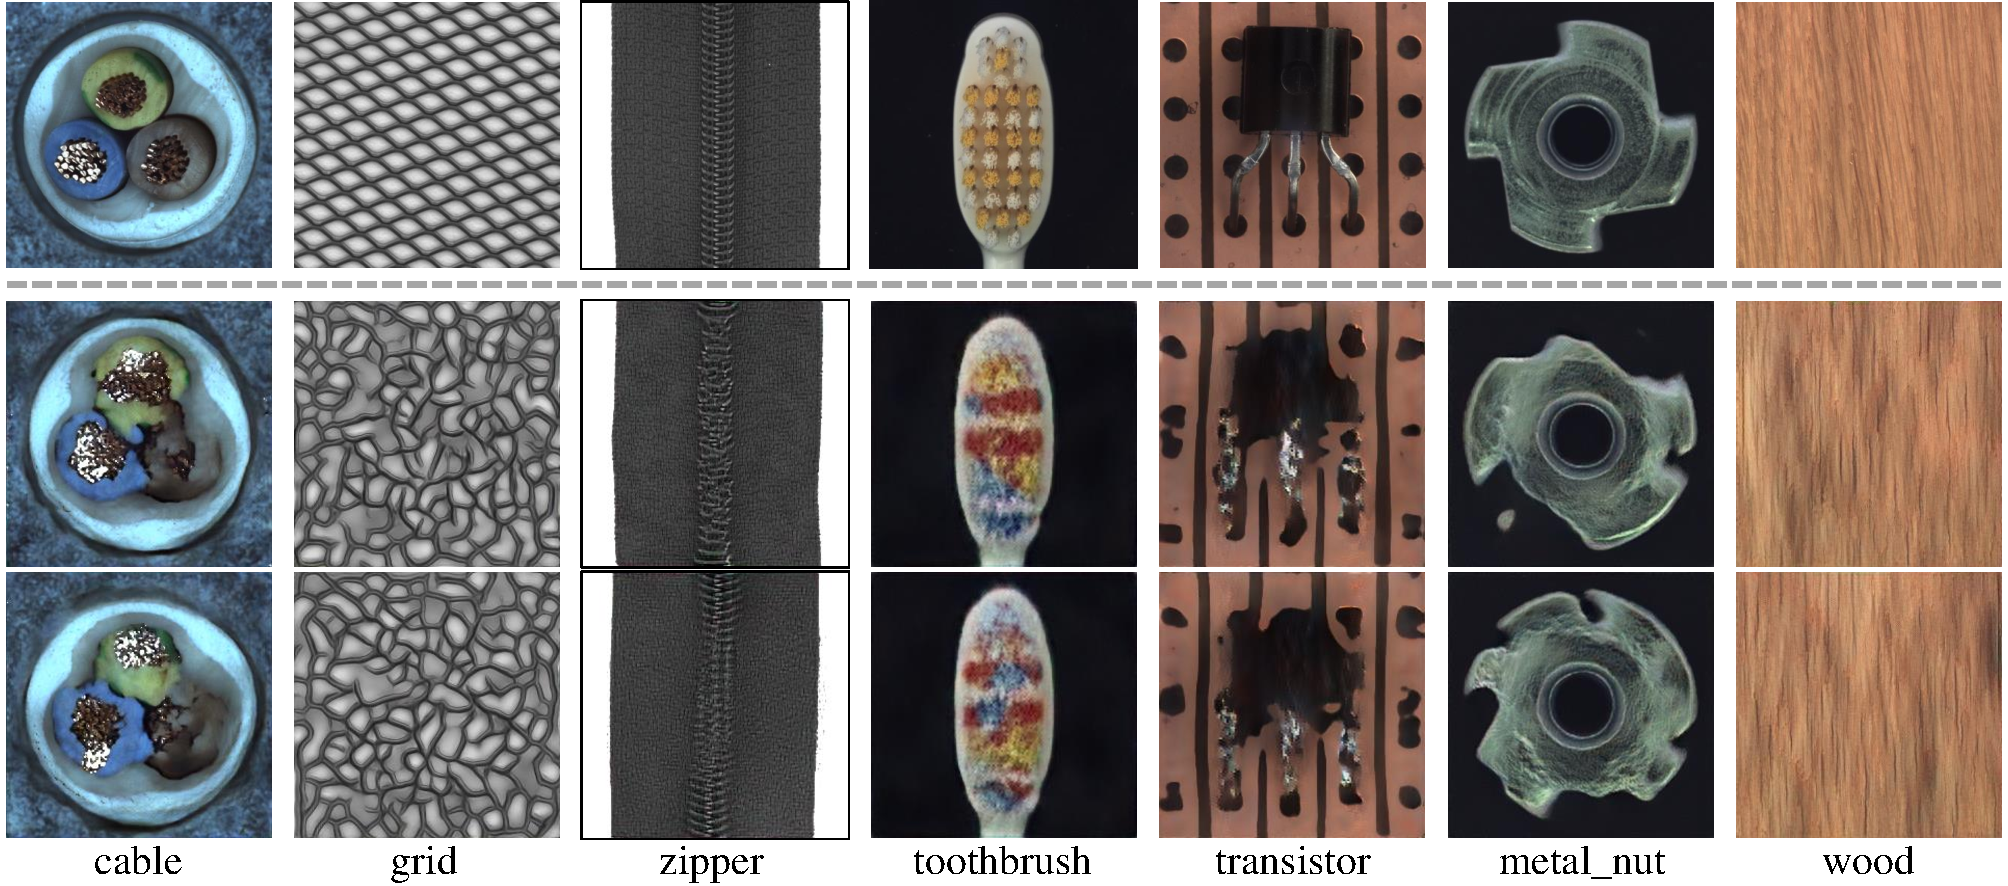
\includegraphics[width=0.7\linewidth]{images/mvtec_generation_results.pdf}
    \caption{Contrastive images generated by level-13 PatchDiff for MVTec AD~\cite{MVTecAD}. } 
    \label{fig: mvtec_generation}
\end{figure*}

\begin{table*}[!h]
    \centering
    % \footnotesize
    % \setlength{\belowcaptionskip}{0.2cm}
    % \setlength{\abovecaptionskip}{0.0cm}
    \renewcommand{\arraystretch}{1.2}
    \resizebox{\textwidth}{!}
    {
\begin{tabular}{cl|c|c|c|c|c|c|c|c}
\toprule
% \multicolumn{2}{c|}{Category} & \makecell[c]{IGD\\\tiny{\citealp{IGD}}} & \makecell[c]{PSVDD\\\tiny{\citealp{PSVDD}}} & \makecell[c]{FCDD\\\tiny{\citealp{FCDD}}} & \makecell[c]{CutPaste\\\tiny{\citealp{CutPaste}}} & \makecell[c]{NSA\\\tiny{\citealp{NSA}}} & \makecell[c]{DRAEM\\\tiny{\citealp{DRAEM}}} & \makecell[c]{DSR\\\tiny{\citealp{DSR}}} & \makecell[c]{GRAD\\\tiny{Ours}} \\ \midrule
\multicolumn{2}{c|}{Category}     & IGD & PSVDD & FCDD & CutPaste &NSA & DRAEM & DSR & GRAD \\ \midrule
\multirow{5}{*}{Texture} 
& carpet & (94.7, 82.8 ) & (92.9, 92.6) & (96.0, - ) & (93.1, 98.3) & (95.5, 95.6) & (95.5,97.0) & (-, \textbf{100.}) & (\textbf{96.5}, 98.2) \\
& grid & (97.7, 97.8 ) & (94.6, 100.) & (91.0, - ) & (\textbf{99.9}, 97.5) & (99.2, 99.9) & (99.7, 99.9) & (-, \textbf{100.}) & (97.2, \textbf{100.}) \\
& leather & (99.5, 95.8) & (90.9, 98.6) & (98.0, - ) & (\textbf{100.}, 99.5) & (99.5, 99.9) & (98.6, \textbf{100.}) & (-, \textbf{100.}) & (98.8, \textbf{100.}) \\
& tile & (78.0, 99.1) & (97.8, 91.4) & (91.0, - ) & (93.4, 90.5) & (\textbf{99.3}, \textbf{100.}) & (99.2, 99.6) & (-, \textbf{100.}) & (95.4, \textbf{100.}) \\
& wood & (89.1, 94.6) & (96.5, 90.8) & (88.0, - ) & (\textbf{98.6}, 95.5) & (90.7, 97.5) & (96.4, \textbf{99.1}) & (-, 96.3) & (87.2, 98.3) \\
\midrule
\multirow{10}{*}{Object} 
& bottle & (92.2, \textbf{100.}) & (98.6, 98.1) & (97.0, - ) & (98.3, 97.6) & (98.3, 97.7) & (\textbf{99.1}, 99.2) & (-, \textbf{100.}) & (96.5, \textbf{100.}) \\
& cable & (84.7, 90.6) & (90.3, 96.8) & (90.0, - ) & (80.6, 90.0) & (96.0, 94.5) & (94.7, 91.8) & (-, 93.8) & (\textbf{98.4}, \textbf{99.3}) \\
& capsule & (\textbf{97.7}, 91.5) & (76.7, 95.8) & (93.0, - ) & (96.2, 97.4) & (97.6, 95.2) & (94.3, \textbf{98.5}) & (-, 98.1) & (97.1, 96.4) \\
& hazelnut & (98.0, 99.7) & (92.0, 97.5) & (95.0, - ) & (97.3, 97.3) & (97.6, 94.7) & (\textbf{99.7}, \textbf{100.}) & (-, 95.6) & (96.6, 98.1) \\
& metal nut & (92.6, 91.3) & (94.0, 98.0) & (94.0, - ) & (99.3, 93.1) & (98.4, 98.7) & (\textbf{99.5}, 98.7) & (-, 98.5) & (93.7, \textbf{100.}) \\
& pill & (97.3, 87.3) & (86.1, 95.1) & (81.0, - ) & (92.4, 95.7) & (\textbf{98.5}, \textbf{99.2}) & (97.6, 98.9) & (-, 97.5) & (98.1, 95.7) \\
& screw & (97.0, 82.5) & (81.3, 95.7) & (86.0, - ) & (86.3, \textbf{96.7}) & (96.5, 90.2) & (97.6, 93.9) & (-, 96.2) & (\textbf{99.2}, 96.0) \\
& toothbrush & (97.7, 99.7) & (\textbf{100.}, 98.1) & (94.0, - ) & (98.3, 98.1) & (94.9, \textbf{100.}) & (98.1, \textbf{100.}) & (-, 99.7) & (98.0, 99.7) \\
& transistor & (84.4, 90.6) & (91.5, 97.0) & (88.0, - ) & (95.5, 93.0) & (88.0, 95.1) & (90.9, 93.1) & (-, 97.8) & (\textbf{97.8}, \textbf{100.}) \\
& zipper & (96.7, 97.0) & (97.9, 95.1) & (92.0, - ) & (\textbf{99.4}, 99.3) & (94.2, 99.8) & (98.9, \textbf{100.}) & (-, \textbf{100.}) & (98.3, 99.7) \\
\midrule
\multicolumn{2}{c|}{Average} & (93.1, 93.4) & (92.5, 93.2 ) & (92.1, 95.7) & (95.2, 96.0) & (96.3, 97.2) & (\textbf{97.3}, 98.0) & (-, 98.2) & (96.8, \textbf{98.7}) \\
\bottomrule
\end{tabular}}
\caption{Anomaly detection performance on MVTec AD dataset~\cite{MVTecAD}. Both pixel-level (left) and image-level (right) AUROC results are shown in each column. The best results are in bold.}
\label{tab: mvtec_main_detail}
\end{table*}

\subsection{Anomaly Detection and Localization}
In the main body, we exclusively present the averaged performance comparison on MVTec AD. In this section, we extend our analysis to provide a detailed result of the anomaly detection and localization performance across each individual sub-dataset within MVTec AD, and display anomaly maps on MVTec AD in Fig.~\ref{fig: main_mvtec_ad_results}. As shown in Table~\ref{tab: mvtec_main_detail}, we compare GRAD to IGD~\cite{IGD}, PSVDD~\cite{PSVDD}, FCDD~\cite{FCDD}, CutPaste~\cite{CutPaste}, NSA~\cite{NSA}, DRAEM~\cite{DRAEM}, and DSR~\cite{DSR}, all of which are independent of pretrained feature extractors. It is easy to find GRAD achieves a strong detection and localization of anomalies.  

\begin{figure*}[!h]
    \centering
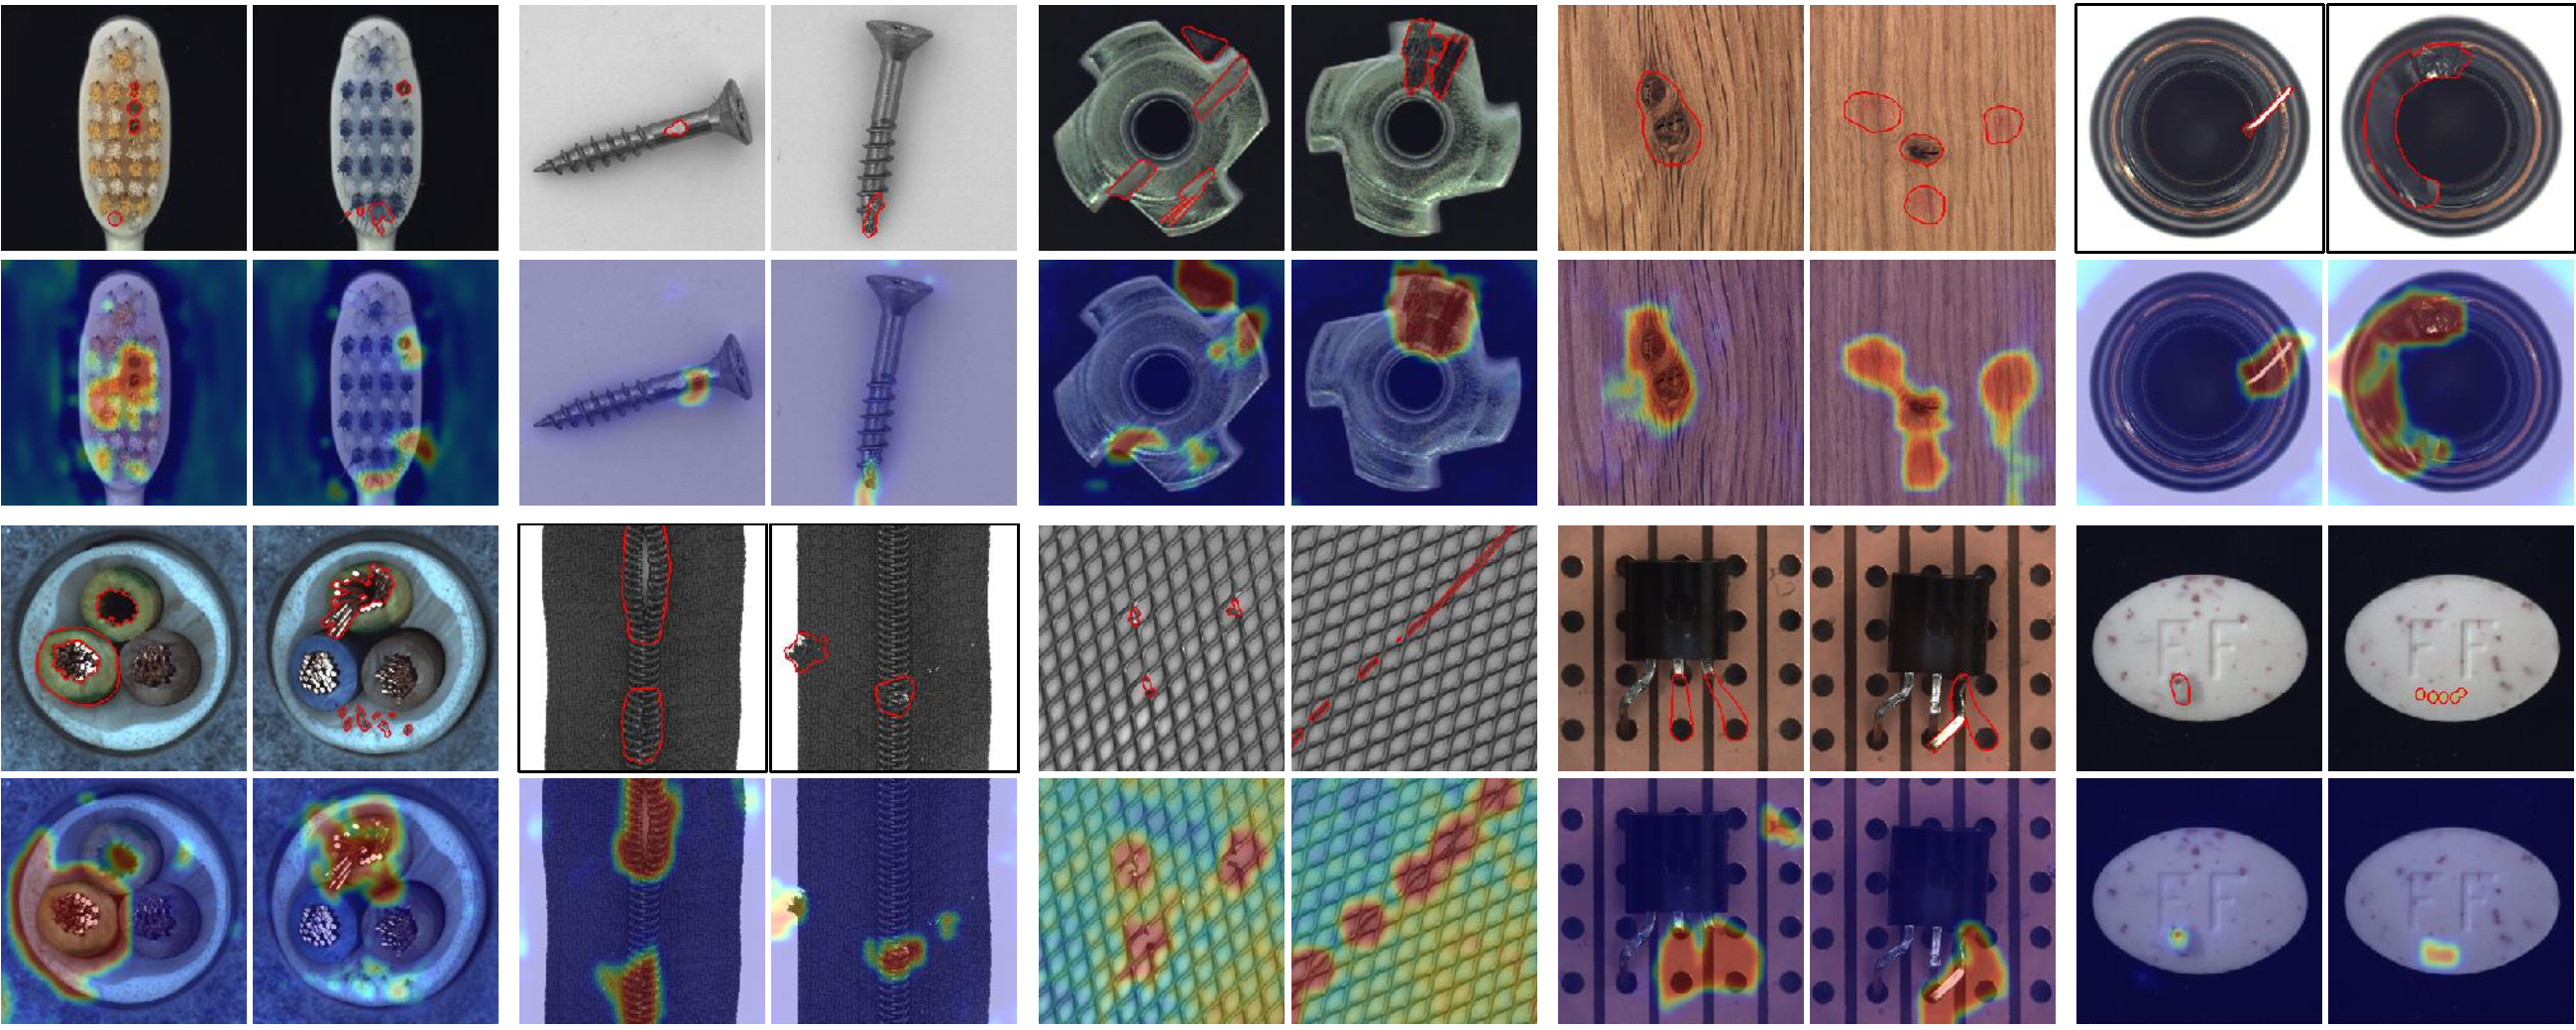
\includegraphics[width=0.9\linewidth]{images/mvtec_results.pdf}
    \caption{Defect localization results of GRAD on MVTec AD~\cite{MVTecAD}. } 
    \label{fig: main_mvtec_ad_results}
    % \vspace{-0.2cm}
\end{figure*}


% In addition, as shown in Table~\ref{tab:ablation_GRad_level}, we conduct an ablations study on selecting levels of patch-level detectors. It is easy to find that when integrating all three different levels of detectors, GRAD can achieve a strong performance for the detection of structural as well as logical anomalies.

% \begin{table}[!htbp]
% \centering
% \footnotesize
% \resizebox{0.3\textwidth}{!}{
% \begin{tabular}{ccc|c}
% \toprule
% \multicolumn{3}{c|}{Level Settings}& Image-level \\
% 136 & 68 & 34  & AUROC\\
% \midrule
% \checkmark &   \ding{55} & \ding{55}   &  85.2   \\
% \ding{55}& \checkmark & \ding{55} & 85.4 \\
% \ding{55}&\ding{55} & \checkmark & 75.1\\
% \checkmark & \checkmark & \ding{55}   &  86.8     \\ %
% \checkmark &   \ding{55} & \checkmark   &  86.4   \\
% \ding{55} & \checkmark & \checkmark  & 86.2 \\
% \checkmark & \checkmark & \checkmark &  \textbf{87.5}  \\
% \bottomrule
% \end{tabular}}
% \caption{Ablation study on detector levels. Detection AUROC results on MVTec LOCO dataset. The best results are in bold.}
% \label{tab:ablation_GRad_level}
% \end{table}



% \bibliography{aaai24}
% \bibliographystyle{aaai24}

% \end{document}




\end{document}